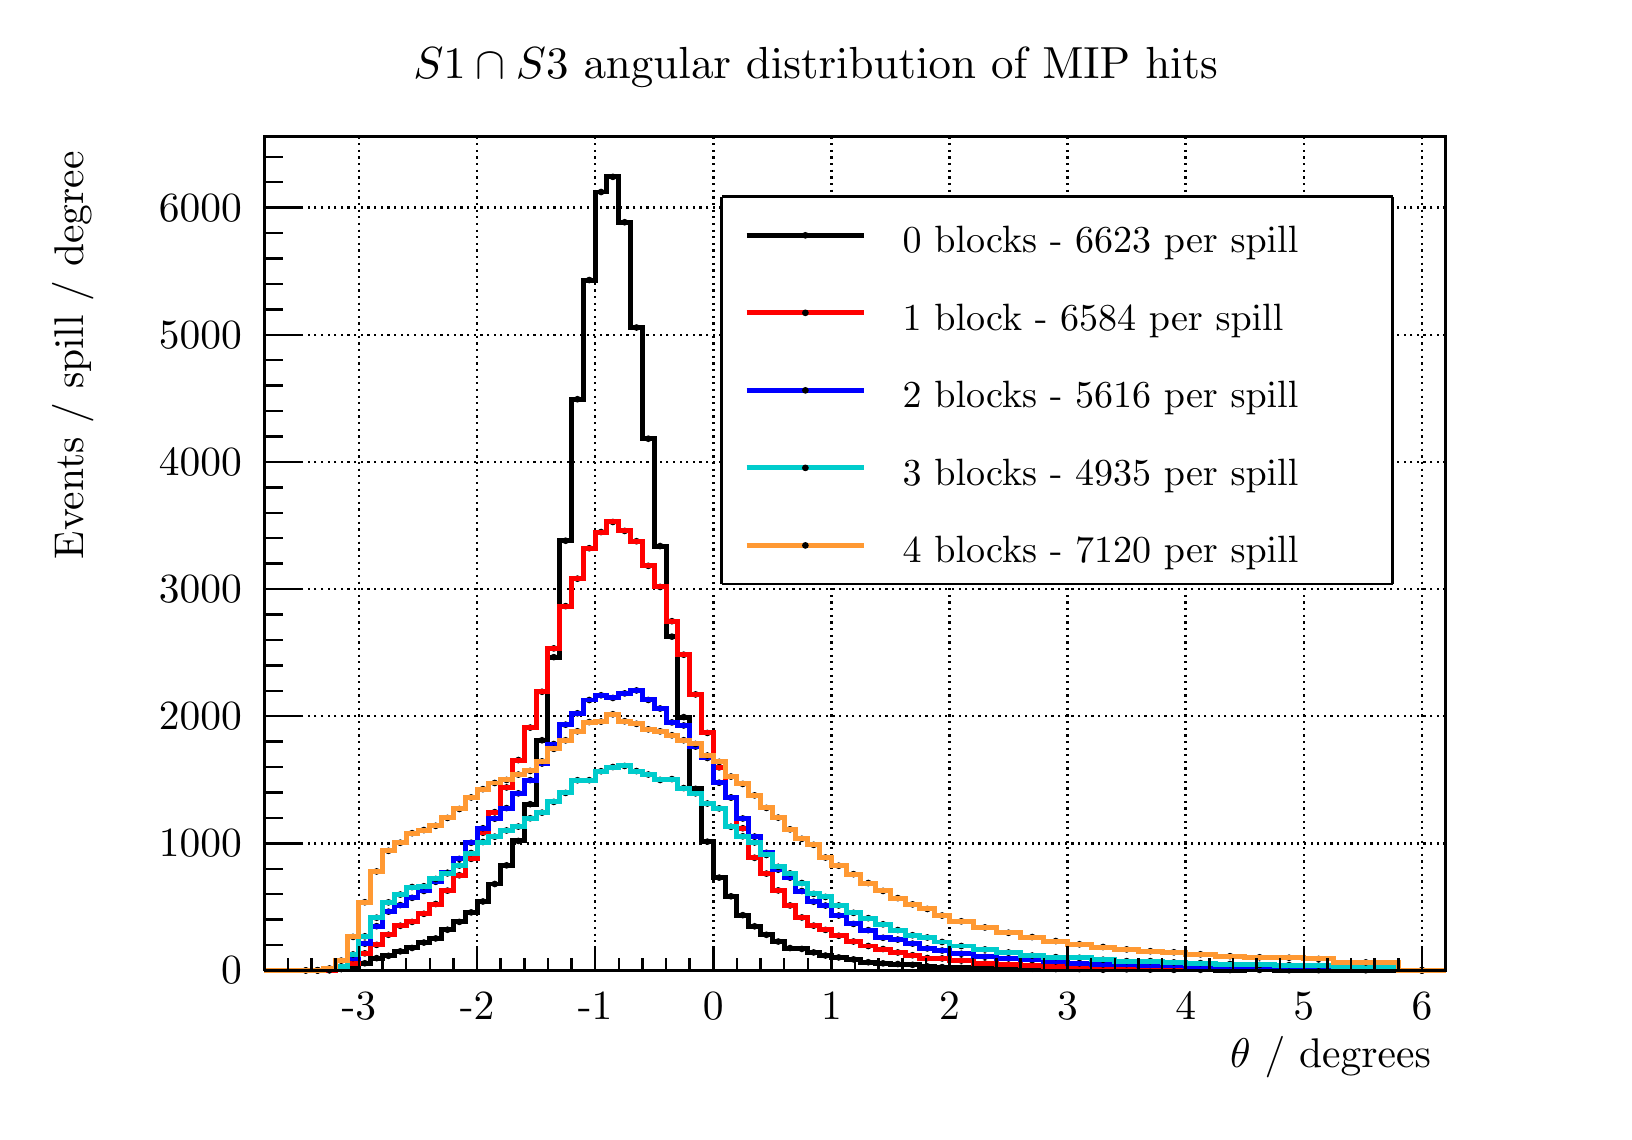
\begin{tikzpicture}
\pgfdeclareplotmark{cross} {
\pgfpathmoveto{\pgfpoint{-0.3\pgfplotmarksize}{\pgfplotmarksize}}
\pgfpathlineto{\pgfpoint{+0.3\pgfplotmarksize}{\pgfplotmarksize}}
\pgfpathlineto{\pgfpoint{+0.3\pgfplotmarksize}{0.3\pgfplotmarksize}}
\pgfpathlineto{\pgfpoint{+1\pgfplotmarksize}{0.3\pgfplotmarksize}}
\pgfpathlineto{\pgfpoint{+1\pgfplotmarksize}{-0.3\pgfplotmarksize}}
\pgfpathlineto{\pgfpoint{+0.3\pgfplotmarksize}{-0.3\pgfplotmarksize}}
\pgfpathlineto{\pgfpoint{+0.3\pgfplotmarksize}{-1.\pgfplotmarksize}}
\pgfpathlineto{\pgfpoint{-0.3\pgfplotmarksize}{-1.\pgfplotmarksize}}
\pgfpathlineto{\pgfpoint{-0.3\pgfplotmarksize}{-0.3\pgfplotmarksize}}
\pgfpathlineto{\pgfpoint{-1.\pgfplotmarksize}{-0.3\pgfplotmarksize}}
\pgfpathlineto{\pgfpoint{-1.\pgfplotmarksize}{0.3\pgfplotmarksize}}
\pgfpathlineto{\pgfpoint{-0.3\pgfplotmarksize}{0.3\pgfplotmarksize}}
\pgfpathclose
\pgfusepathqstroke
}
\pgfdeclareplotmark{cross*} {
\pgfpathmoveto{\pgfpoint{-0.3\pgfplotmarksize}{\pgfplotmarksize}}
\pgfpathlineto{\pgfpoint{+0.3\pgfplotmarksize}{\pgfplotmarksize}}
\pgfpathlineto{\pgfpoint{+0.3\pgfplotmarksize}{0.3\pgfplotmarksize}}
\pgfpathlineto{\pgfpoint{+1\pgfplotmarksize}{0.3\pgfplotmarksize}}
\pgfpathlineto{\pgfpoint{+1\pgfplotmarksize}{-0.3\pgfplotmarksize}}
\pgfpathlineto{\pgfpoint{+0.3\pgfplotmarksize}{-0.3\pgfplotmarksize}}
\pgfpathlineto{\pgfpoint{+0.3\pgfplotmarksize}{-1.\pgfplotmarksize}}
\pgfpathlineto{\pgfpoint{-0.3\pgfplotmarksize}{-1.\pgfplotmarksize}}
\pgfpathlineto{\pgfpoint{-0.3\pgfplotmarksize}{-0.3\pgfplotmarksize}}
\pgfpathlineto{\pgfpoint{-1.\pgfplotmarksize}{-0.3\pgfplotmarksize}}
\pgfpathlineto{\pgfpoint{-1.\pgfplotmarksize}{0.3\pgfplotmarksize}}
\pgfpathlineto{\pgfpoint{-0.3\pgfplotmarksize}{0.3\pgfplotmarksize}}
\pgfpathclose
\pgfusepathqfillstroke
}
\pgfdeclareplotmark{newstar} {
\pgfpathmoveto{\pgfqpoint{0pt}{\pgfplotmarksize}}
\pgfpathlineto{\pgfqpointpolar{44}{0.5\pgfplotmarksize}}
\pgfpathlineto{\pgfqpointpolar{18}{\pgfplotmarksize}}
\pgfpathlineto{\pgfqpointpolar{-20}{0.5\pgfplotmarksize}}
\pgfpathlineto{\pgfqpointpolar{-54}{\pgfplotmarksize}}
\pgfpathlineto{\pgfqpointpolar{-90}{0.5\pgfplotmarksize}}
\pgfpathlineto{\pgfqpointpolar{234}{\pgfplotmarksize}}
\pgfpathlineto{\pgfqpointpolar{198}{0.5\pgfplotmarksize}}
\pgfpathlineto{\pgfqpointpolar{162}{\pgfplotmarksize}}
\pgfpathlineto{\pgfqpointpolar{134}{0.5\pgfplotmarksize}}
\pgfpathclose
\pgfusepathqstroke
}
\pgfdeclareplotmark{newstar*} {
\pgfpathmoveto{\pgfqpoint{0pt}{\pgfplotmarksize}}
\pgfpathlineto{\pgfqpointpolar{44}{0.5\pgfplotmarksize}}
\pgfpathlineto{\pgfqpointpolar{18}{\pgfplotmarksize}}
\pgfpathlineto{\pgfqpointpolar{-20}{0.5\pgfplotmarksize}}
\pgfpathlineto{\pgfqpointpolar{-54}{\pgfplotmarksize}}
\pgfpathlineto{\pgfqpointpolar{-90}{0.5\pgfplotmarksize}}
\pgfpathlineto{\pgfqpointpolar{234}{\pgfplotmarksize}}
\pgfpathlineto{\pgfqpointpolar{198}{0.5\pgfplotmarksize}}
\pgfpathlineto{\pgfqpointpolar{162}{\pgfplotmarksize}}
\pgfpathlineto{\pgfqpointpolar{134}{0.5\pgfplotmarksize}}
\pgfpathclose
\pgfusepathqfillstroke
}
\definecolor{c}{rgb}{1,1,1};
\draw [color=c, fill=c] (0,0) rectangle (20,13.7553);
\draw [color=c, fill=c] (3,1.78819) rectangle (18,12.3797);
\definecolor{c}{rgb}{0,0,0};
\draw [c,line width=0.9] (3,1.78819) -- (3,12.3797) -- (18,12.3797) -- (18,1.78819) -- (3,1.78819);
\definecolor{c}{rgb}{1,1,1};
\draw [color=c, fill=c] (3,1.78819) rectangle (18,12.3797);
\definecolor{c}{rgb}{0,0,0};
\draw [c,line width=0.9] (3,1.78819) -- (3,12.3797) -- (18,12.3797) -- (18,1.78819) -- (3,1.78819);
\draw [c,line width=0.9] (3,1.78819) -- (18,1.78819);
\draw [c,dash pattern=on 0.80pt off 1.60pt ,line width=0.9] (4.2,12.3797) -- (4.2,1.78819);
\draw [c,dash pattern=on 0.80pt off 1.60pt ,line width=0.9] (5.7,12.3797) -- (5.7,1.78819);
\draw [c,dash pattern=on 0.80pt off 1.60pt ,line width=0.9] (7.2,12.3797) -- (7.2,1.78819);
\draw [c,dash pattern=on 0.80pt off 1.60pt ,line width=0.9] (8.7,12.3797) -- (8.7,1.78819);
\draw [c,dash pattern=on 0.80pt off 1.60pt ,line width=0.9] (10.2,12.3797) -- (10.2,1.78819);
\draw [c,dash pattern=on 0.80pt off 1.60pt ,line width=0.9] (11.7,12.3797) -- (11.7,1.78819);
\draw [c,dash pattern=on 0.80pt off 1.60pt ,line width=0.9] (13.2,12.3797) -- (13.2,1.78819);
\draw [c,dash pattern=on 0.80pt off 1.60pt ,line width=0.9] (14.7,12.3797) -- (14.7,1.78819);
\draw [c,dash pattern=on 0.80pt off 1.60pt ,line width=0.9] (16.2,12.3797) -- (16.2,1.78819);
\draw [c,dash pattern=on 0.80pt off 1.60pt ,line width=0.9] (17.7,12.3797) -- (17.7,1.78819);
\draw [c,dash pattern=on 0.80pt off 1.60pt ,line width=0.9] (4.2,12.3797) -- (4.2,1.78819);
\draw [c,dash pattern=on 0.80pt off 1.60pt ,line width=0.9] (17.7,12.3797) -- (17.7,1.78819);
\draw [c,line width=0.9] (3,1.78819) -- (3,12.3797);
\draw [c,dash pattern=on 0.80pt off 1.60pt ,line width=0.9] (18,1.78819) -- (3,1.78819);
\draw [c,dash pattern=on 0.80pt off 1.60pt ,line width=0.9] (18,3.40289) -- (3,3.40289);
\draw [c,dash pattern=on 0.80pt off 1.60pt ,line width=0.9] (18,5.0176) -- (3,5.0176);
\draw [c,dash pattern=on 0.80pt off 1.60pt ,line width=0.9] (18,6.6323) -- (3,6.6323);
\draw [c,dash pattern=on 0.80pt off 1.60pt ,line width=0.9] (18,8.247) -- (3,8.247);
\draw [c,dash pattern=on 0.80pt off 1.60pt ,line width=0.9] (18,9.86171) -- (3,9.86171);
\draw [c,dash pattern=on 0.80pt off 1.60pt ,line width=0.9] (18,11.4764) -- (3,11.4764);
\draw [c,dash pattern=on 0.80pt off 1.60pt ,line width=0.9] (18,11.4764) -- (3,11.4764);
\definecolor{c}{rgb}{0,0,0.6};
\draw [c,line width=0.9] (3,1.78819) -- (3.15,1.78819) -- (3.15,1.78819) -- (3.3,1.78819) -- (3.3,1.78819) -- (3.45,1.78819) -- (3.45,1.78819) -- (3.6,1.78819) -- (3.6,1.78819) -- (3.75,1.78819) -- (3.75,1.78819) -- (3.9,1.78819) -- (3.9,1.78819) --
 (4.05,1.78819) -- (4.05,1.78819) -- (4.2,1.78819) -- (4.2,1.78819) -- (4.35,1.78819) -- (4.35,1.78819) -- (4.5,1.78819) -- (4.5,1.78819) -- (4.65,1.78819) -- (4.65,1.78819) -- (4.8,1.78819) -- (4.8,1.78819) -- (4.95,1.78819) -- (4.95,1.78819) --
 (5.1,1.78819) -- (5.1,1.78819) -- (5.25,1.78819) -- (5.25,1.78819) -- (5.4,1.78819) -- (5.4,1.78819) -- (5.55,1.78819) -- (5.55,1.78819) -- (5.7,1.78819) -- (5.7,1.78819) -- (5.85,1.78819) -- (5.85,1.78819) -- (6,1.78819) -- (6,1.78819) --
 (6.15,1.78819) -- (6.15,1.78819) -- (6.3,1.78819) -- (6.3,1.78819) -- (6.45,1.78819) -- (6.45,1.78819) -- (6.6,1.78819) -- (6.6,1.78819) -- (6.75,1.78819) -- (6.75,1.78819) -- (6.9,1.78819) -- (6.9,1.78819) -- (7.05,1.78819) -- (7.05,1.78819) --
 (7.2,1.78819) -- (7.2,1.78819) -- (7.35,1.78819) -- (7.35,1.78819) -- (7.5,1.78819) -- (7.5,1.78819) -- (7.65,1.78819) -- (7.65,1.78819) -- (7.8,1.78819) -- (7.8,1.78819) -- (7.95,1.78819) -- (7.95,1.78819) -- (8.1,1.78819) -- (8.1,1.78819) --
 (8.25,1.78819) -- (8.25,1.78819) -- (8.4,1.78819) -- (8.4,1.78819) -- (8.55,1.78819) -- (8.55,1.78819) -- (8.7,1.78819) -- (8.7,1.78819) -- (8.85,1.78819) -- (8.85,1.78819) -- (9,1.78819) -- (9,1.78819) -- (9.15,1.78819) -- (9.15,1.78819) --
 (9.3,1.78819) -- (9.3,1.78819) -- (9.45,1.78819) -- (9.45,1.78819) -- (9.6,1.78819) -- (9.6,1.78819) -- (9.75,1.78819) -- (9.75,1.78819) -- (9.9,1.78819) -- (9.9,1.78819) -- (10.05,1.78819) -- (10.05,1.78819) -- (10.2,1.78819) -- (10.2,1.78819) --
 (10.3875,1.78819) -- (10.3875,1.78819) -- (10.575,1.78819) -- (10.575,1.78819) -- (10.7625,1.78819) -- (10.7625,1.78819) -- (10.95,1.78819) -- (10.95,1.78819) -- (11.1375,1.78819) -- (11.1375,1.78819) -- (11.325,1.78819) -- (11.325,1.78819) --
 (11.5125,1.78819) -- (11.5125,1.78819) -- (11.7,1.78819) -- (11.7,1.78819) -- (12,1.78819) -- (12,1.78819) -- (12.3,1.78819) -- (12.3,1.78819) -- (12.6,1.78819) -- (12.6,1.78819) -- (12.9,1.78819) -- (12.9,1.78819) -- (13.2,1.78819) --
 (13.2,1.78819) -- (13.5,1.78819) -- (13.5,1.78819) -- (13.8,1.78819) -- (13.8,1.78819) -- (14.1,1.78819) -- (14.1,1.78819) -- (14.4,1.78819) -- (14.4,1.78819) -- (14.7,1.78819) -- (14.7,1.78819) -- (15.075,1.78819) -- (15.075,1.78819) --
 (15.45,1.78819) -- (15.45,1.78819) -- (15.825,1.78819) -- (15.825,1.78819) -- (16.2,1.78819) -- (16.2,1.78819) -- (16.575,1.78819) -- (16.575,1.78819) -- (17.4,1.78819) -- (17.4,1.78819) -- (18,1.78819);
\definecolor{c}{rgb}{0,0,0};
\draw [c,line width=0.9] (3,1.78819) -- (18,1.78819);
\draw [c,line width=0.9] (4.2,2.09768) -- (4.2,1.78819);
\draw [c,line width=0.9] (4.5,1.94293) -- (4.5,1.78819);
\draw [c,line width=0.9] (4.8,1.94293) -- (4.8,1.78819);
\draw [c,line width=0.9] (5.1,1.94293) -- (5.1,1.78819);
\draw [c,line width=0.9] (5.4,1.94293) -- (5.4,1.78819);
\draw [c,line width=0.9] (5.7,2.09768) -- (5.7,1.78819);
\draw [c,line width=0.9] (6,1.94293) -- (6,1.78819);
\draw [c,line width=0.9] (6.3,1.94293) -- (6.3,1.78819);
\draw [c,line width=0.9] (6.6,1.94293) -- (6.6,1.78819);
\draw [c,line width=0.9] (6.9,1.94293) -- (6.9,1.78819);
\draw [c,line width=0.9] (7.2,2.09768) -- (7.2,1.78819);
\draw [c,line width=0.9] (7.5,1.94293) -- (7.5,1.78819);
\draw [c,line width=0.9] (7.8,1.94293) -- (7.8,1.78819);
\draw [c,line width=0.9] (8.1,1.94293) -- (8.1,1.78819);
\draw [c,line width=0.9] (8.4,1.94293) -- (8.4,1.78819);
\draw [c,line width=0.9] (8.7,2.09768) -- (8.7,1.78819);
\draw [c,line width=0.9] (9,1.94293) -- (9,1.78819);
\draw [c,line width=0.9] (9.3,1.94293) -- (9.3,1.78819);
\draw [c,line width=0.9] (9.6,1.94293) -- (9.6,1.78819);
\draw [c,line width=0.9] (9.9,1.94293) -- (9.9,1.78819);
\draw [c,line width=0.9] (10.2,2.09768) -- (10.2,1.78819);
\draw [c,line width=0.9] (10.5,1.94293) -- (10.5,1.78819);
\draw [c,line width=0.9] (10.8,1.94293) -- (10.8,1.78819);
\draw [c,line width=0.9] (11.1,1.94293) -- (11.1,1.78819);
\draw [c,line width=0.9] (11.4,1.94293) -- (11.4,1.78819);
\draw [c,line width=0.9] (11.7,2.09768) -- (11.7,1.78819);
\draw [c,line width=0.9] (12,1.94293) -- (12,1.78819);
\draw [c,line width=0.9] (12.3,1.94293) -- (12.3,1.78819);
\draw [c,line width=0.9] (12.6,1.94293) -- (12.6,1.78819);
\draw [c,line width=0.9] (12.9,1.94293) -- (12.9,1.78819);
\draw [c,line width=0.9] (13.2,2.09768) -- (13.2,1.78819);
\draw [c,line width=0.9] (13.5,1.94293) -- (13.5,1.78819);
\draw [c,line width=0.9] (13.8,1.94293) -- (13.8,1.78819);
\draw [c,line width=0.9] (14.1,1.94293) -- (14.1,1.78819);
\draw [c,line width=0.9] (14.4,1.94293) -- (14.4,1.78819);
\draw [c,line width=0.9] (14.7,2.09768) -- (14.7,1.78819);
\draw [c,line width=0.9] (15,1.94293) -- (15,1.78819);
\draw [c,line width=0.9] (15.3,1.94293) -- (15.3,1.78819);
\draw [c,line width=0.9] (15.6,1.94293) -- (15.6,1.78819);
\draw [c,line width=0.9] (15.9,1.94293) -- (15.9,1.78819);
\draw [c,line width=0.9] (16.2,2.09768) -- (16.2,1.78819);
\draw [c,line width=0.9] (16.5,1.94293) -- (16.5,1.78819);
\draw [c,line width=0.9] (16.8,1.94293) -- (16.8,1.78819);
\draw [c,line width=0.9] (17.1,1.94293) -- (17.1,1.78819);
\draw [c,line width=0.9] (17.4,1.94293) -- (17.4,1.78819);
\draw [c,line width=0.9] (17.7,2.09768) -- (17.7,1.78819);
\draw [c,line width=0.9] (4.2,2.09768) -- (4.2,1.78819);
\draw [c,line width=0.9] (3.9,1.94293) -- (3.9,1.78819);
\draw [c,line width=0.9] (3.6,1.94293) -- (3.6,1.78819);
\draw [c,line width=0.9] (3.3,1.94293) -- (3.3,1.78819);
\draw [c,line width=0.9] (3,1.94293) -- (3,1.78819);
\draw [c,line width=0.9] (17.7,2.09768) -- (17.7,1.78819);
\draw [c,line width=0.9] (18,1.94293) -- (18,1.78819);
\draw [anchor=base] (4.2,1.1692) node[scale=1.49939, color=c, rotate=0]{-3};
\draw [anchor=base] (5.7,1.1692) node[scale=1.49939, color=c, rotate=0]{-2};
\draw [anchor=base] (7.2,1.1692) node[scale=1.49939, color=c, rotate=0]{-1};
\draw [anchor=base] (8.7,1.1692) node[scale=1.49939, color=c, rotate=0]{0};
\draw [anchor=base] (10.2,1.1692) node[scale=1.49939, color=c, rotate=0]{1};
\draw [anchor=base] (11.7,1.1692) node[scale=1.49939, color=c, rotate=0]{2};
\draw [anchor=base] (13.2,1.1692) node[scale=1.49939, color=c, rotate=0]{3};
\draw [anchor=base] (14.7,1.1692) node[scale=1.49939, color=c, rotate=0]{4};
\draw [anchor=base] (16.2,1.1692) node[scale=1.49939, color=c, rotate=0]{5};
\draw [anchor=base] (17.7,1.1692) node[scale=1.49939, color=c, rotate=0]{6};
\draw [anchor= east] (18,0.687764) node[scale=1.49939, color=c, rotate=0]{$ \theta$ / degrees};
\draw [c,line width=0.9] (3,1.78819) -- (3,12.3797);
\draw [c,line width=0.9] (3.462,1.78819) -- (3,1.78819);
\draw [c,line width=0.9] (3.231,2.11113) -- (3,2.11113);
\draw [c,line width=0.9] (3.231,2.43407) -- (3,2.43407);
\draw [c,line width=0.9] (3.231,2.75701) -- (3,2.75701);
\draw [c,line width=0.9] (3.231,3.07995) -- (3,3.07995);
\draw [c,line width=0.9] (3.462,3.40289) -- (3,3.40289);
\draw [c,line width=0.9] (3.231,3.72583) -- (3,3.72583);
\draw [c,line width=0.9] (3.231,4.04877) -- (3,4.04877);
\draw [c,line width=0.9] (3.231,4.37171) -- (3,4.37171);
\draw [c,line width=0.9] (3.231,4.69465) -- (3,4.69465);
\draw [c,line width=0.9] (3.462,5.0176) -- (3,5.0176);
\draw [c,line width=0.9] (3.231,5.34054) -- (3,5.34054);
\draw [c,line width=0.9] (3.231,5.66348) -- (3,5.66348);
\draw [c,line width=0.9] (3.231,5.98642) -- (3,5.98642);
\draw [c,line width=0.9] (3.231,6.30936) -- (3,6.30936);
\draw [c,line width=0.9] (3.462,6.6323) -- (3,6.6323);
\draw [c,line width=0.9] (3.231,6.95524) -- (3,6.95524);
\draw [c,line width=0.9] (3.231,7.27818) -- (3,7.27818);
\draw [c,line width=0.9] (3.231,7.60112) -- (3,7.60112);
\draw [c,line width=0.9] (3.231,7.92406) -- (3,7.92406);
\draw [c,line width=0.9] (3.462,8.247) -- (3,8.247);
\draw [c,line width=0.9] (3.231,8.56995) -- (3,8.56995);
\draw [c,line width=0.9] (3.231,8.89289) -- (3,8.89289);
\draw [c,line width=0.9] (3.231,9.21583) -- (3,9.21583);
\draw [c,line width=0.9] (3.231,9.53877) -- (3,9.53877);
\draw [c,line width=0.9] (3.462,9.86171) -- (3,9.86171);
\draw [c,line width=0.9] (3.231,10.1847) -- (3,10.1847);
\draw [c,line width=0.9] (3.231,10.5076) -- (3,10.5076);
\draw [c,line width=0.9] (3.231,10.8305) -- (3,10.8305);
\draw [c,line width=0.9] (3.231,11.1535) -- (3,11.1535);
\draw [c,line width=0.9] (3.462,11.4764) -- (3,11.4764);
\draw [c,line width=0.9] (3.462,11.4764) -- (3,11.4764);
\draw [c,line width=0.9] (3.231,11.7994) -- (3,11.7994);
\draw [c,line width=0.9] (3.231,12.1223) -- (3,12.1223);
\draw [anchor= east] (2.9,1.78819) node[scale=1.49939, color=c, rotate=0]{0};
\draw [anchor= east] (2.9,3.40289) node[scale=1.49939, color=c, rotate=0]{1000};
\draw [anchor= east] (2.9,5.0176) node[scale=1.49939, color=c, rotate=0]{2000};
\draw [anchor= east] (2.9,6.6323) node[scale=1.49939, color=c, rotate=0]{3000};
\draw [anchor= east] (2.9,8.247) node[scale=1.49939, color=c, rotate=0]{4000};
\draw [anchor= east] (2.9,9.86171) node[scale=1.49939, color=c, rotate=0]{5000};
\draw [anchor= east] (2.9,11.4764) node[scale=1.49939, color=c, rotate=0]{6000};
\draw [anchor= east] (0.565401,12.3797) node[scale=1.49939, color=c, rotate=90]{ Events / spill / degree};
\draw [c,line width=1.8] (3.825,1.79792) -- (3.825,1.79817);
\draw [c,line width=1.8] (3.825,1.79817) -- (3.825,1.79842);
\foreach \P in {(3.825,1.79817)}{\draw[mark options={color=c,fill=c},mark size=2.402402pt,mark=*,mark size=1pt] plot coordinates {\P};}
\draw [c,line width=1.8] (3.975,1.80842) -- (3.975,1.80877);
\draw [c,line width=1.8] (3.975,1.80877) -- (3.975,1.80913);
\foreach \P in {(3.975,1.80877)}{\draw[mark options={color=c,fill=c},mark size=2.402402pt,mark=*,mark size=1pt] plot coordinates {\P};}
\draw [c,line width=1.8] (4.125,1.84002) -- (4.125,1.84059);
\draw [c,line width=1.8] (4.125,1.84059) -- (4.125,1.84117);
\foreach \P in {(4.125,1.84059)}{\draw[mark options={color=c,fill=c},mark size=2.402402pt,mark=*,mark size=1pt] plot coordinates {\P};}
\draw [c,line width=1.8] (4.275,1.87977) -- (4.275,1.88052);
\draw [c,line width=1.8] (4.275,1.88052) -- (4.275,1.88128);
\foreach \P in {(4.275,1.88052)}{\draw[mark options={color=c,fill=c},mark size=2.402402pt,mark=*,mark size=1pt] plot coordinates {\P};}
\draw [c,line width=1.8] (4.425,1.94442) -- (4.425,1.94541);
\draw [c,line width=1.8] (4.425,1.94541) -- (4.425,1.9464);
\foreach \P in {(4.425,1.94541)}{\draw[mark options={color=c,fill=c},mark size=2.402402pt,mark=*,mark size=1pt] plot coordinates {\P};}
\draw [c,line width=1.8] (4.575,1.97366) -- (4.575,1.97473);
\draw [c,line width=1.8] (4.575,1.97473) -- (4.575,1.97581);
\foreach \P in {(4.575,1.97473)}{\draw[mark options={color=c,fill=c},mark size=2.402402pt,mark=*,mark size=1pt] plot coordinates {\P};}
\draw [c,line width=1.8] (4.725,2.03028) -- (4.725,2.03151);
\draw [c,line width=1.8] (4.725,2.03151) -- (4.725,2.03274);
\foreach \P in {(4.725,2.03151)}{\draw[mark options={color=c,fill=c},mark size=2.402402pt,mark=*,mark size=1pt] plot coordinates {\P};}
\draw [c,line width=1.8] (4.875,2.07322) -- (4.875,2.07456);
\draw [c,line width=1.8] (4.875,2.07456) -- (4.875,2.0759);
\foreach \P in {(4.875,2.07456)}{\draw[mark options={color=c,fill=c},mark size=2.402402pt,mark=*,mark size=1pt] plot coordinates {\P};}
\draw [c,line width=1.8] (5.025,2.1417) -- (5.025,2.14319);
\draw [c,line width=1.8] (5.025,2.14319) -- (5.025,2.14468);
\foreach \P in {(5.025,2.14319)}{\draw[mark options={color=c,fill=c},mark size=2.402402pt,mark=*,mark size=1pt] plot coordinates {\P};}
\draw [c,line width=1.8] (5.175,2.194) -- (5.175,2.1956);
\draw [c,line width=1.8] (5.175,2.1956) -- (5.175,2.19719);
\foreach \P in {(5.175,2.1956)}{\draw[mark options={color=c,fill=c},mark size=2.402402pt,mark=*,mark size=1pt] plot coordinates {\P};}
\draw [c,line width=1.8] (5.325,2.30423) -- (5.325,2.30603);
\draw [c,line width=1.8] (5.325,2.30603) -- (5.325,2.30783);
\foreach \P in {(5.325,2.30603)}{\draw[mark options={color=c,fill=c},mark size=2.402402pt,mark=*,mark size=1pt] plot coordinates {\P};}
\draw [c,line width=1.8] (5.475,2.40389) -- (5.475,2.40586);
\draw [c,line width=1.8] (5.475,2.40586) -- (5.475,2.40782);
\foreach \P in {(5.475,2.40586)}{\draw[mark options={color=c,fill=c},mark size=2.402402pt,mark=*,mark size=1pt] plot coordinates {\P};}
\draw [c,line width=1.8] (5.625,2.52413) -- (5.625,2.52627);
\draw [c,line width=1.8] (5.625,2.52627) -- (5.625,2.52842);
\foreach \P in {(5.625,2.52627)}{\draw[mark options={color=c,fill=c},mark size=2.402402pt,mark=*,mark size=1pt] plot coordinates {\P};}
\draw [c,line width=1.8] (5.775,2.66244) -- (5.775,2.66478);
\draw [c,line width=1.8] (5.775,2.66478) -- (5.775,2.66712);
\foreach \P in {(5.775,2.66478)}{\draw[mark options={color=c,fill=c},mark size=2.402402pt,mark=*,mark size=1pt] plot coordinates {\P};}
\draw [c,line width=1.8] (5.925,2.88427) -- (5.925,2.88689);
\draw [c,line width=1.8] (5.925,2.88689) -- (5.925,2.88951);
\foreach \P in {(5.925,2.88689)}{\draw[mark options={color=c,fill=c},mark size=2.402402pt,mark=*,mark size=1pt] plot coordinates {\P};}
\draw [c,line width=1.8] (6.075,3.12109) -- (6.075,3.12398);
\draw [c,line width=1.8] (6.075,3.12398) -- (6.075,3.12686);
\foreach \P in {(6.075,3.12398)}{\draw[mark options={color=c,fill=c},mark size=2.402402pt,mark=*,mark size=1pt] plot coordinates {\P};}
\draw [c,line width=1.8] (6.225,3.43086) -- (6.225,3.43406);
\draw [c,line width=1.8] (6.225,3.43406) -- (6.225,3.43727);
\foreach \P in {(6.225,3.43406)}{\draw[mark options={color=c,fill=c},mark size=2.402402pt,mark=*,mark size=1pt] plot coordinates {\P};}
\draw [c,line width=1.8] (6.375,3.89712) -- (6.375,3.90075);
\draw [c,line width=1.8] (6.375,3.90075) -- (6.375,3.90438);
\foreach \P in {(6.375,3.90075)}{\draw[mark options={color=c,fill=c},mark size=2.402402pt,mark=*,mark size=1pt] plot coordinates {\P};}
\draw [c,line width=1.8] (6.525,4.70818) -- (6.525,4.71245);
\draw [c,line width=1.8] (6.525,4.71245) -- (6.525,4.71672);
\foreach \P in {(6.525,4.71245)}{\draw[mark options={color=c,fill=c},mark size=2.402402pt,mark=*,mark size=1pt] plot coordinates {\P};}
\draw [c,line width=1.8] (6.675,5.76313) -- (6.675,5.76811);
\draw [c,line width=1.8] (6.675,5.76811) -- (6.675,5.77309);
\foreach \P in {(6.675,5.76811)}{\draw[mark options={color=c,fill=c},mark size=2.402402pt,mark=*,mark size=1pt] plot coordinates {\P};}
\draw [c,line width=1.8] (6.825,7.24032) -- (6.825,7.24615);
\draw [c,line width=1.8] (6.825,7.24615) -- (6.825,7.25199);
\foreach \P in {(6.825,7.24615)}{\draw[mark options={color=c,fill=c},mark size=2.402402pt,mark=*,mark size=1pt] plot coordinates {\P};}
\draw [c,line width=1.8] (6.975,9.03691) -- (6.975,9.04364);
\draw [c,line width=1.8] (6.975,9.04364) -- (6.975,9.05037);
\foreach \P in {(6.975,9.04364)}{\draw[mark options={color=c,fill=c},mark size=2.402402pt,mark=*,mark size=1pt] plot coordinates {\P};}
\draw [c,line width=1.8] (7.125,10.5498) -- (7.125,10.5572);
\draw [c,line width=1.8] (7.125,10.5572) -- (7.125,10.5646);
\foreach \P in {(7.125,10.5572)}{\draw[mark options={color=c,fill=c},mark size=2.402402pt,mark=*,mark size=1pt] plot coordinates {\P};}
\draw [c,line width=1.8] (7.275,11.6674) -- (7.275,11.6753);
\draw [c,line width=1.8] (7.275,11.6753) -- (7.275,11.6831);
\foreach \P in {(7.275,11.6753)}{\draw[mark options={color=c,fill=c},mark size=2.402402pt,mark=*,mark size=1pt] plot coordinates {\P};}
\draw [c,line width=1.8] (7.425,11.8595) -- (7.425,11.8675);
\draw [c,line width=1.8] (7.425,11.8675) -- (7.425,11.8754);
\foreach \P in {(7.425,11.8675)}{\draw[mark options={color=c,fill=c},mark size=2.402402pt,mark=*,mark size=1pt] plot coordinates {\P};}
\draw [c,line width=1.8] (7.575,11.2833) -- (7.575,11.291);
\draw [c,line width=1.8] (7.575,11.291) -- (7.575,11.2987);
\foreach \P in {(7.575,11.291)}{\draw[mark options={color=c,fill=c},mark size=2.402402pt,mark=*,mark size=1pt] plot coordinates {\P};}
\draw [c,line width=1.8] (7.725,9.94679) -- (7.725,9.95392);
\draw [c,line width=1.8] (7.725,9.95392) -- (7.725,9.96106);
\foreach \P in {(7.725,9.95392)}{\draw[mark options={color=c,fill=c},mark size=2.402402pt,mark=*,mark size=1pt] plot coordinates {\P};}
\draw [c,line width=1.8] (7.875,8.53552) -- (7.875,8.54201);
\draw [c,line width=1.8] (7.875,8.54201) -- (7.875,8.54851);
\foreach \P in {(7.875,8.54201)}{\draw[mark options={color=c,fill=c},mark size=2.402402pt,mark=*,mark size=1pt] plot coordinates {\P};}
\draw [c,line width=1.8] (8.025,7.17297) -- (8.025,7.17877);
\draw [c,line width=1.8] (8.025,7.17877) -- (8.025,7.18457);
\foreach \P in {(8.025,7.17877)}{\draw[mark options={color=c,fill=c},mark size=2.402402pt,mark=*,mark size=1pt] plot coordinates {\P};}
\draw [c,line width=1.8] (8.175,6.02314) -- (8.175,6.02828);
\draw [c,line width=1.8] (8.175,6.02828) -- (8.175,6.03342);
\foreach \P in {(8.175,6.02828)}{\draw[mark options={color=c,fill=c},mark size=2.402402pt,mark=*,mark size=1pt] plot coordinates {\P};}
\draw [c,line width=1.8] (8.325,5.00183) -- (8.325,5.00631);
\draw [c,line width=1.8] (8.325,5.00631) -- (8.325,5.0108);
\foreach \P in {(8.325,5.00631)}{\draw[mark options={color=c,fill=c},mark size=2.402402pt,mark=*,mark size=1pt] plot coordinates {\P};}
\draw [c,line width=1.8] (8.475,4.09161) -- (8.475,4.09541);
\draw [c,line width=1.8] (8.475,4.09541) -- (8.475,4.0992);
\foreach \P in {(8.475,4.09541)}{\draw[mark options={color=c,fill=c},mark size=2.402402pt,mark=*,mark size=1pt] plot coordinates {\P};}
\draw [c,line width=1.8] (8.625,3.42151) -- (8.625,3.4247);
\draw [c,line width=1.8] (8.625,3.4247) -- (8.625,3.4279);
\foreach \P in {(8.625,3.4247)}{\draw[mark options={color=c,fill=c},mark size=2.402402pt,mark=*,mark size=1pt] plot coordinates {\P};}
\draw [c,line width=1.8] (8.775,2.96529) -- (8.775,2.968);
\draw [c,line width=1.8] (8.775,2.968) -- (8.775,2.97071);
\foreach \P in {(8.775,2.968)}{\draw[mark options={color=c,fill=c},mark size=2.402402pt,mark=*,mark size=1pt] plot coordinates {\P};}
\draw [c,line width=1.8] (8.925,2.72849) -- (8.925,2.73091);
\draw [c,line width=1.8] (8.925,2.73091) -- (8.925,2.73334);
\foreach \P in {(8.925,2.73091)}{\draw[mark options={color=c,fill=c},mark size=2.402402pt,mark=*,mark size=1pt] plot coordinates {\P};}
\draw [c,line width=1.8] (9.075,2.48924) -- (9.075,2.49133);
\draw [c,line width=1.8] (9.075,2.49133) -- (9.075,2.49343);
\foreach \P in {(9.075,2.49133)}{\draw[mark options={color=c,fill=c},mark size=2.402402pt,mark=*,mark size=1pt] plot coordinates {\P};}
\draw [c,line width=1.8] (9.225,2.34783) -- (9.225,2.3497);
\draw [c,line width=1.8] (9.225,2.3497) -- (9.225,2.35158);
\foreach \P in {(9.225,2.3497)}{\draw[mark options={color=c,fill=c},mark size=2.402402pt,mark=*,mark size=1pt] plot coordinates {\P};}
\draw [c,line width=1.8] (9.375,2.24009) -- (9.375,2.24177);
\draw [c,line width=1.8] (9.375,2.24177) -- (9.375,2.24345);
\foreach \P in {(9.375,2.24177)}{\draw[mark options={color=c,fill=c},mark size=2.402402pt,mark=*,mark size=1pt] plot coordinates {\P};}
\draw [c,line width=1.8] (9.525,2.15478) -- (9.525,2.15629);
\draw [c,line width=1.8] (9.525,2.15629) -- (9.525,2.15781);
\foreach \P in {(9.525,2.15629)}{\draw[mark options={color=c,fill=c},mark size=2.402402pt,mark=*,mark size=1pt] plot coordinates {\P};}
\draw [c,line width=1.8] (9.675,2.07198) -- (9.675,2.07331);
\draw [c,line width=1.8] (9.675,2.07331) -- (9.675,2.07465);
\foreach \P in {(9.675,2.07331)}{\draw[mark options={color=c,fill=c},mark size=2.402402pt,mark=*,mark size=1pt] plot coordinates {\P};}
\draw [c,line width=1.8] (9.825,2.0614) -- (9.825,2.06271);
\draw [c,line width=1.8] (9.825,2.06271) -- (9.825,2.06401);
\foreach \P in {(9.825,2.06271)}{\draw[mark options={color=c,fill=c},mark size=2.402402pt,mark=*,mark size=1pt] plot coordinates {\P};}
\draw [c,line width=1.8] (9.975,2.01659) -- (9.975,2.01778);
\draw [c,line width=1.8] (9.975,2.01778) -- (9.975,2.01898);
\foreach \P in {(9.975,2.01778)}{\draw[mark options={color=c,fill=c},mark size=2.402402pt,mark=*,mark size=1pt] plot coordinates {\P};}
\draw [c,line width=1.8] (10.125,1.97739) -- (10.125,1.97848);
\draw [c,line width=1.8] (10.125,1.97848) -- (10.125,1.97957);
\foreach \P in {(10.125,1.97848)}{\draw[mark options={color=c,fill=c},mark size=2.402402pt,mark=*,mark size=1pt] plot coordinates {\P};}
\draw [c,line width=1.8] (10.2937,1.95326) -- (10.2937,1.9544);
\draw [c,line width=1.8] (10.2937,1.9544) -- (10.2937,1.95553);
\foreach \P in {(10.2937,1.9544)}{\draw[mark options={color=c,fill=c},mark size=2.402402pt,mark=*,mark size=1pt] plot coordinates {\P};}
\draw [c,line width=1.8] (10.4812,1.92839) -- (10.4812,1.92944);
\draw [c,line width=1.8] (10.4812,1.92944) -- (10.4812,1.93049);
\foreach \P in {(10.4812,1.92944)}{\draw[mark options={color=c,fill=c},mark size=2.402402pt,mark=*,mark size=1pt] plot coordinates {\P};}
\draw [c,line width=1.8] (10.6687,1.8926) -- (10.6687,1.8935);
\draw [c,line width=1.8] (10.6687,1.8935) -- (10.6687,1.89441);
\foreach \P in {(10.6687,1.8935)}{\draw[mark options={color=c,fill=c},mark size=2.402402pt,mark=*,mark size=1pt] plot coordinates {\P};}
\draw [c,line width=1.8] (10.8562,1.87819) -- (10.8562,1.87903);
\draw [c,line width=1.8] (10.8562,1.87903) -- (10.8562,1.87987);
\foreach \P in {(10.8562,1.87903)}{\draw[mark options={color=c,fill=c},mark size=2.402402pt,mark=*,mark size=1pt] plot coordinates {\P};}
\draw [c,line width=1.8] (11.0437,1.86974) -- (11.0437,1.87054);
\draw [c,line width=1.8] (11.0437,1.87054) -- (11.0437,1.87134);
\foreach \P in {(11.0437,1.87054)}{\draw[mark options={color=c,fill=c},mark size=2.402402pt,mark=*,mark size=1pt] plot coordinates {\P};}
\draw [c,line width=1.8] (11.2312,1.85981) -- (11.2312,1.86056);
\draw [c,line width=1.8] (11.2312,1.86056) -- (11.2312,1.86131);
\foreach \P in {(11.2312,1.86056)}{\draw[mark options={color=c,fill=c},mark size=2.402402pt,mark=*,mark size=1pt] plot coordinates {\P};}
\draw [c,line width=1.8] (11.4187,1.84045) -- (11.4187,1.84109);
\draw [c,line width=1.8] (11.4187,1.84109) -- (11.4187,1.84174);
\foreach \P in {(11.4187,1.84109)}{\draw[mark options={color=c,fill=c},mark size=2.402402pt,mark=*,mark size=1pt] plot coordinates {\P};}
\draw [c,line width=1.8] (11.6062,1.83053) -- (11.6062,1.83111);
\draw [c,line width=1.8] (11.6062,1.83111) -- (11.6062,1.83169);
\foreach \P in {(11.6062,1.83111)}{\draw[mark options={color=c,fill=c},mark size=2.402402pt,mark=*,mark size=1pt] plot coordinates {\P};}
\draw [c,line width=1.8] (11.85,1.82123) -- (11.85,1.82188);
\draw [c,line width=1.8] (11.85,1.82188) -- (11.85,1.82253);
\foreach \P in {(11.85,1.82188)}{\draw[mark options={color=c,fill=c},mark size=2.402402pt,mark=*,mark size=1pt] plot coordinates {\P};}
\draw [c,line width=1.8] (12.15,1.81907) -- (12.15,1.81969);
\draw [c,line width=1.8] (12.15,1.81969) -- (12.15,1.82032);
\foreach \P in {(12.15,1.81969)}{\draw[mark options={color=c,fill=c},mark size=2.402402pt,mark=*,mark size=1pt] plot coordinates {\P};}
\draw [c,line width=1.8] (12.45,1.81444) -- (12.45,1.81501);
\draw [c,line width=1.8] (12.45,1.81501) -- (12.45,1.81559);
\foreach \P in {(12.45,1.81501)}{\draw[mark options={color=c,fill=c},mark size=2.402402pt,mark=*,mark size=1pt] plot coordinates {\P};}
\draw [c,line width=1.8] (12.75,1.81104) -- (12.75,1.81158);
\draw [c,line width=1.8] (12.75,1.81158) -- (12.75,1.81212);
\foreach \P in {(12.75,1.81158)}{\draw[mark options={color=c,fill=c},mark size=2.402402pt,mark=*,mark size=1pt] plot coordinates {\P};}
\draw [c,line width=1.8] (13.05,1.80642) -- (13.05,1.8069);
\draw [c,line width=1.8] (13.05,1.8069) -- (13.05,1.80739);
\foreach \P in {(13.05,1.8069)}{\draw[mark options={color=c,fill=c},mark size=2.402402pt,mark=*,mark size=1pt] plot coordinates {\P};}
\draw [c,line width=1.8] (13.35,1.8055) -- (13.35,1.80597);
\draw [c,line width=1.8] (13.35,1.80597) -- (13.35,1.80644);
\foreach \P in {(13.35,1.80597)}{\draw[mark options={color=c,fill=c},mark size=2.402402pt,mark=*,mark size=1pt] plot coordinates {\P};}
\draw [c,line width=1.8] (13.65,1.79751) -- (13.65,1.79786);
\draw [c,line width=1.8] (13.65,1.79786) -- (13.65,1.7982);
\foreach \P in {(13.65,1.79786)}{\draw[mark options={color=c,fill=c},mark size=2.402402pt,mark=*,mark size=1pt] plot coordinates {\P};}
\draw [c,line width=1.8] (13.95,1.80334) -- (13.95,1.80378);
\draw [c,line width=1.8] (13.95,1.80378) -- (13.95,1.80422);
\foreach \P in {(13.95,1.80378)}{\draw[mark options={color=c,fill=c},mark size=2.402402pt,mark=*,mark size=1pt] plot coordinates {\P};}
\draw [c,line width=1.8] (14.25,1.79935) -- (14.25,1.79973);
\draw [c,line width=1.8] (14.25,1.79973) -- (14.25,1.80011);
\foreach \P in {(14.25,1.79973)}{\draw[mark options={color=c,fill=c},mark size=2.402402pt,mark=*,mark size=1pt] plot coordinates {\P};}
\draw [c,line width=1.8] (14.55,1.79628) -- (14.55,1.79661);
\draw [c,line width=1.8] (14.55,1.79661) -- (14.55,1.79693);
\foreach \P in {(14.55,1.79661)}{\draw[mark options={color=c,fill=c},mark size=2.402402pt,mark=*,mark size=1pt] plot coordinates {\P};}
\draw [c,line width=1.8] (14.8875,1.79753) -- (14.8875,1.79792);
\draw [c,line width=1.8] (14.8875,1.79792) -- (14.8875,1.79831);
\foreach \P in {(14.8875,1.79792)}{\draw[mark options={color=c,fill=c},mark size=2.402402pt,mark=*,mark size=1pt] plot coordinates {\P};}
\draw [c,line width=1.8] (15.2625,1.79387) -- (15.2625,1.79418);
\draw [c,line width=1.8] (15.2625,1.79418) -- (15.2625,1.79448);
\foreach \P in {(15.2625,1.79418)}{\draw[mark options={color=c,fill=c},mark size=2.402402pt,mark=*,mark size=1pt] plot coordinates {\P};}
\draw [c,line width=1.8] (15.6375,1.79582) -- (15.6375,1.79617);
\draw [c,line width=1.8] (15.6375,1.79617) -- (15.6375,1.79652);
\foreach \P in {(15.6375,1.79617)}{\draw[mark options={color=c,fill=c},mark size=2.402402pt,mark=*,mark size=1pt] plot coordinates {\P};}
\draw [c,line width=1.8] (16.0125,1.7912) -- (16.0125,1.79143);
\draw [c,line width=1.8] (16.0125,1.79143) -- (16.0125,1.79165);
\foreach \P in {(16.0125,1.79143)}{\draw[mark options={color=c,fill=c},mark size=2.402402pt,mark=*,mark size=1pt] plot coordinates {\P};}
\draw [c,line width=1.8] (16.3875,1.79241) -- (16.3875,1.79268);
\draw [c,line width=1.8] (16.3875,1.79268) -- (16.3875,1.79294);
\foreach \P in {(16.3875,1.79268)}{\draw[mark options={color=c,fill=c},mark size=2.402402pt,mark=*,mark size=1pt] plot coordinates {\P};}
\draw [c,line width=1.8] (16.9875,1.79135) -- (16.9875,1.7917);
\draw [c,line width=1.8] (16.9875,1.7917) -- (16.9875,1.79205);
\foreach \P in {(16.9875,1.7917)}{\draw[mark options={color=c,fill=c},mark size=2.402402pt,mark=*,mark size=1pt] plot coordinates {\P};}
\draw [c,line width=1.8] (17.7,1.78831) -- (17.7,1.78844);
\draw [c,line width=1.8] (17.7,1.78844) -- (17.7,1.78856);
\foreach \P in {(17.7,1.78844)}{\draw[mark options={color=c,fill=c},mark size=2.402402pt,mark=*,mark size=1pt] plot coordinates {\P};}
\draw [c,line width=1.8] (3,1.78819) -- (3.15,1.78819) -- (3.15,1.78819) -- (3.3,1.78819) -- (3.3,1.78819) -- (3.45,1.78819) -- (3.45,1.78819) -- (3.6,1.78819) -- (3.6,1.78819) -- (3.75,1.78819) -- (3.75,1.79817) -- (3.9,1.79817) -- (3.9,1.80877) --
 (4.05,1.80877) -- (4.05,1.84059) -- (4.2,1.84059) -- (4.2,1.88052) -- (4.35,1.88052) -- (4.35,1.94541) -- (4.5,1.94541) -- (4.5,1.97473) -- (4.65,1.97473) -- (4.65,2.03151) -- (4.8,2.03151) -- (4.8,2.07456) -- (4.95,2.07456) -- (4.95,2.14319) --
 (5.1,2.14319) -- (5.1,2.1956) -- (5.25,2.1956) -- (5.25,2.30603) -- (5.4,2.30603) -- (5.4,2.40586) -- (5.55,2.40586) -- (5.55,2.52627) -- (5.7,2.52627) -- (5.7,2.66478) -- (5.85,2.66478) -- (5.85,2.88689) -- (6,2.88689) -- (6,3.12398) --
 (6.15,3.12398) -- (6.15,3.43406) -- (6.3,3.43406) -- (6.3,3.90075) -- (6.45,3.90075) -- (6.45,4.71245) -- (6.6,4.71245) -- (6.6,5.76811) -- (6.75,5.76811) -- (6.75,7.24615) -- (6.9,7.24615) -- (6.9,9.04364) -- (7.05,9.04364) -- (7.05,10.5572) --
 (7.2,10.5572) -- (7.2,11.6753) -- (7.35,11.6753) -- (7.35,11.8675) -- (7.5,11.8675) -- (7.5,11.291) -- (7.65,11.291) -- (7.65,9.95392) -- (7.8,9.95392) -- (7.8,8.54201) -- (7.95,8.54201) -- (7.95,7.17877) -- (8.1,7.17877) -- (8.1,6.02828) --
 (8.25,6.02828) -- (8.25,5.00631) -- (8.4,5.00631) -- (8.4,4.09541) -- (8.55,4.09541) -- (8.55,3.4247) -- (8.7,3.4247) -- (8.7,2.968) -- (8.85,2.968) -- (8.85,2.73091) -- (9,2.73091) -- (9,2.49133) -- (9.15,2.49133) -- (9.15,2.3497) -- (9.3,2.3497)
 -- (9.3,2.24177) -- (9.45,2.24177) -- (9.45,2.15629) -- (9.6,2.15629) -- (9.6,2.07331) -- (9.75,2.07331) -- (9.75,2.06271) -- (9.9,2.06271) -- (9.9,2.01778) -- (10.05,2.01778) -- (10.05,1.97848) -- (10.2,1.97848) -- (10.2,1.9544) -- (10.3875,1.9544)
 -- (10.3875,1.92944) -- (10.575,1.92944) -- (10.575,1.8935) -- (10.7625,1.8935) -- (10.7625,1.87903) -- (10.95,1.87903) -- (10.95,1.87054) -- (11.1375,1.87054) -- (11.1375,1.86056) -- (11.325,1.86056) -- (11.325,1.84109) -- (11.5125,1.84109) --
 (11.5125,1.83111) -- (11.7,1.83111) -- (11.7,1.82188) -- (12,1.82188) -- (12,1.81969) -- (12.3,1.81969) -- (12.3,1.81501) -- (12.6,1.81501) -- (12.6,1.81158) -- (12.9,1.81158) -- (12.9,1.8069) -- (13.2,1.8069) -- (13.2,1.80597) -- (13.5,1.80597) --
 (13.5,1.79786) -- (13.8,1.79786) -- (13.8,1.80378) -- (14.1,1.80378) -- (14.1,1.79973) -- (14.4,1.79973) -- (14.4,1.79661) -- (14.7,1.79661) -- (14.7,1.79792) -- (15.075,1.79792) -- (15.075,1.79418) -- (15.45,1.79418) -- (15.45,1.79617) --
 (15.825,1.79617) -- (15.825,1.79143) -- (16.2,1.79143) -- (16.2,1.79268) -- (16.575,1.79268) -- (16.575,1.7917) -- (17.4,1.7917) -- (17.4,1.78819) -- (18,1.78819);
\definecolor{c}{rgb}{1,0,0};
\draw [c,line width=1.8] (3.675,1.78897) -- (3.675,1.78903);
\draw [c,line width=1.8] (3.675,1.78903) -- (3.675,1.78909);
\definecolor{c}{rgb}{0,0,0};
\foreach \P in {(3.675,1.78903)}{\draw[mark options={color=c,fill=c},mark size=2.402402pt,mark=*,mark size=1pt] plot coordinates {\P};}
\definecolor{c}{rgb}{1,0,0};
\draw [c,line width=1.8] (3.825,1.79029) -- (3.825,1.79039);
\draw [c,line width=1.8] (3.825,1.79039) -- (3.825,1.79049);
\definecolor{c}{rgb}{0,0,0};
\foreach \P in {(3.825,1.79039)}{\draw[mark options={color=c,fill=c},mark size=2.402402pt,mark=*,mark size=1pt] plot coordinates {\P};}
\definecolor{c}{rgb}{1,0,0};
\draw [c,line width=1.8] (3.975,1.80786) -- (3.975,1.80816);
\draw [c,line width=1.8] (3.975,1.80816) -- (3.975,1.80845);
\definecolor{c}{rgb}{0,0,0};
\foreach \P in {(3.975,1.80816)}{\draw[mark options={color=c,fill=c},mark size=2.402402pt,mark=*,mark size=1pt] plot coordinates {\P};}
\definecolor{c}{rgb}{1,0,0};
\draw [c,line width=1.8] (4.125,1.87332) -- (4.125,1.87395);
\draw [c,line width=1.8] (4.125,1.87395) -- (4.125,1.87457);
\definecolor{c}{rgb}{0,0,0};
\foreach \P in {(4.125,1.87395)}{\draw[mark options={color=c,fill=c},mark size=2.402402pt,mark=*,mark size=1pt] plot coordinates {\P};}
\definecolor{c}{rgb}{1,0,0};
\draw [c,line width=1.8] (4.275,2.00505) -- (4.275,2.00604);
\draw [c,line width=1.8] (4.275,2.00604) -- (4.275,2.00703);
\definecolor{c}{rgb}{0,0,0};
\foreach \P in {(4.275,2.00604)}{\draw[mark options={color=c,fill=c},mark size=2.402402pt,mark=*,mark size=1pt] plot coordinates {\P};}
\definecolor{c}{rgb}{1,0,0};
\draw [c,line width=1.8] (4.425,2.11269) -- (4.425,2.1139);
\draw [c,line width=1.8] (4.425,2.1139) -- (4.425,2.11511);
\definecolor{c}{rgb}{0,0,0};
\foreach \P in {(4.425,2.1139)}{\draw[mark options={color=c,fill=c},mark size=2.402402pt,mark=*,mark size=1pt] plot coordinates {\P};}
\definecolor{c}{rgb}{1,0,0};
\draw [c,line width=1.8] (4.575,2.24108) -- (4.575,2.24251);
\draw [c,line width=1.8] (4.575,2.24251) -- (4.575,2.24394);
\definecolor{c}{rgb}{0,0,0};
\foreach \P in {(4.575,2.24251)}{\draw[mark options={color=c,fill=c},mark size=2.402402pt,mark=*,mark size=1pt] plot coordinates {\P};}
\definecolor{c}{rgb}{1,0,0};
\draw [c,line width=1.8] (4.725,2.35512) -- (4.725,2.35672);
\draw [c,line width=1.8] (4.725,2.35672) -- (4.725,2.35832);
\definecolor{c}{rgb}{0,0,0};
\foreach \P in {(4.725,2.35672)}{\draw[mark options={color=c,fill=c},mark size=2.402402pt,mark=*,mark size=1pt] plot coordinates {\P};}
\definecolor{c}{rgb}{1,0,0};
\draw [c,line width=1.8] (4.875,2.404) -- (4.875,2.40566);
\draw [c,line width=1.8] (4.875,2.40566) -- (4.875,2.40731);
\definecolor{c}{rgb}{0,0,0};
\foreach \P in {(4.875,2.40566)}{\draw[mark options={color=c,fill=c},mark size=2.402402pt,mark=*,mark size=1pt] plot coordinates {\P};}
\definecolor{c}{rgb}{1,0,0};
\draw [c,line width=1.8] (5.025,2.50637) -- (5.025,2.50817);
\draw [c,line width=1.8] (5.025,2.50817) -- (5.025,2.50997);
\definecolor{c}{rgb}{0,0,0};
\foreach \P in {(5.025,2.50817)}{\draw[mark options={color=c,fill=c},mark size=2.402402pt,mark=*,mark size=1pt] plot coordinates {\P};}
\definecolor{c}{rgb}{1,0,0};
\draw [c,line width=1.8] (5.175,2.63078) -- (5.175,2.63273);
\draw [c,line width=1.8] (5.175,2.63273) -- (5.175,2.63468);
\definecolor{c}{rgb}{0,0,0};
\foreach \P in {(5.175,2.63273)}{\draw[mark options={color=c,fill=c},mark size=2.402402pt,mark=*,mark size=1pt] plot coordinates {\P};}
\definecolor{c}{rgb}{1,0,0};
\draw [c,line width=1.8] (5.325,2.80071) -- (5.325,2.80285);
\draw [c,line width=1.8] (5.325,2.80285) -- (5.325,2.80498);
\definecolor{c}{rgb}{0,0,0};
\foreach \P in {(5.325,2.80285)}{\draw[mark options={color=c,fill=c},mark size=2.402402pt,mark=*,mark size=1pt] plot coordinates {\P};}
\definecolor{c}{rgb}{1,0,0};
\draw [c,line width=1.8] (5.475,2.99512) -- (5.475,2.99745);
\draw [c,line width=1.8] (5.475,2.99745) -- (5.475,2.99979);
\definecolor{c}{rgb}{0,0,0};
\foreach \P in {(5.475,2.99745)}{\draw[mark options={color=c,fill=c},mark size=2.402402pt,mark=*,mark size=1pt] plot coordinates {\P};}
\definecolor{c}{rgb}{1,0,0};
\draw [c,line width=1.8] (5.625,3.20393) -- (5.625,3.20645);
\draw [c,line width=1.8] (5.625,3.20645) -- (5.625,3.20898);
\definecolor{c}{rgb}{0,0,0};
\foreach \P in {(5.625,3.20645)}{\draw[mark options={color=c,fill=c},mark size=2.402402pt,mark=*,mark size=1pt] plot coordinates {\P};}
\definecolor{c}{rgb}{1,0,0};
\draw [c,line width=1.8] (5.775,3.53507) -- (5.775,3.53787);
\draw [c,line width=1.8] (5.775,3.53787) -- (5.775,3.54067);
\definecolor{c}{rgb}{0,0,0};
\foreach \P in {(5.775,3.53787)}{\draw[mark options={color=c,fill=c},mark size=2.402402pt,mark=*,mark size=1pt] plot coordinates {\P};}
\definecolor{c}{rgb}{1,0,0};
\draw [c,line width=1.8] (5.925,3.79653) -- (5.925,3.79953);
\draw [c,line width=1.8] (5.925,3.79953) -- (5.925,3.80254);
\definecolor{c}{rgb}{0,0,0};
\foreach \P in {(5.925,3.79953)}{\draw[mark options={color=c,fill=c},mark size=2.402402pt,mark=*,mark size=1pt] plot coordinates {\P};}
\definecolor{c}{rgb}{1,0,0};
\draw [c,line width=1.8] (6.075,4.11003) -- (6.075,4.11326);
\draw [c,line width=1.8] (6.075,4.11326) -- (6.075,4.11648);
\definecolor{c}{rgb}{0,0,0};
\foreach \P in {(6.075,4.11326)}{\draw[mark options={color=c,fill=c},mark size=2.402402pt,mark=*,mark size=1pt] plot coordinates {\P};}
\definecolor{c}{rgb}{1,0,0};
\draw [c,line width=1.8] (6.225,4.45761) -- (6.225,4.46107);
\draw [c,line width=1.8] (6.225,4.46107) -- (6.225,4.46453);
\definecolor{c}{rgb}{0,0,0};
\foreach \P in {(6.225,4.46107)}{\draw[mark options={color=c,fill=c},mark size=2.402402pt,mark=*,mark size=1pt] plot coordinates {\P};}
\definecolor{c}{rgb}{1,0,0};
\draw [c,line width=1.8] (6.375,4.86968) -- (6.375,4.8734);
\draw [c,line width=1.8] (6.375,4.8734) -- (6.375,4.87712);
\definecolor{c}{rgb}{0,0,0};
\foreach \P in {(6.375,4.8734)}{\draw[mark options={color=c,fill=c},mark size=2.402402pt,mark=*,mark size=1pt] plot coordinates {\P};}
\definecolor{c}{rgb}{1,0,0};
\draw [c,line width=1.8] (6.525,5.32422) -- (6.525,5.32821);
\draw [c,line width=1.8] (6.525,5.32821) -- (6.525,5.33219);
\definecolor{c}{rgb}{0,0,0};
\foreach \P in {(6.525,5.32821)}{\draw[mark options={color=c,fill=c},mark size=2.402402pt,mark=*,mark size=1pt] plot coordinates {\P};}
\definecolor{c}{rgb}{1,0,0};
\draw [c,line width=1.8] (6.675,5.87498) -- (6.675,5.87926);
\draw [c,line width=1.8] (6.675,5.87926) -- (6.675,5.88354);
\definecolor{c}{rgb}{0,0,0};
\foreach \P in {(6.675,5.87926)}{\draw[mark options={color=c,fill=c},mark size=2.402402pt,mark=*,mark size=1pt] plot coordinates {\P};}
\definecolor{c}{rgb}{1,0,0};
\draw [c,line width=1.8] (6.825,6.41124) -- (6.825,6.4158);
\draw [c,line width=1.8] (6.825,6.4158) -- (6.825,6.42036);
\definecolor{c}{rgb}{0,0,0};
\foreach \P in {(6.825,6.4158)}{\draw[mark options={color=c,fill=c},mark size=2.402402pt,mark=*,mark size=1pt] plot coordinates {\P};}
\definecolor{c}{rgb}{1,0,0};
\draw [c,line width=1.8] (6.975,6.75974) -- (6.975,6.76446);
\draw [c,line width=1.8] (6.975,6.76446) -- (6.975,6.76918);
\definecolor{c}{rgb}{0,0,0};
\foreach \P in {(6.975,6.76446)}{\draw[mark options={color=c,fill=c},mark size=2.402402pt,mark=*,mark size=1pt] plot coordinates {\P};}
\definecolor{c}{rgb}{1,0,0};
\draw [c,line width=1.8] (7.125,7.14636) -- (7.125,7.15125);
\draw [c,line width=1.8] (7.125,7.15125) -- (7.125,7.15615);
\definecolor{c}{rgb}{0,0,0};
\foreach \P in {(7.125,7.15125)}{\draw[mark options={color=c,fill=c},mark size=2.402402pt,mark=*,mark size=1pt] plot coordinates {\P};}
\definecolor{c}{rgb}{1,0,0};
\draw [c,line width=1.8] (7.275,7.35192) -- (7.275,7.35692);
\draw [c,line width=1.8] (7.275,7.35692) -- (7.275,7.36191);
\definecolor{c}{rgb}{0,0,0};
\foreach \P in {(7.275,7.35692)}{\draw[mark options={color=c,fill=c},mark size=2.402402pt,mark=*,mark size=1pt] plot coordinates {\P};}
\definecolor{c}{rgb}{1,0,0};
\draw [c,line width=1.8] (7.425,7.47956) -- (7.425,7.48462);
\draw [c,line width=1.8] (7.425,7.48462) -- (7.425,7.48967);
\definecolor{c}{rgb}{0,0,0};
\foreach \P in {(7.425,7.48462)}{\draw[mark options={color=c,fill=c},mark size=2.402402pt,mark=*,mark size=1pt] plot coordinates {\P};}
\definecolor{c}{rgb}{1,0,0};
\draw [c,line width=1.8] (7.575,7.36587) -- (7.575,7.37088);
\draw [c,line width=1.8] (7.575,7.37088) -- (7.575,7.37588);
\definecolor{c}{rgb}{0,0,0};
\foreach \P in {(7.575,7.37088)}{\draw[mark options={color=c,fill=c},mark size=2.402402pt,mark=*,mark size=1pt] plot coordinates {\P};}
\definecolor{c}{rgb}{1,0,0};
\draw [c,line width=1.8] (7.725,7.23527) -- (7.725,7.24021);
\draw [c,line width=1.8] (7.725,7.24021) -- (7.725,7.24516);
\definecolor{c}{rgb}{0,0,0};
\foreach \P in {(7.725,7.24021)}{\draw[mark options={color=c,fill=c},mark size=2.402402pt,mark=*,mark size=1pt] plot coordinates {\P};}
\definecolor{c}{rgb}{1,0,0};
\draw [c,line width=1.8] (7.875,6.92256) -- (7.875,6.92735);
\draw [c,line width=1.8] (7.875,6.92735) -- (7.875,6.93215);
\definecolor{c}{rgb}{0,0,0};
\foreach \P in {(7.875,6.92735)}{\draw[mark options={color=c,fill=c},mark size=2.402402pt,mark=*,mark size=1pt] plot coordinates {\P};}
\definecolor{c}{rgb}{1,0,0};
\draw [c,line width=1.8] (8.025,6.65478) -- (8.025,6.65946);
\draw [c,line width=1.8] (8.025,6.65946) -- (8.025,6.66413);
\definecolor{c}{rgb}{0,0,0};
\foreach \P in {(8.025,6.65946)}{\draw[mark options={color=c,fill=c},mark size=2.402402pt,mark=*,mark size=1pt] plot coordinates {\P};}
\definecolor{c}{rgb}{1,0,0};
\draw [c,line width=1.8] (8.175,6.22002) -- (8.175,6.22447);
\draw [c,line width=1.8] (8.175,6.22447) -- (8.175,6.22893);
\definecolor{c}{rgb}{0,0,0};
\foreach \P in {(8.175,6.22447)}{\draw[mark options={color=c,fill=c},mark size=2.402402pt,mark=*,mark size=1pt] plot coordinates {\P};}
\definecolor{c}{rgb}{1,0,0};
\draw [c,line width=1.8] (8.325,5.7944) -- (8.325,5.79864);
\draw [c,line width=1.8] (8.325,5.79864) -- (8.325,5.80288);
\definecolor{c}{rgb}{0,0,0};
\foreach \P in {(8.325,5.79864)}{\draw[mark options={color=c,fill=c},mark size=2.402402pt,mark=*,mark size=1pt] plot coordinates {\P};}
\definecolor{c}{rgb}{1,0,0};
\draw [c,line width=1.8] (8.475,5.29068) -- (8.475,5.29464);
\draw [c,line width=1.8] (8.475,5.29464) -- (8.475,5.2986);
\definecolor{c}{rgb}{0,0,0};
\foreach \P in {(8.475,5.29464)}{\draw[mark options={color=c,fill=c},mark size=2.402402pt,mark=*,mark size=1pt] plot coordinates {\P};}
\definecolor{c}{rgb}{1,0,0};
\draw [c,line width=1.8] (8.625,4.80213) -- (8.625,4.80581);
\draw [c,line width=1.8] (8.625,4.80581) -- (8.625,4.80949);
\definecolor{c}{rgb}{0,0,0};
\foreach \P in {(8.625,4.80581)}{\draw[mark options={color=c,fill=c},mark size=2.402402pt,mark=*,mark size=1pt] plot coordinates {\P};}
\definecolor{c}{rgb}{1,0,0};
\draw [c,line width=1.8] (8.775,4.36519) -- (8.775,4.36859);
\draw [c,line width=1.8] (8.775,4.36859) -- (8.775,4.372);
\definecolor{c}{rgb}{0,0,0};
\foreach \P in {(8.775,4.36859)}{\draw[mark options={color=c,fill=c},mark size=2.402402pt,mark=*,mark size=1pt] plot coordinates {\P};}
\definecolor{c}{rgb}{1,0,0};
\draw [c,line width=1.8] (8.925,3.98117) -- (8.925,3.98431);
\draw [c,line width=1.8] (8.925,3.98431) -- (8.925,3.98746);
\definecolor{c}{rgb}{0,0,0};
\foreach \P in {(8.925,3.98431)}{\draw[mark options={color=c,fill=c},mark size=2.402402pt,mark=*,mark size=1pt] plot coordinates {\P};}
\definecolor{c}{rgb}{1,0,0};
\draw [c,line width=1.8] (9.075,3.59139) -- (9.075,3.59423);
\draw [c,line width=1.8] (9.075,3.59423) -- (9.075,3.59707);
\definecolor{c}{rgb}{0,0,0};
\foreach \P in {(9.075,3.59423)}{\draw[mark options={color=c,fill=c},mark size=2.402402pt,mark=*,mark size=1pt] plot coordinates {\P};}
\definecolor{c}{rgb}{1,0,0};
\draw [c,line width=1.8] (9.225,3.21721) -- (9.225,3.21974);
\draw [c,line width=1.8] (9.225,3.21974) -- (9.225,3.22228);
\definecolor{c}{rgb}{0,0,0};
\foreach \P in {(9.225,3.21974)}{\draw[mark options={color=c,fill=c},mark size=2.402402pt,mark=*,mark size=1pt] plot coordinates {\P};}
\definecolor{c}{rgb}{1,0,0};
\draw [c,line width=1.8] (9.375,3.01659) -- (9.375,3.01895);
\draw [c,line width=1.8] (9.375,3.01895) -- (9.375,3.0213);
\definecolor{c}{rgb}{0,0,0};
\foreach \P in {(9.375,3.01895)}{\draw[mark options={color=c,fill=c},mark size=2.402402pt,mark=*,mark size=1pt] plot coordinates {\P};}
\definecolor{c}{rgb}{1,0,0};
\draw [c,line width=1.8] (9.525,2.80343) -- (9.525,2.80557);
\draw [c,line width=1.8] (9.525,2.80557) -- (9.525,2.8077);
\definecolor{c}{rgb}{0,0,0};
\foreach \P in {(9.525,2.80557)}{\draw[mark options={color=c,fill=c},mark size=2.402402pt,mark=*,mark size=1pt] plot coordinates {\P};}
\definecolor{c}{rgb}{1,0,0};
\draw [c,line width=1.8] (9.675,2.61257) -- (9.675,2.6145);
\draw [c,line width=1.8] (9.675,2.6145) -- (9.675,2.61643);
\definecolor{c}{rgb}{0,0,0};
\foreach \P in {(9.675,2.6145)}{\draw[mark options={color=c,fill=c},mark size=2.402402pt,mark=*,mark size=1pt] plot coordinates {\P};}
\definecolor{c}{rgb}{1,0,0};
\draw [c,line width=1.8] (9.825,2.45999) -- (9.825,2.46172);
\draw [c,line width=1.8] (9.825,2.46172) -- (9.825,2.46345);
\definecolor{c}{rgb}{0,0,0};
\foreach \P in {(9.825,2.46172)}{\draw[mark options={color=c,fill=c},mark size=2.402402pt,mark=*,mark size=1pt] plot coordinates {\P};}
\definecolor{c}{rgb}{1,0,0};
\draw [c,line width=1.8] (9.975,2.35654) -- (9.975,2.35814);
\draw [c,line width=1.8] (9.975,2.35814) -- (9.975,2.35974);
\definecolor{c}{rgb}{0,0,0};
\foreach \P in {(9.975,2.35814)}{\draw[mark options={color=c,fill=c},mark size=2.402402pt,mark=*,mark size=1pt] plot coordinates {\P};}
\definecolor{c}{rgb}{1,0,0};
\draw [c,line width=1.8] (10.125,2.30277) -- (10.125,2.3043);
\draw [c,line width=1.8] (10.125,2.3043) -- (10.125,2.30582);
\definecolor{c}{rgb}{0,0,0};
\foreach \P in {(10.125,2.3043)}{\draw[mark options={color=c,fill=c},mark size=2.402402pt,mark=*,mark size=1pt] plot coordinates {\P};}
\definecolor{c}{rgb}{1,0,0};
\draw [c,line width=1.8] (10.2937,2.22793) -- (10.2937,2.2295);
\draw [c,line width=1.8] (10.2937,2.2295) -- (10.2937,2.23107);
\definecolor{c}{rgb}{0,0,0};
\foreach \P in {(10.2937,2.2295)}{\draw[mark options={color=c,fill=c},mark size=2.402402pt,mark=*,mark size=1pt] plot coordinates {\P};}
\definecolor{c}{rgb}{1,0,0};
\draw [c,line width=1.8] (10.4812,2.15492) -- (10.4812,2.15635);
\draw [c,line width=1.8] (10.4812,2.15635) -- (10.4812,2.15779);
\definecolor{c}{rgb}{0,0,0};
\foreach \P in {(10.4812,2.15635)}{\draw[mark options={color=c,fill=c},mark size=2.402402pt,mark=*,mark size=1pt] plot coordinates {\P};}
\definecolor{c}{rgb}{1,0,0};
\draw [c,line width=1.8] (10.6687,2.09822) -- (10.6687,2.09954);
\draw [c,line width=1.8] (10.6687,2.09954) -- (10.6687,2.10086);
\definecolor{c}{rgb}{0,0,0};
\foreach \P in {(10.6687,2.09954)}{\draw[mark options={color=c,fill=c},mark size=2.402402pt,mark=*,mark size=1pt] plot coordinates {\P};}
\definecolor{c}{rgb}{1,0,0};
\draw [c,line width=1.8] (10.8562,2.05965) -- (10.8562,2.06089);
\draw [c,line width=1.8] (10.8562,2.06089) -- (10.8562,2.06213);
\definecolor{c}{rgb}{0,0,0};
\foreach \P in {(10.8562,2.06089)}{\draw[mark options={color=c,fill=c},mark size=2.402402pt,mark=*,mark size=1pt] plot coordinates {\P};}
\definecolor{c}{rgb}{1,0,0};
\draw [c,line width=1.8] (11.0437,2.01634) -- (11.0437,2.01748);
\draw [c,line width=1.8] (11.0437,2.01748) -- (11.0437,2.01861);
\definecolor{c}{rgb}{0,0,0};
\foreach \P in {(11.0437,2.01748)}{\draw[mark options={color=c,fill=c},mark size=2.402402pt,mark=*,mark size=1pt] plot coordinates {\P};}
\definecolor{c}{rgb}{1,0,0};
\draw [c,line width=1.8] (11.2312,1.98118) -- (11.2312,1.98223);
\draw [c,line width=1.8] (11.2312,1.98223) -- (11.2312,1.98328);
\definecolor{c}{rgb}{0,0,0};
\foreach \P in {(11.2312,1.98223)}{\draw[mark options={color=c,fill=c},mark size=2.402402pt,mark=*,mark size=1pt] plot coordinates {\P};}
\definecolor{c}{rgb}{1,0,0};
\draw [c,line width=1.8] (11.4187,1.94575) -- (11.4187,1.94669);
\draw [c,line width=1.8] (11.4187,1.94669) -- (11.4187,1.94763);
\definecolor{c}{rgb}{0,0,0};
\foreach \P in {(11.4187,1.94669)}{\draw[mark options={color=c,fill=c},mark size=2.402402pt,mark=*,mark size=1pt] plot coordinates {\P};}
\definecolor{c}{rgb}{1,0,0};
\draw [c,line width=1.8] (11.6062,1.94093) -- (11.6062,1.94186);
\draw [c,line width=1.8] (11.6062,1.94186) -- (11.6062,1.94279);
\definecolor{c}{rgb}{0,0,0};
\foreach \P in {(11.6062,1.94186)}{\draw[mark options={color=c,fill=c},mark size=2.402402pt,mark=*,mark size=1pt] plot coordinates {\P};}
\definecolor{c}{rgb}{1,0,0};
\draw [c,line width=1.8] (11.85,1.91401) -- (11.85,1.91508);
\draw [c,line width=1.8] (11.85,1.91508) -- (11.85,1.91614);
\definecolor{c}{rgb}{0,0,0};
\foreach \P in {(11.85,1.91508)}{\draw[mark options={color=c,fill=c},mark size=2.402402pt,mark=*,mark size=1pt] plot coordinates {\P};}
\definecolor{c}{rgb}{1,0,0};
\draw [c,line width=1.8] (12.15,1.87655) -- (12.15,1.87745);
\draw [c,line width=1.8] (12.15,1.87745) -- (12.15,1.87834);
\definecolor{c}{rgb}{0,0,0};
\foreach \P in {(12.15,1.87745)}{\draw[mark options={color=c,fill=c},mark size=2.402402pt,mark=*,mark size=1pt] plot coordinates {\P};}
\definecolor{c}{rgb}{1,0,0};
\draw [c,line width=1.8] (12.45,1.85906) -- (12.45,1.85987);
\draw [c,line width=1.8] (12.45,1.85987) -- (12.45,1.86067);
\definecolor{c}{rgb}{0,0,0};
\foreach \P in {(12.45,1.85987)}{\draw[mark options={color=c,fill=c},mark size=2.402402pt,mark=*,mark size=1pt] plot coordinates {\P};}
\definecolor{c}{rgb}{1,0,0};
\draw [c,line width=1.8] (12.75,1.85267) -- (12.75,1.85343);
\draw [c,line width=1.8] (12.75,1.85343) -- (12.75,1.8542);
\definecolor{c}{rgb}{0,0,0};
\foreach \P in {(12.75,1.85343)}{\draw[mark options={color=c,fill=c},mark size=2.402402pt,mark=*,mark size=1pt] plot coordinates {\P};}
\definecolor{c}{rgb}{1,0,0};
\draw [c,line width=1.8] (13.05,1.84307) -- (13.05,1.84377);
\draw [c,line width=1.8] (13.05,1.84377) -- (13.05,1.84448);
\definecolor{c}{rgb}{0,0,0};
\foreach \P in {(13.05,1.84377)}{\draw[mark options={color=c,fill=c},mark size=2.402402pt,mark=*,mark size=1pt] plot coordinates {\P};}
\definecolor{c}{rgb}{1,0,0};
\draw [c,line width=1.8] (13.35,1.83713) -- (13.35,1.8378);
\draw [c,line width=1.8] (13.35,1.8378) -- (13.35,1.83847);
\definecolor{c}{rgb}{0,0,0};
\foreach \P in {(13.35,1.8378)}{\draw[mark options={color=c,fill=c},mark size=2.402402pt,mark=*,mark size=1pt] plot coordinates {\P};}
\definecolor{c}{rgb}{1,0,0};
\draw [c,line width=1.8] (13.65,1.83393) -- (13.65,1.83458);
\draw [c,line width=1.8] (13.65,1.83458) -- (13.65,1.83522);
\definecolor{c}{rgb}{0,0,0};
\foreach \P in {(13.65,1.83458)}{\draw[mark options={color=c,fill=c},mark size=2.402402pt,mark=*,mark size=1pt] plot coordinates {\P};}
\definecolor{c}{rgb}{1,0,0};
\draw [c,line width=1.8] (13.95,1.83082) -- (13.95,1.83145);
\draw [c,line width=1.8] (13.95,1.83145) -- (13.95,1.83208);
\definecolor{c}{rgb}{0,0,0};
\foreach \P in {(13.95,1.83145)}{\draw[mark options={color=c,fill=c},mark size=2.402402pt,mark=*,mark size=1pt] plot coordinates {\P};}
\definecolor{c}{rgb}{1,0,0};
\draw [c,line width=1.8] (14.25,1.82281) -- (14.25,1.82337);
\draw [c,line width=1.8] (14.25,1.82337) -- (14.25,1.82394);
\definecolor{c}{rgb}{0,0,0};
\foreach \P in {(14.25,1.82337)}{\draw[mark options={color=c,fill=c},mark size=2.402402pt,mark=*,mark size=1pt] plot coordinates {\P};}
\definecolor{c}{rgb}{1,0,0};
\draw [c,line width=1.8] (14.55,1.81794) -- (14.55,1.81846);
\draw [c,line width=1.8] (14.55,1.81846) -- (14.55,1.81898);
\definecolor{c}{rgb}{0,0,0};
\foreach \P in {(14.55,1.81846)}{\draw[mark options={color=c,fill=c},mark size=2.402402pt,mark=*,mark size=1pt] plot coordinates {\P};}
\definecolor{c}{rgb}{1,0,0};
\draw [c,line width=1.8] (14.8875,1.81342) -- (14.8875,1.81395);
\draw [c,line width=1.8] (14.8875,1.81395) -- (14.8875,1.81448);
\definecolor{c}{rgb}{0,0,0};
\foreach \P in {(14.8875,1.81395)}{\draw[mark options={color=c,fill=c},mark size=2.402402pt,mark=*,mark size=1pt] plot coordinates {\P};}
\definecolor{c}{rgb}{1,0,0};
\draw [c,line width=1.8] (15.2625,1.80919) -- (15.2625,1.80968);
\draw [c,line width=1.8] (15.2625,1.80968) -- (15.2625,1.81018);
\definecolor{c}{rgb}{0,0,0};
\foreach \P in {(15.2625,1.80968)}{\draw[mark options={color=c,fill=c},mark size=2.402402pt,mark=*,mark size=1pt] plot coordinates {\P};}
\definecolor{c}{rgb}{1,0,0};
\draw [c,line width=1.8] (15.6375,1.80972) -- (15.6375,1.81022);
\draw [c,line width=1.8] (15.6375,1.81022) -- (15.6375,1.81072);
\definecolor{c}{rgb}{0,0,0};
\foreach \P in {(15.6375,1.81022)}{\draw[mark options={color=c,fill=c},mark size=2.402402pt,mark=*,mark size=1pt] plot coordinates {\P};}
\definecolor{c}{rgb}{1,0,0};
\draw [c,line width=1.8] (16.0125,1.80623) -- (16.0125,1.80668);
\draw [c,line width=1.8] (16.0125,1.80668) -- (16.0125,1.80713);
\definecolor{c}{rgb}{0,0,0};
\foreach \P in {(16.0125,1.80668)}{\draw[mark options={color=c,fill=c},mark size=2.402402pt,mark=*,mark size=1pt] plot coordinates {\P};}
\definecolor{c}{rgb}{1,0,0};
\draw [c,line width=1.8] (16.3875,1.80805) -- (16.3875,1.80854);
\draw [c,line width=1.8] (16.3875,1.80854) -- (16.3875,1.80902);
\definecolor{c}{rgb}{0,0,0};
\foreach \P in {(16.3875,1.80854)}{\draw[mark options={color=c,fill=c},mark size=2.402402pt,mark=*,mark size=1pt] plot coordinates {\P};}
\definecolor{c}{rgb}{1,0,0};
\draw [c,line width=1.8] (16.9875,1.8018) -- (16.9875,1.8024);
\draw [c,line width=1.8] (16.9875,1.8024) -- (16.9875,1.80299);
\definecolor{c}{rgb}{0,0,0};
\foreach \P in {(16.9875,1.8024)}{\draw[mark options={color=c,fill=c},mark size=2.402402pt,mark=*,mark size=1pt] plot coordinates {\P};}
\definecolor{c}{rgb}{1,0,0};
\draw [c,line width=1.8] (17.7,1.78866) -- (17.7,1.78883);
\draw [c,line width=1.8] (17.7,1.78883) -- (17.7,1.789);
\definecolor{c}{rgb}{0,0,0};
\foreach \P in {(17.7,1.78883)}{\draw[mark options={color=c,fill=c},mark size=2.402402pt,mark=*,mark size=1pt] plot coordinates {\P};}
\definecolor{c}{rgb}{1,0,0};
\draw [c,line width=1.8] (3,1.78819) -- (3.15,1.78819) -- (3.15,1.78819) -- (3.3,1.78819) -- (3.3,1.78819) -- (3.45,1.78819) -- (3.45,1.78819) -- (3.6,1.78819) -- (3.6,1.78819) -- (3.75,1.78819) -- (3.75,1.79039) -- (3.9,1.79039) -- (3.9,1.80816) --
 (4.05,1.80816) -- (4.05,1.87395) -- (4.2,1.87395) -- (4.2,2.00604) -- (4.35,2.00604) -- (4.35,2.1139) -- (4.5,2.1139) -- (4.5,2.24251) -- (4.65,2.24251) -- (4.65,2.35672) -- (4.8,2.35672) -- (4.8,2.40566) -- (4.95,2.40566) -- (4.95,2.50817) --
 (5.1,2.50817) -- (5.1,2.63273) -- (5.25,2.63273) -- (5.25,2.80285) -- (5.4,2.80285) -- (5.4,2.99745) -- (5.55,2.99745) -- (5.55,3.20645) -- (5.7,3.20645) -- (5.7,3.53787) -- (5.85,3.53787) -- (5.85,3.79953) -- (6,3.79953) -- (6,4.11326) --
 (6.15,4.11326) -- (6.15,4.46107) -- (6.3,4.46107) -- (6.3,4.8734) -- (6.45,4.8734) -- (6.45,5.32821) -- (6.6,5.32821) -- (6.6,5.87926) -- (6.75,5.87926) -- (6.75,6.4158) -- (6.9,6.4158) -- (6.9,6.76446) -- (7.05,6.76446) -- (7.05,7.15125) --
 (7.2,7.15125) -- (7.2,7.35692) -- (7.35,7.35692) -- (7.35,7.48462) -- (7.5,7.48462) -- (7.5,7.37088) -- (7.65,7.37088) -- (7.65,7.24021) -- (7.8,7.24021) -- (7.8,6.92735) -- (7.95,6.92735) -- (7.95,6.65946) -- (8.1,6.65946) -- (8.1,6.22447) --
 (8.25,6.22447) -- (8.25,5.79864) -- (8.4,5.79864) -- (8.4,5.29464) -- (8.55,5.29464) -- (8.55,4.80581) -- (8.7,4.80581) -- (8.7,4.36859) -- (8.85,4.36859) -- (8.85,3.98431) -- (9,3.98431) -- (9,3.59423) -- (9.15,3.59423) -- (9.15,3.21974) --
 (9.3,3.21974) -- (9.3,3.01895) -- (9.45,3.01895) -- (9.45,2.80557) -- (9.6,2.80557) -- (9.6,2.6145) -- (9.75,2.6145) -- (9.75,2.46172) -- (9.9,2.46172) -- (9.9,2.35814) -- (10.05,2.35814) -- (10.05,2.3043) -- (10.2,2.3043) -- (10.2,2.2295) --
 (10.3875,2.2295) -- (10.3875,2.15635) -- (10.575,2.15635) -- (10.575,2.09954) -- (10.7625,2.09954) -- (10.7625,2.06089) -- (10.95,2.06089) -- (10.95,2.01748) -- (11.1375,2.01748) -- (11.1375,1.98223) -- (11.325,1.98223) -- (11.325,1.94669) --
 (11.5125,1.94669) -- (11.5125,1.94186) -- (11.7,1.94186) -- (11.7,1.91508) -- (12,1.91508) -- (12,1.87745) -- (12.3,1.87745) -- (12.3,1.85987) -- (12.6,1.85987) -- (12.6,1.85343) -- (12.9,1.85343) -- (12.9,1.84377) -- (13.2,1.84377) -- (13.2,1.8378)
 -- (13.5,1.8378) -- (13.5,1.83458) -- (13.8,1.83458) -- (13.8,1.83145) -- (14.1,1.83145) -- (14.1,1.82337) -- (14.4,1.82337) -- (14.4,1.81846) -- (14.7,1.81846) -- (14.7,1.81395) -- (15.075,1.81395) -- (15.075,1.80968) -- (15.45,1.80968) --
 (15.45,1.81022) -- (15.825,1.81022) -- (15.825,1.80668) -- (16.2,1.80668) -- (16.2,1.80854) -- (16.575,1.80854) -- (16.575,1.8024) -- (17.4,1.8024) -- (17.4,1.78819) -- (18,1.78819);
\definecolor{c}{rgb}{0,0,1};
\draw [c,line width=1.8] (3.675,1.78888) -- (3.675,1.78894);
\draw [c,line width=1.8] (3.675,1.78894) -- (3.675,1.78899);
\definecolor{c}{rgb}{0,0,0};
\foreach \P in {(3.675,1.78894)}{\draw[mark options={color=c,fill=c},mark size=2.402402pt,mark=*,mark size=1pt] plot coordinates {\P};}
\definecolor{c}{rgb}{0,0,1};
\draw [c,line width=1.8] (3.825,1.79699) -- (3.825,1.79718);
\draw [c,line width=1.8] (3.825,1.79718) -- (3.825,1.79737);
\definecolor{c}{rgb}{0,0,0};
\foreach \P in {(3.825,1.79718)}{\draw[mark options={color=c,fill=c},mark size=2.402402pt,mark=*,mark size=1pt] plot coordinates {\P};}
\definecolor{c}{rgb}{0,0,1};
\draw [c,line width=1.8] (3.975,1.82742) -- (3.975,1.82782);
\draw [c,line width=1.8] (3.975,1.82782) -- (3.975,1.82822);
\definecolor{c}{rgb}{0,0,0};
\foreach \P in {(3.975,1.82782)}{\draw[mark options={color=c,fill=c},mark size=2.402402pt,mark=*,mark size=1pt] plot coordinates {\P};}
\definecolor{c}{rgb}{0,0,1};
\draw [c,line width=1.8] (4.125,1.94498) -- (4.125,1.94578);
\draw [c,line width=1.8] (4.125,1.94578) -- (4.125,1.94658);
\definecolor{c}{rgb}{0,0,0};
\foreach \P in {(4.125,1.94578)}{\draw[mark options={color=c,fill=c},mark size=2.402402pt,mark=*,mark size=1pt] plot coordinates {\P};}
\definecolor{c}{rgb}{0,0,1};
\draw [c,line width=1.8] (4.275,2.12789) -- (4.275,2.12906);
\draw [c,line width=1.8] (4.275,2.12906) -- (4.275,2.13024);
\definecolor{c}{rgb}{0,0,0};
\foreach \P in {(4.275,2.12906)}{\draw[mark options={color=c,fill=c},mark size=2.402402pt,mark=*,mark size=1pt] plot coordinates {\P};}
\definecolor{c}{rgb}{0,0,1};
\draw [c,line width=1.8] (4.425,2.3498) -- (4.425,2.35131);
\draw [c,line width=1.8] (4.425,2.35131) -- (4.425,2.35282);
\definecolor{c}{rgb}{0,0,0};
\foreach \P in {(4.425,2.35131)}{\draw[mark options={color=c,fill=c},mark size=2.402402pt,mark=*,mark size=1pt] plot coordinates {\P};}
\definecolor{c}{rgb}{0,0,1};
\draw [c,line width=1.8] (4.575,2.53438) -- (4.575,2.53612);
\draw [c,line width=1.8] (4.575,2.53612) -- (4.575,2.53786);
\definecolor{c}{rgb}{0,0,0};
\foreach \P in {(4.575,2.53612)}{\draw[mark options={color=c,fill=c},mark size=2.402402pt,mark=*,mark size=1pt] plot coordinates {\P};}
\definecolor{c}{rgb}{0,0,1};
\draw [c,line width=1.8] (4.725,2.61682) -- (4.725,2.61865);
\draw [c,line width=1.8] (4.725,2.61865) -- (4.725,2.62048);
\definecolor{c}{rgb}{0,0,0};
\foreach \P in {(4.725,2.61865)}{\draw[mark options={color=c,fill=c},mark size=2.402402pt,mark=*,mark size=1pt] plot coordinates {\P};}
\definecolor{c}{rgb}{0,0,1};
\draw [c,line width=1.8] (4.875,2.70933) -- (4.875,2.71126);
\draw [c,line width=1.8] (4.875,2.71126) -- (4.875,2.71319);
\definecolor{c}{rgb}{0,0,0};
\foreach \P in {(4.875,2.71126)}{\draw[mark options={color=c,fill=c},mark size=2.402402pt,mark=*,mark size=1pt] plot coordinates {\P};}
\definecolor{c}{rgb}{0,0,1};
\draw [c,line width=1.8] (5.025,2.79688) -- (5.025,2.79891);
\draw [c,line width=1.8] (5.025,2.79891) -- (5.025,2.80094);
\definecolor{c}{rgb}{0,0,0};
\foreach \P in {(5.025,2.79891)}{\draw[mark options={color=c,fill=c},mark size=2.402402pt,mark=*,mark size=1pt] plot coordinates {\P};}
\definecolor{c}{rgb}{0,0,1};
\draw [c,line width=1.8] (5.175,2.91286) -- (5.175,2.91499);
\draw [c,line width=1.8] (5.175,2.91499) -- (5.175,2.91713);
\definecolor{c}{rgb}{0,0,0};
\foreach \P in {(5.175,2.91499)}{\draw[mark options={color=c,fill=c},mark size=2.402402pt,mark=*,mark size=1pt] plot coordinates {\P};}
\definecolor{c}{rgb}{0,0,1};
\draw [c,line width=1.8] (5.325,3.02758) -- (5.325,3.02983);
\draw [c,line width=1.8] (5.325,3.02983) -- (5.325,3.03207);
\definecolor{c}{rgb}{0,0,0};
\foreach \P in {(5.325,3.02983)}{\draw[mark options={color=c,fill=c},mark size=2.402402pt,mark=*,mark size=1pt] plot coordinates {\P};}
\definecolor{c}{rgb}{0,0,1};
\draw [c,line width=1.8] (5.475,3.20359) -- (5.475,3.20599);
\draw [c,line width=1.8] (5.475,3.20599) -- (5.475,3.20839);
\definecolor{c}{rgb}{0,0,0};
\foreach \P in {(5.475,3.20599)}{\draw[mark options={color=c,fill=c},mark size=2.402402pt,mark=*,mark size=1pt] plot coordinates {\P};}
\definecolor{c}{rgb}{0,0,1};
\draw [c,line width=1.8] (5.625,3.40824) -- (5.625,3.4108);
\draw [c,line width=1.8] (5.625,3.4108) -- (5.625,3.41337);
\definecolor{c}{rgb}{0,0,0};
\foreach \P in {(5.625,3.4108)}{\draw[mark options={color=c,fill=c},mark size=2.402402pt,mark=*,mark size=1pt] plot coordinates {\P};}
\definecolor{c}{rgb}{0,0,1};
\draw [c,line width=1.8] (5.775,3.59221) -- (5.775,3.59492);
\draw [c,line width=1.8] (5.775,3.59492) -- (5.775,3.59763);
\definecolor{c}{rgb}{0,0,0};
\foreach \P in {(5.775,3.59492)}{\draw[mark options={color=c,fill=c},mark size=2.402402pt,mark=*,mark size=1pt] plot coordinates {\P};}
\definecolor{c}{rgb}{0,0,1};
\draw [c,line width=1.8] (5.925,3.7139) -- (5.925,3.7167);
\draw [c,line width=1.8] (5.925,3.7167) -- (5.925,3.7195);
\definecolor{c}{rgb}{0,0,0};
\foreach \P in {(5.925,3.7167)}{\draw[mark options={color=c,fill=c},mark size=2.402402pt,mark=*,mark size=1pt] plot coordinates {\P};}
\definecolor{c}{rgb}{0,0,1};
\draw [c,line width=1.8] (6.075,3.84785) -- (6.075,3.85075);
\draw [c,line width=1.8] (6.075,3.85075) -- (6.075,3.85364);
\definecolor{c}{rgb}{0,0,0};
\foreach \P in {(6.075,3.85075)}{\draw[mark options={color=c,fill=c},mark size=2.402402pt,mark=*,mark size=1pt] plot coordinates {\P};}
\definecolor{c}{rgb}{0,0,1};
\draw [c,line width=1.8] (6.225,4.03531) -- (6.225,4.03833);
\draw [c,line width=1.8] (6.225,4.03833) -- (6.225,4.04136);
\definecolor{c}{rgb}{0,0,0};
\foreach \P in {(6.225,4.03833)}{\draw[mark options={color=c,fill=c},mark size=2.402402pt,mark=*,mark size=1pt] plot coordinates {\P};}
\definecolor{c}{rgb}{0,0,1};
\draw [c,line width=1.8] (6.375,4.20357) -- (6.375,4.20671);
\draw [c,line width=1.8] (6.375,4.20671) -- (6.375,4.20985);
\definecolor{c}{rgb}{0,0,0};
\foreach \P in {(6.375,4.20671)}{\draw[mark options={color=c,fill=c},mark size=2.402402pt,mark=*,mark size=1pt] plot coordinates {\P};}
\definecolor{c}{rgb}{0,0,1};
\draw [c,line width=1.8] (6.525,4.41399) -- (6.525,4.41725);
\draw [c,line width=1.8] (6.525,4.41725) -- (6.525,4.42052);
\definecolor{c}{rgb}{0,0,0};
\foreach \P in {(6.525,4.41725)}{\draw[mark options={color=c,fill=c},mark size=2.402402pt,mark=*,mark size=1pt] plot coordinates {\P};}
\definecolor{c}{rgb}{0,0,1};
\draw [c,line width=1.8] (6.675,4.66066) -- (6.675,4.66408);
\draw [c,line width=1.8] (6.675,4.66408) -- (6.675,4.6675);
\definecolor{c}{rgb}{0,0,0};
\foreach \P in {(6.675,4.66408)}{\draw[mark options={color=c,fill=c},mark size=2.402402pt,mark=*,mark size=1pt] plot coordinates {\P};}
\definecolor{c}{rgb}{0,0,1};
\draw [c,line width=1.8] (6.825,4.90658) -- (6.825,4.91014);
\draw [c,line width=1.8] (6.825,4.91014) -- (6.825,4.9137);
\definecolor{c}{rgb}{0,0,0};
\foreach \P in {(6.825,4.91014)}{\draw[mark options={color=c,fill=c},mark size=2.402402pt,mark=*,mark size=1pt] plot coordinates {\P};}
\definecolor{c}{rgb}{0,0,1};
\draw [c,line width=1.8] (6.975,5.05116) -- (6.975,5.0548);
\draw [c,line width=1.8] (6.975,5.0548) -- (6.975,5.05845);
\definecolor{c}{rgb}{0,0,0};
\foreach \P in {(6.975,5.0548)}{\draw[mark options={color=c,fill=c},mark size=2.402402pt,mark=*,mark size=1pt] plot coordinates {\P};}
\definecolor{c}{rgb}{0,0,1};
\draw [c,line width=1.8] (7.125,5.2199) -- (7.125,5.22364);
\draw [c,line width=1.8] (7.125,5.22364) -- (7.125,5.22737);
\definecolor{c}{rgb}{0,0,0};
\foreach \P in {(7.125,5.22364)}{\draw[mark options={color=c,fill=c},mark size=2.402402pt,mark=*,mark size=1pt] plot coordinates {\P};}
\definecolor{c}{rgb}{0,0,1};
\draw [c,line width=1.8] (7.275,5.27987) -- (7.275,5.28363);
\draw [c,line width=1.8] (7.275,5.28363) -- (7.275,5.28739);
\definecolor{c}{rgb}{0,0,0};
\foreach \P in {(7.275,5.28363)}{\draw[mark options={color=c,fill=c},mark size=2.402402pt,mark=*,mark size=1pt] plot coordinates {\P};}
\definecolor{c}{rgb}{0,0,1};
\draw [c,line width=1.8] (7.425,5.24613) -- (7.425,5.24987);
\draw [c,line width=1.8] (7.425,5.24987) -- (7.425,5.25362);
\definecolor{c}{rgb}{0,0,0};
\foreach \P in {(7.425,5.24987)}{\draw[mark options={color=c,fill=c},mark size=2.402402pt,mark=*,mark size=1pt] plot coordinates {\P};}
\definecolor{c}{rgb}{0,0,1};
\draw [c,line width=1.8] (7.575,5.30401) -- (7.575,5.30779);
\draw [c,line width=1.8] (7.575,5.30779) -- (7.575,5.31156);
\definecolor{c}{rgb}{0,0,0};
\foreach \P in {(7.575,5.30779)}{\draw[mark options={color=c,fill=c},mark size=2.402402pt,mark=*,mark size=1pt] plot coordinates {\P};}
\definecolor{c}{rgb}{0,0,1};
\draw [c,line width=1.8] (7.725,5.34136) -- (7.725,5.34516);
\draw [c,line width=1.8] (7.725,5.34516) -- (7.725,5.34897);
\definecolor{c}{rgb}{0,0,0};
\foreach \P in {(7.725,5.34516)}{\draw[mark options={color=c,fill=c},mark size=2.402402pt,mark=*,mark size=1pt] plot coordinates {\P};}
\definecolor{c}{rgb}{0,0,1};
\draw [c,line width=1.8] (7.875,5.22055) -- (7.875,5.22429);
\draw [c,line width=1.8] (7.875,5.22429) -- (7.875,5.22802);
\definecolor{c}{rgb}{0,0,0};
\foreach \P in {(7.875,5.22429)}{\draw[mark options={color=c,fill=c},mark size=2.402402pt,mark=*,mark size=1pt] plot coordinates {\P};}
\definecolor{c}{rgb}{0,0,1};
\draw [c,line width=1.8] (8.025,5.11207) -- (8.025,5.11575);
\draw [c,line width=1.8] (8.025,5.11575) -- (8.025,5.11943);
\definecolor{c}{rgb}{0,0,0};
\foreach \P in {(8.025,5.11575)}{\draw[mark options={color=c,fill=c},mark size=2.402402pt,mark=*,mark size=1pt] plot coordinates {\P};}
\definecolor{c}{rgb}{0,0,1};
\draw [c,line width=1.8] (8.175,4.93563) -- (8.175,4.93921);
\draw [c,line width=1.8] (8.175,4.93921) -- (8.175,4.94278);
\definecolor{c}{rgb}{0,0,0};
\foreach \P in {(8.175,4.93921)}{\draw[mark options={color=c,fill=c},mark size=2.402402pt,mark=*,mark size=1pt] plot coordinates {\P};}
\definecolor{c}{rgb}{0,0,1};
\draw [c,line width=1.8] (8.325,4.8968) -- (8.325,4.90036);
\draw [c,line width=1.8] (8.325,4.90036) -- (8.325,4.90391);
\definecolor{c}{rgb}{0,0,0};
\foreach \P in {(8.325,4.90036)}{\draw[mark options={color=c,fill=c},mark size=2.402402pt,mark=*,mark size=1pt] plot coordinates {\P};}
\definecolor{c}{rgb}{0,0,1};
\draw [c,line width=1.8] (8.475,4.62852) -- (8.475,4.63192);
\draw [c,line width=1.8] (8.475,4.63192) -- (8.475,4.63532);
\definecolor{c}{rgb}{0,0,0};
\foreach \P in {(8.475,4.63192)}{\draw[mark options={color=c,fill=c},mark size=2.402402pt,mark=*,mark size=1pt] plot coordinates {\P};}
\definecolor{c}{rgb}{0,0,1};
\draw [c,line width=1.8] (8.625,4.48442) -- (8.625,4.48772);
\draw [c,line width=1.8] (8.625,4.48772) -- (8.625,4.49103);
\definecolor{c}{rgb}{0,0,0};
\foreach \P in {(8.625,4.48772)}{\draw[mark options={color=c,fill=c},mark size=2.402402pt,mark=*,mark size=1pt] plot coordinates {\P};}
\definecolor{c}{rgb}{0,0,1};
\draw [c,line width=1.8] (8.775,4.16992) -- (8.775,4.17303);
\draw [c,line width=1.8] (8.775,4.17303) -- (8.775,4.17614);
\definecolor{c}{rgb}{0,0,0};
\foreach \P in {(8.775,4.17303)}{\draw[mark options={color=c,fill=c},mark size=2.402402pt,mark=*,mark size=1pt] plot coordinates {\P};}
\definecolor{c}{rgb}{0,0,1};
\draw [c,line width=1.8] (8.925,3.98292) -- (8.925,3.98591);
\draw [c,line width=1.8] (8.925,3.98591) -- (8.925,3.9889);
\definecolor{c}{rgb}{0,0,0};
\foreach \P in {(8.925,3.98591)}{\draw[mark options={color=c,fill=c},mark size=2.402402pt,mark=*,mark size=1pt] plot coordinates {\P};}
\definecolor{c}{rgb}{0,0,1};
\draw [c,line width=1.8] (9.075,3.71612) -- (9.075,3.71892);
\draw [c,line width=1.8] (9.075,3.71892) -- (9.075,3.72172);
\definecolor{c}{rgb}{0,0,0};
\foreach \P in {(9.075,3.71892)}{\draw[mark options={color=c,fill=c},mark size=2.402402pt,mark=*,mark size=1pt] plot coordinates {\P};}
\definecolor{c}{rgb}{0,0,1};
\draw [c,line width=1.8] (9.225,3.48684) -- (9.225,3.48947);
\draw [c,line width=1.8] (9.225,3.48947) -- (9.225,3.49209);
\definecolor{c}{rgb}{0,0,0};
\foreach \P in {(9.225,3.48947)}{\draw[mark options={color=c,fill=c},mark size=2.402402pt,mark=*,mark size=1pt] plot coordinates {\P};}
\definecolor{c}{rgb}{0,0,1};
\draw [c,line width=1.8] (9.375,3.2803) -- (9.375,3.28276);
\draw [c,line width=1.8] (9.375,3.28276) -- (9.375,3.28522);
\definecolor{c}{rgb}{0,0,0};
\foreach \P in {(9.375,3.28276)}{\draw[mark options={color=c,fill=c},mark size=2.402402pt,mark=*,mark size=1pt] plot coordinates {\P};}
\definecolor{c}{rgb}{0,0,1};
\draw [c,line width=1.8] (9.525,3.0663) -- (9.525,3.06858);
\draw [c,line width=1.8] (9.525,3.06858) -- (9.525,3.07086);
\definecolor{c}{rgb}{0,0,0};
\foreach \P in {(9.525,3.06858)}{\draw[mark options={color=c,fill=c},mark size=2.402402pt,mark=*,mark size=1pt] plot coordinates {\P};}
\definecolor{c}{rgb}{0,0,1};
\draw [c,line width=1.8] (9.675,2.96567) -- (9.675,2.96786);
\draw [c,line width=1.8] (9.675,2.96786) -- (9.675,2.97005);
\definecolor{c}{rgb}{0,0,0};
\foreach \P in {(9.675,2.96786)}{\draw[mark options={color=c,fill=c},mark size=2.402402pt,mark=*,mark size=1pt] plot coordinates {\P};}
\definecolor{c}{rgb}{0,0,1};
\draw [c,line width=1.8] (9.825,2.79588) -- (9.825,2.7979);
\draw [c,line width=1.8] (9.825,2.7979) -- (9.825,2.79993);
\definecolor{c}{rgb}{0,0,0};
\foreach \P in {(9.825,2.7979)}{\draw[mark options={color=c,fill=c},mark size=2.402402pt,mark=*,mark size=1pt] plot coordinates {\P};}
\definecolor{c}{rgb}{0,0,1};
\draw [c,line width=1.8] (9.975,2.66002) -- (9.975,2.6619);
\draw [c,line width=1.8] (9.975,2.6619) -- (9.975,2.66378);
\definecolor{c}{rgb}{0,0,0};
\foreach \P in {(9.975,2.6619)}{\draw[mark options={color=c,fill=c},mark size=2.402402pt,mark=*,mark size=1pt] plot coordinates {\P};}
\definecolor{c}{rgb}{0,0,1};
\draw [c,line width=1.8] (10.125,2.61148) -- (10.125,2.61331);
\draw [c,line width=1.8] (10.125,2.61331) -- (10.125,2.61515);
\definecolor{c}{rgb}{0,0,0};
\foreach \P in {(10.125,2.61331)}{\draw[mark options={color=c,fill=c},mark size=2.402402pt,mark=*,mark size=1pt] plot coordinates {\P};}
\definecolor{c}{rgb}{0,0,1};
\draw [c,line width=1.8] (10.2937,2.48458) -- (10.2937,2.48646);
\draw [c,line width=1.8] (10.2937,2.48646) -- (10.2937,2.48834);
\definecolor{c}{rgb}{0,0,0};
\foreach \P in {(10.2937,2.48646)}{\draw[mark options={color=c,fill=c},mark size=2.402402pt,mark=*,mark size=1pt] plot coordinates {\P};}
\definecolor{c}{rgb}{0,0,1};
\draw [c,line width=1.8] (10.4812,2.37853) -- (10.4812,2.38026);
\draw [c,line width=1.8] (10.4812,2.38026) -- (10.4812,2.38199);
\definecolor{c}{rgb}{0,0,0};
\foreach \P in {(10.4812,2.38026)}{\draw[mark options={color=c,fill=c},mark size=2.402402pt,mark=*,mark size=1pt] plot coordinates {\P};}
\definecolor{c}{rgb}{0,0,1};
\draw [c,line width=1.8] (10.6687,2.29951) -- (10.6687,2.30112);
\draw [c,line width=1.8] (10.6687,2.30112) -- (10.6687,2.30274);
\definecolor{c}{rgb}{0,0,0};
\foreach \P in {(10.6687,2.30112)}{\draw[mark options={color=c,fill=c},mark size=2.402402pt,mark=*,mark size=1pt] plot coordinates {\P};}
\definecolor{c}{rgb}{0,0,1};
\draw [c,line width=1.8] (10.8562,2.20243) -- (10.8562,2.20388);
\draw [c,line width=1.8] (10.8562,2.20388) -- (10.8562,2.20533);
\definecolor{c}{rgb}{0,0,0};
\foreach \P in {(10.8562,2.20388)}{\draw[mark options={color=c,fill=c},mark size=2.402402pt,mark=*,mark size=1pt] plot coordinates {\P};}
\definecolor{c}{rgb}{0,0,1};
\draw [c,line width=1.8] (11.0437,2.18) -- (11.0437,2.18142);
\draw [c,line width=1.8] (11.0437,2.18142) -- (11.0437,2.18284);
\definecolor{c}{rgb}{0,0,0};
\foreach \P in {(11.0437,2.18142)}{\draw[mark options={color=c,fill=c},mark size=2.402402pt,mark=*,mark size=1pt] plot coordinates {\P};}
\definecolor{c}{rgb}{0,0,1};
\draw [c,line width=1.8] (11.2312,2.12877) -- (11.2312,2.13009);
\draw [c,line width=1.8] (11.2312,2.13009) -- (11.2312,2.1314);
\definecolor{c}{rgb}{0,0,0};
\foreach \P in {(11.2312,2.13009)}{\draw[mark options={color=c,fill=c},mark size=2.402402pt,mark=*,mark size=1pt] plot coordinates {\P};}
\definecolor{c}{rgb}{0,0,1};
\draw [c,line width=1.8] (11.4187,2.06784) -- (11.4187,2.06903);
\draw [c,line width=1.8] (11.4187,2.06903) -- (11.4187,2.07021);
\definecolor{c}{rgb}{0,0,0};
\foreach \P in {(11.4187,2.06903)}{\draw[mark options={color=c,fill=c},mark size=2.402402pt,mark=*,mark size=1pt] plot coordinates {\P};}
\definecolor{c}{rgb}{0,0,1};
\draw [c,line width=1.8] (11.6062,2.04111) -- (11.6062,2.04224);
\draw [c,line width=1.8] (11.6062,2.04224) -- (11.6062,2.04338);
\definecolor{c}{rgb}{0,0,0};
\foreach \P in {(11.6062,2.04224)}{\draw[mark options={color=c,fill=c},mark size=2.402402pt,mark=*,mark size=1pt] plot coordinates {\P};}
\definecolor{c}{rgb}{0,0,1};
\draw [c,line width=1.8] (11.85,1.99968) -- (11.85,2.00099);
\draw [c,line width=1.8] (11.85,2.00099) -- (11.85,2.00231);
\definecolor{c}{rgb}{0,0,0};
\foreach \P in {(11.85,2.00099)}{\draw[mark options={color=c,fill=c},mark size=2.402402pt,mark=*,mark size=1pt] plot coordinates {\P};}
\definecolor{c}{rgb}{0,0,1};
\draw [c,line width=1.8] (12.15,1.96211) -- (12.15,1.96331);
\draw [c,line width=1.8] (12.15,1.96331) -- (12.15,1.9645);
\definecolor{c}{rgb}{0,0,0};
\foreach \P in {(12.15,1.96331)}{\draw[mark options={color=c,fill=c},mark size=2.402402pt,mark=*,mark size=1pt] plot coordinates {\P};}
\definecolor{c}{rgb}{0,0,1};
\draw [c,line width=1.8] (12.45,1.94067) -- (12.45,1.94178);
\draw [c,line width=1.8] (12.45,1.94178) -- (12.45,1.94289);
\definecolor{c}{rgb}{0,0,0};
\foreach \P in {(12.45,1.94178)}{\draw[mark options={color=c,fill=c},mark size=2.402402pt,mark=*,mark size=1pt] plot coordinates {\P};}
\definecolor{c}{rgb}{0,0,1};
\draw [c,line width=1.8] (12.75,1.92088) -- (12.75,1.92192);
\draw [c,line width=1.8] (12.75,1.92192) -- (12.75,1.92297);
\definecolor{c}{rgb}{0,0,0};
\foreach \P in {(12.75,1.92192)}{\draw[mark options={color=c,fill=c},mark size=2.402402pt,mark=*,mark size=1pt] plot coordinates {\P};}
\definecolor{c}{rgb}{0,0,1};
\draw [c,line width=1.8] (13.05,1.90288) -- (13.05,1.90385);
\draw [c,line width=1.8] (13.05,1.90385) -- (13.05,1.90482);
\definecolor{c}{rgb}{0,0,0};
\foreach \P in {(13.05,1.90385)}{\draw[mark options={color=c,fill=c},mark size=2.402402pt,mark=*,mark size=1pt] plot coordinates {\P};}
\definecolor{c}{rgb}{0,0,1};
\draw [c,line width=1.8] (13.35,1.87853) -- (13.35,1.87938);
\draw [c,line width=1.8] (13.35,1.87938) -- (13.35,1.88024);
\definecolor{c}{rgb}{0,0,0};
\foreach \P in {(13.35,1.87938)}{\draw[mark options={color=c,fill=c},mark size=2.402402pt,mark=*,mark size=1pt] plot coordinates {\P};}
\definecolor{c}{rgb}{0,0,1};
\draw [c,line width=1.8] (13.65,1.86504) -- (13.65,1.86583);
\draw [c,line width=1.8] (13.65,1.86583) -- (13.65,1.86662);
\definecolor{c}{rgb}{0,0,0};
\foreach \P in {(13.65,1.86583)}{\draw[mark options={color=c,fill=c},mark size=2.402402pt,mark=*,mark size=1pt] plot coordinates {\P};}
\definecolor{c}{rgb}{0,0,1};
\draw [c,line width=1.8] (13.95,1.86784) -- (13.95,1.86865);
\draw [c,line width=1.8] (13.95,1.86865) -- (13.95,1.86946);
\definecolor{c}{rgb}{0,0,0};
\foreach \P in {(13.95,1.86865)}{\draw[mark options={color=c,fill=c},mark size=2.402402pt,mark=*,mark size=1pt] plot coordinates {\P};}
\definecolor{c}{rgb}{0,0,1};
\draw [c,line width=1.8] (14.25,1.85695) -- (14.25,1.8577);
\draw [c,line width=1.8] (14.25,1.8577) -- (14.25,1.85845);
\definecolor{c}{rgb}{0,0,0};
\foreach \P in {(14.25,1.8577)}{\draw[mark options={color=c,fill=c},mark size=2.402402pt,mark=*,mark size=1pt] plot coordinates {\P};}
\definecolor{c}{rgb}{0,0,1};
\draw [c,line width=1.8] (14.55,1.85135) -- (14.55,1.85206);
\draw [c,line width=1.8] (14.55,1.85206) -- (14.55,1.85278);
\definecolor{c}{rgb}{0,0,0};
\foreach \P in {(14.55,1.85206)}{\draw[mark options={color=c,fill=c},mark size=2.402402pt,mark=*,mark size=1pt] plot coordinates {\P};}
\definecolor{c}{rgb}{0,0,1};
\draw [c,line width=1.8] (14.8875,1.84077) -- (14.8875,1.84151);
\draw [c,line width=1.8] (14.8875,1.84151) -- (14.8875,1.84226);
\definecolor{c}{rgb}{0,0,0};
\foreach \P in {(14.8875,1.84151)}{\draw[mark options={color=c,fill=c},mark size=2.402402pt,mark=*,mark size=1pt] plot coordinates {\P};}
\definecolor{c}{rgb}{0,0,1};
\draw [c,line width=1.8] (15.2625,1.83226) -- (15.2625,1.83293);
\draw [c,line width=1.8] (15.2625,1.83293) -- (15.2625,1.83361);
\definecolor{c}{rgb}{0,0,0};
\foreach \P in {(15.2625,1.83293)}{\draw[mark options={color=c,fill=c},mark size=2.402402pt,mark=*,mark size=1pt] plot coordinates {\P};}
\definecolor{c}{rgb}{0,0,1};
\draw [c,line width=1.8] (15.6375,1.8272) -- (15.6375,1.82784);
\draw [c,line width=1.8] (15.6375,1.82784) -- (15.6375,1.82848);
\definecolor{c}{rgb}{0,0,0};
\foreach \P in {(15.6375,1.82784)}{\draw[mark options={color=c,fill=c},mark size=2.402402pt,mark=*,mark size=1pt] plot coordinates {\P};}
\definecolor{c}{rgb}{0,0,1};
\draw [c,line width=1.8] (16.0125,1.82375) -- (16.0125,1.82435);
\draw [c,line width=1.8] (16.0125,1.82435) -- (16.0125,1.82495);
\definecolor{c}{rgb}{0,0,0};
\foreach \P in {(16.0125,1.82435)}{\draw[mark options={color=c,fill=c},mark size=2.402402pt,mark=*,mark size=1pt] plot coordinates {\P};}
\definecolor{c}{rgb}{0,0,1};
\draw [c,line width=1.8] (16.3875,1.8201) -- (16.3875,1.82067);
\draw [c,line width=1.8] (16.3875,1.82067) -- (16.3875,1.82123);
\definecolor{c}{rgb}{0,0,0};
\foreach \P in {(16.3875,1.82067)}{\draw[mark options={color=c,fill=c},mark size=2.402402pt,mark=*,mark size=1pt] plot coordinates {\P};}
\definecolor{c}{rgb}{0,0,1};
\draw [c,line width=1.8] (16.9875,1.81216) -- (16.9875,1.8129);
\draw [c,line width=1.8] (16.9875,1.8129) -- (16.9875,1.81365);
\definecolor{c}{rgb}{0,0,0};
\foreach \P in {(16.9875,1.8129)}{\draw[mark options={color=c,fill=c},mark size=2.402402pt,mark=*,mark size=1pt] plot coordinates {\P};}
\definecolor{c}{rgb}{0,0,1};
\draw [c,line width=1.8] (17.7,1.7893) -- (17.7,1.78953);
\draw [c,line width=1.8] (17.7,1.78953) -- (17.7,1.78976);
\definecolor{c}{rgb}{0,0,0};
\foreach \P in {(17.7,1.78953)}{\draw[mark options={color=c,fill=c},mark size=2.402402pt,mark=*,mark size=1pt] plot coordinates {\P};}
\definecolor{c}{rgb}{0,0,1};
\draw [c,line width=1.8] (3,1.78819) -- (3.15,1.78819) -- (3.15,1.78819) -- (3.3,1.78819) -- (3.3,1.78819) -- (3.45,1.78819) -- (3.45,1.78819) -- (3.6,1.78819) -- (3.6,1.78819) -- (3.75,1.78819) -- (3.75,1.79718) -- (3.9,1.79718) -- (3.9,1.82782) --
 (4.05,1.82782) -- (4.05,1.94578) -- (4.2,1.94578) -- (4.2,2.12906) -- (4.35,2.12906) -- (4.35,2.35131) -- (4.5,2.35131) -- (4.5,2.53612) -- (4.65,2.53612) -- (4.65,2.61865) -- (4.8,2.61865) -- (4.8,2.71126) -- (4.95,2.71126) -- (4.95,2.79891) --
 (5.1,2.79891) -- (5.1,2.91499) -- (5.25,2.91499) -- (5.25,3.02983) -- (5.4,3.02983) -- (5.4,3.20599) -- (5.55,3.20599) -- (5.55,3.4108) -- (5.7,3.4108) -- (5.7,3.59492) -- (5.85,3.59492) -- (5.85,3.7167) -- (6,3.7167) -- (6,3.85075) --
 (6.15,3.85075) -- (6.15,4.03833) -- (6.3,4.03833) -- (6.3,4.20671) -- (6.45,4.20671) -- (6.45,4.41725) -- (6.6,4.41725) -- (6.6,4.66408) -- (6.75,4.66408) -- (6.75,4.91014) -- (6.9,4.91014) -- (6.9,5.0548) -- (7.05,5.0548) -- (7.05,5.22364) --
 (7.2,5.22364) -- (7.2,5.28363) -- (7.35,5.28363) -- (7.35,5.24987) -- (7.5,5.24987) -- (7.5,5.30779) -- (7.65,5.30779) -- (7.65,5.34516) -- (7.8,5.34516) -- (7.8,5.22429) -- (7.95,5.22429) -- (7.95,5.11575) -- (8.1,5.11575) -- (8.1,4.93921) --
 (8.25,4.93921) -- (8.25,4.90036) -- (8.4,4.90036) -- (8.4,4.63192) -- (8.55,4.63192) -- (8.55,4.48772) -- (8.7,4.48772) -- (8.7,4.17303) -- (8.85,4.17303) -- (8.85,3.98591) -- (9,3.98591) -- (9,3.71892) -- (9.15,3.71892) -- (9.15,3.48947) --
 (9.3,3.48947) -- (9.3,3.28276) -- (9.45,3.28276) -- (9.45,3.06858) -- (9.6,3.06858) -- (9.6,2.96786) -- (9.75,2.96786) -- (9.75,2.7979) -- (9.9,2.7979) -- (9.9,2.6619) -- (10.05,2.6619) -- (10.05,2.61331) -- (10.2,2.61331) -- (10.2,2.48646) --
 (10.3875,2.48646) -- (10.3875,2.38026) -- (10.575,2.38026) -- (10.575,2.30112) -- (10.7625,2.30112) -- (10.7625,2.20388) -- (10.95,2.20388) -- (10.95,2.18142) -- (11.1375,2.18142) -- (11.1375,2.13009) -- (11.325,2.13009) -- (11.325,2.06903) --
 (11.5125,2.06903) -- (11.5125,2.04224) -- (11.7,2.04224) -- (11.7,2.00099) -- (12,2.00099) -- (12,1.96331) -- (12.3,1.96331) -- (12.3,1.94178) -- (12.6,1.94178) -- (12.6,1.92192) -- (12.9,1.92192) -- (12.9,1.90385) -- (13.2,1.90385) --
 (13.2,1.87938) -- (13.5,1.87938) -- (13.5,1.86583) -- (13.8,1.86583) -- (13.8,1.86865) -- (14.1,1.86865) -- (14.1,1.8577) -- (14.4,1.8577) -- (14.4,1.85206) -- (14.7,1.85206) -- (14.7,1.84151) -- (15.075,1.84151) -- (15.075,1.83293) --
 (15.45,1.83293) -- (15.45,1.82784) -- (15.825,1.82784) -- (15.825,1.82435) -- (16.2,1.82435) -- (16.2,1.82067) -- (16.575,1.82067) -- (16.575,1.8129) -- (17.4,1.8129) -- (17.4,1.78953) -- (18,1.78953);
\definecolor{c}{rgb}{0,0.8,0.8};
\draw [c,line width=1.8] (3.525,1.78911) -- (3.525,1.78918);
\draw [c,line width=1.8] (3.525,1.78918) -- (3.525,1.78925);
\definecolor{c}{rgb}{0,0,0};
\foreach \P in {(3.525,1.78918)}{\draw[mark options={color=c,fill=c},mark size=2.402402pt,mark=*,mark size=1pt] plot coordinates {\P};}
\definecolor{c}{rgb}{0,0.8,0.8};
\draw [c,line width=1.8] (3.675,1.78966) -- (3.675,1.78976);
\draw [c,line width=1.8] (3.675,1.78976) -- (3.675,1.78985);
\definecolor{c}{rgb}{0,0,0};
\foreach \P in {(3.675,1.78976)}{\draw[mark options={color=c,fill=c},mark size=2.402402pt,mark=*,mark size=1pt] plot coordinates {\P};}
\definecolor{c}{rgb}{0,0.8,0.8};
\draw [c,line width=1.8] (3.825,1.7984) -- (3.825,1.79863);
\draw [c,line width=1.8] (3.825,1.79863) -- (3.825,1.79885);
\definecolor{c}{rgb}{0,0,0};
\foreach \P in {(3.825,1.79863)}{\draw[mark options={color=c,fill=c},mark size=2.402402pt,mark=*,mark size=1pt] plot coordinates {\P};}
\definecolor{c}{rgb}{0,0.8,0.8};
\draw [c,line width=1.8] (3.975,1.83581) -- (3.975,1.83629);
\draw [c,line width=1.8] (3.975,1.83629) -- (3.975,1.83677);
\definecolor{c}{rgb}{0,0,0};
\foreach \P in {(3.975,1.83629)}{\draw[mark options={color=c,fill=c},mark size=2.402402pt,mark=*,mark size=1pt] plot coordinates {\P};}
\definecolor{c}{rgb}{0,0.8,0.8};
\draw [c,line width=1.8] (4.125,1.99119) -- (4.125,1.99217);
\draw [c,line width=1.8] (4.125,1.99217) -- (4.125,1.99315);
\definecolor{c}{rgb}{0,0,0};
\foreach \P in {(4.125,1.99217)}{\draw[mark options={color=c,fill=c},mark size=2.402402pt,mark=*,mark size=1pt] plot coordinates {\P};}
\definecolor{c}{rgb}{0,0.8,0.8};
\draw [c,line width=1.8] (4.275,2.22095) -- (4.275,2.22238);
\draw [c,line width=1.8] (4.275,2.22238) -- (4.275,2.22382);
\definecolor{c}{rgb}{0,0,0};
\foreach \P in {(4.275,2.22238)}{\draw[mark options={color=c,fill=c},mark size=2.402402pt,mark=*,mark size=1pt] plot coordinates {\P};}
\definecolor{c}{rgb}{0,0.8,0.8};
\draw [c,line width=1.8] (4.425,2.45702) -- (4.425,2.45881);
\draw [c,line width=1.8] (4.425,2.45881) -- (4.425,2.46059);
\definecolor{c}{rgb}{0,0,0};
\foreach \P in {(4.425,2.45881)}{\draw[mark options={color=c,fill=c},mark size=2.402402pt,mark=*,mark size=1pt] plot coordinates {\P};}
\definecolor{c}{rgb}{0,0.8,0.8};
\draw [c,line width=1.8] (4.575,2.65169) -- (4.575,2.65371);
\draw [c,line width=1.8] (4.575,2.65371) -- (4.575,2.65574);
\definecolor{c}{rgb}{0,0,0};
\foreach \P in {(4.575,2.65371)}{\draw[mark options={color=c,fill=c},mark size=2.402402pt,mark=*,mark size=1pt] plot coordinates {\P};}
\definecolor{c}{rgb}{0,0.8,0.8};
\draw [c,line width=1.8] (4.725,2.75069) -- (4.725,2.75283);
\draw [c,line width=1.8] (4.725,2.75283) -- (4.725,2.75497);
\definecolor{c}{rgb}{0,0,0};
\foreach \P in {(4.725,2.75283)}{\draw[mark options={color=c,fill=c},mark size=2.402402pt,mark=*,mark size=1pt] plot coordinates {\P};}
\definecolor{c}{rgb}{0,0.8,0.8};
\draw [c,line width=1.8] (4.875,2.84602) -- (4.875,2.84826);
\draw [c,line width=1.8] (4.875,2.84826) -- (4.875,2.85051);
\definecolor{c}{rgb}{0,0,0};
\foreach \P in {(4.875,2.84826)}{\draw[mark options={color=c,fill=c},mark size=2.402402pt,mark=*,mark size=1pt] plot coordinates {\P};}
\definecolor{c}{rgb}{0,0.8,0.8};
\draw [c,line width=1.8] (5.025,2.85621) -- (5.025,2.85847);
\draw [c,line width=1.8] (5.025,2.85847) -- (5.025,2.86073);
\definecolor{c}{rgb}{0,0,0};
\foreach \P in {(5.025,2.85847)}{\draw[mark options={color=c,fill=c},mark size=2.402402pt,mark=*,mark size=1pt] plot coordinates {\P};}
\definecolor{c}{rgb}{0,0.8,0.8};
\draw [c,line width=1.8] (5.175,2.94828) -- (5.175,2.95062);
\draw [c,line width=1.8] (5.175,2.95062) -- (5.175,2.95297);
\definecolor{c}{rgb}{0,0,0};
\foreach \P in {(5.175,2.95062)}{\draw[mark options={color=c,fill=c},mark size=2.402402pt,mark=*,mark size=1pt] plot coordinates {\P};}
\definecolor{c}{rgb}{0,0.8,0.8};
\draw [c,line width=1.8] (5.325,3.0196) -- (5.325,3.02202);
\draw [c,line width=1.8] (5.325,3.02202) -- (5.325,3.02445);
\definecolor{c}{rgb}{0,0,0};
\foreach \P in {(5.325,3.02202)}{\draw[mark options={color=c,fill=c},mark size=2.402402pt,mark=*,mark size=1pt] plot coordinates {\P};}
\definecolor{c}{rgb}{0,0.8,0.8};
\draw [c,line width=1.8] (5.475,3.11918) -- (5.475,3.12169);
\draw [c,line width=1.8] (5.475,3.12169) -- (5.475,3.12421);
\definecolor{c}{rgb}{0,0,0};
\foreach \P in {(5.475,3.12169)}{\draw[mark options={color=c,fill=c},mark size=2.402402pt,mark=*,mark size=1pt] plot coordinates {\P};}
\definecolor{c}{rgb}{0,0.8,0.8};
\draw [c,line width=1.8] (5.625,3.27762) -- (5.625,3.28028);
\draw [c,line width=1.8] (5.625,3.28028) -- (5.625,3.28294);
\definecolor{c}{rgb}{0,0,0};
\foreach \P in {(5.625,3.28028)}{\draw[mark options={color=c,fill=c},mark size=2.402402pt,mark=*,mark size=1pt] plot coordinates {\P};}
\definecolor{c}{rgb}{0,0.8,0.8};
\draw [c,line width=1.8] (5.775,3.41737) -- (5.775,3.42015);
\draw [c,line width=1.8] (5.775,3.42015) -- (5.775,3.42293);
\definecolor{c}{rgb}{0,0,0};
\foreach \P in {(5.775,3.42015)}{\draw[mark options={color=c,fill=c},mark size=2.402402pt,mark=*,mark size=1pt] plot coordinates {\P};}
\definecolor{c}{rgb}{0,0.8,0.8};
\draw [c,line width=1.8] (5.925,3.48479) -- (5.925,3.48763);
\draw [c,line width=1.8] (5.925,3.48763) -- (5.925,3.49047);
\definecolor{c}{rgb}{0,0,0};
\foreach \P in {(5.925,3.48763)}{\draw[mark options={color=c,fill=c},mark size=2.402402pt,mark=*,mark size=1pt] plot coordinates {\P};}
\definecolor{c}{rgb}{0,0.8,0.8};
\draw [c,line width=1.8] (6.075,3.56418) -- (6.075,3.56709);
\draw [c,line width=1.8] (6.075,3.56709) -- (6.075,3.56999);
\definecolor{c}{rgb}{0,0,0};
\foreach \P in {(6.075,3.56709)}{\draw[mark options={color=c,fill=c},mark size=2.402402pt,mark=*,mark size=1pt] plot coordinates {\P};}
\definecolor{c}{rgb}{0,0.8,0.8};
\draw [c,line width=1.8] (6.225,3.61334) -- (6.225,3.61628);
\draw [c,line width=1.8] (6.225,3.61628) -- (6.225,3.61922);
\definecolor{c}{rgb}{0,0,0};
\foreach \P in {(6.225,3.61628)}{\draw[mark options={color=c,fill=c},mark size=2.402402pt,mark=*,mark size=1pt] plot coordinates {\P};}
\definecolor{c}{rgb}{0,0.8,0.8};
\draw [c,line width=1.8] (6.375,3.71909) -- (6.375,3.72212);
\draw [c,line width=1.8] (6.375,3.72212) -- (6.375,3.72515);
\definecolor{c}{rgb}{0,0,0};
\foreach \P in {(6.375,3.72212)}{\draw[mark options={color=c,fill=c},mark size=2.402402pt,mark=*,mark size=1pt] plot coordinates {\P};}
\definecolor{c}{rgb}{0,0.8,0.8};
\draw [c,line width=1.8] (6.525,3.7899) -- (6.525,3.79298);
\draw [c,line width=1.8] (6.525,3.79298) -- (6.525,3.79606);
\definecolor{c}{rgb}{0,0,0};
\foreach \P in {(6.525,3.79298)}{\draw[mark options={color=c,fill=c},mark size=2.402402pt,mark=*,mark size=1pt] plot coordinates {\P};}
\definecolor{c}{rgb}{0,0.8,0.8};
\draw [c,line width=1.8] (6.675,3.92627) -- (6.675,3.92946);
\draw [c,line width=1.8] (6.675,3.92946) -- (6.675,3.93265);
\definecolor{c}{rgb}{0,0,0};
\foreach \P in {(6.675,3.92946)}{\draw[mark options={color=c,fill=c},mark size=2.402402pt,mark=*,mark size=1pt] plot coordinates {\P};}
\definecolor{c}{rgb}{0,0.8,0.8};
\draw [c,line width=1.8] (6.825,4.0404) -- (6.825,4.04367);
\draw [c,line width=1.8] (6.825,4.04367) -- (6.825,4.04695);
\definecolor{c}{rgb}{0,0,0};
\foreach \P in {(6.825,4.04367)}{\draw[mark options={color=c,fill=c},mark size=2.402402pt,mark=*,mark size=1pt] plot coordinates {\P};}
\definecolor{c}{rgb}{0,0.8,0.8};
\draw [c,line width=1.8] (6.975,4.2011) -- (6.975,4.20449);
\draw [c,line width=1.8] (6.975,4.20449) -- (6.975,4.20788);
\definecolor{c}{rgb}{0,0,0};
\foreach \P in {(6.975,4.20449)}{\draw[mark options={color=c,fill=c},mark size=2.402402pt,mark=*,mark size=1pt] plot coordinates {\P};}
\definecolor{c}{rgb}{0,0.8,0.8};
\draw [c,line width=1.8] (7.125,4.20241) -- (7.125,4.20579);
\draw [c,line width=1.8] (7.125,4.20579) -- (7.125,4.20918);
\definecolor{c}{rgb}{0,0,0};
\foreach \P in {(7.125,4.20579)}{\draw[mark options={color=c,fill=c},mark size=2.402402pt,mark=*,mark size=1pt] plot coordinates {\P};}
\definecolor{c}{rgb}{0,0.8,0.8};
\draw [c,line width=1.8] (7.275,4.31575) -- (7.275,4.31922);
\draw [c,line width=1.8] (7.275,4.31922) -- (7.275,4.32268);
\definecolor{c}{rgb}{0,0,0};
\foreach \P in {(7.275,4.31922)}{\draw[mark options={color=c,fill=c},mark size=2.402402pt,mark=*,mark size=1pt] plot coordinates {\P};}
\definecolor{c}{rgb}{0,0.8,0.8};
\draw [c,line width=1.8] (7.425,4.36895) -- (7.425,4.37245);
\draw [c,line width=1.8] (7.425,4.37245) -- (7.425,4.37595);
\definecolor{c}{rgb}{0,0,0};
\foreach \P in {(7.425,4.37245)}{\draw[mark options={color=c,fill=c},mark size=2.402402pt,mark=*,mark size=1pt] plot coordinates {\P};}
\definecolor{c}{rgb}{0,0.8,0.8};
\draw [c,line width=1.8] (7.575,4.38264) -- (7.575,4.38614);
\draw [c,line width=1.8] (7.575,4.38614) -- (7.575,4.38965);
\definecolor{c}{rgb}{0,0,0};
\foreach \P in {(7.575,4.38614)}{\draw[mark options={color=c,fill=c},mark size=2.402402pt,mark=*,mark size=1pt] plot coordinates {\P};}
\definecolor{c}{rgb}{0,0.8,0.8};
\draw [c,line width=1.8] (7.725,4.3177) -- (7.725,4.32117);
\draw [c,line width=1.8] (7.725,4.32117) -- (7.725,4.32464);
\definecolor{c}{rgb}{0,0,0};
\foreach \P in {(7.725,4.32117)}{\draw[mark options={color=c,fill=c},mark size=2.402402pt,mark=*,mark size=1pt] plot coordinates {\P};}
\definecolor{c}{rgb}{0,0.8,0.8};
\draw [c,line width=1.8] (7.875,4.27402) -- (7.875,4.27746);
\draw [c,line width=1.8] (7.875,4.27746) -- (7.875,4.28089);
\definecolor{c}{rgb}{0,0,0};
\foreach \P in {(7.875,4.27746)}{\draw[mark options={color=c,fill=c},mark size=2.402402pt,mark=*,mark size=1pt] plot coordinates {\P};}
\definecolor{c}{rgb}{0,0.8,0.8};
\draw [c,line width=1.8] (8.025,4.20492) -- (8.025,4.20831);
\draw [c,line width=1.8] (8.025,4.20831) -- (8.025,4.2117);
\definecolor{c}{rgb}{0,0,0};
\foreach \P in {(8.025,4.20831)}{\draw[mark options={color=c,fill=c},mark size=2.402402pt,mark=*,mark size=1pt] plot coordinates {\P};}
\definecolor{c}{rgb}{0,0.8,0.8};
\draw [c,line width=1.8] (8.175,4.21561) -- (8.175,4.21901);
\draw [c,line width=1.8] (8.175,4.21901) -- (8.175,4.22241);
\definecolor{c}{rgb}{0,0,0};
\foreach \P in {(8.175,4.21901)}{\draw[mark options={color=c,fill=c},mark size=2.402402pt,mark=*,mark size=1pt] plot coordinates {\P};}
\definecolor{c}{rgb}{0,0.8,0.8};
\draw [c,line width=1.8] (8.325,4.10196) -- (8.325,4.10527);
\draw [c,line width=1.8] (8.325,4.10527) -- (8.325,4.10859);
\definecolor{c}{rgb}{0,0,0};
\foreach \P in {(8.325,4.10527)}{\draw[mark options={color=c,fill=c},mark size=2.402402pt,mark=*,mark size=1pt] plot coordinates {\P};}
\definecolor{c}{rgb}{0,0.8,0.8};
\draw [c,line width=1.8] (8.475,4.03585) -- (8.475,4.03911);
\draw [c,line width=1.8] (8.475,4.03911) -- (8.475,4.04238);
\definecolor{c}{rgb}{0,0,0};
\foreach \P in {(8.475,4.03911)}{\draw[mark options={color=c,fill=c},mark size=2.402402pt,mark=*,mark size=1pt] plot coordinates {\P};}
\definecolor{c}{rgb}{0,0.8,0.8};
\draw [c,line width=1.8] (8.625,3.90599) -- (8.625,3.90917);
\draw [c,line width=1.8] (8.625,3.90917) -- (8.625,3.91234);
\definecolor{c}{rgb}{0,0,0};
\foreach \P in {(8.625,3.90917)}{\draw[mark options={color=c,fill=c},mark size=2.402402pt,mark=*,mark size=1pt] plot coordinates {\P};}
\definecolor{c}{rgb}{0,0.8,0.8};
\draw [c,line width=1.8] (8.775,3.84409) -- (8.775,3.84721);
\draw [c,line width=1.8] (8.775,3.84721) -- (8.775,3.85034);
\definecolor{c}{rgb}{0,0,0};
\foreach \P in {(8.775,3.84721)}{\draw[mark options={color=c,fill=c},mark size=2.402402pt,mark=*,mark size=1pt] plot coordinates {\P};}
\definecolor{c}{rgb}{0,0.8,0.8};
\draw [c,line width=1.8] (8.925,3.61091) -- (8.925,3.61385);
\draw [c,line width=1.8] (8.925,3.61385) -- (8.925,3.61679);
\definecolor{c}{rgb}{0,0,0};
\foreach \P in {(8.925,3.61385)}{\draw[mark options={color=c,fill=c},mark size=2.402402pt,mark=*,mark size=1pt] plot coordinates {\P};}
\definecolor{c}{rgb}{0,0.8,0.8};
\draw [c,line width=1.8] (9.075,3.4901) -- (9.075,3.49294);
\draw [c,line width=1.8] (9.075,3.49294) -- (9.075,3.49578);
\definecolor{c}{rgb}{0,0,0};
\foreach \P in {(9.075,3.49294)}{\draw[mark options={color=c,fill=c},mark size=2.402402pt,mark=*,mark size=1pt] plot coordinates {\P};}
\definecolor{c}{rgb}{0,0.8,0.8};
\draw [c,line width=1.8] (9.225,3.41165) -- (9.225,3.41443);
\draw [c,line width=1.8] (9.225,3.41443) -- (9.225,3.41721);
\definecolor{c}{rgb}{0,0,0};
\foreach \P in {(9.225,3.41443)}{\draw[mark options={color=c,fill=c},mark size=2.402402pt,mark=*,mark size=1pt] plot coordinates {\P};}
\definecolor{c}{rgb}{0,0.8,0.8};
\draw [c,line width=1.8] (9.375,3.25311) -- (9.375,3.25575);
\draw [c,line width=1.8] (9.375,3.25575) -- (9.375,3.25838);
\definecolor{c}{rgb}{0,0,0};
\foreach \P in {(9.375,3.25575)}{\draw[mark options={color=c,fill=c},mark size=2.402402pt,mark=*,mark size=1pt] plot coordinates {\P};}
\definecolor{c}{rgb}{0,0.8,0.8};
\draw [c,line width=1.8] (9.525,3.1022) -- (9.525,3.1047);
\draw [c,line width=1.8] (9.525,3.1047) -- (9.525,3.1072);
\definecolor{c}{rgb}{0,0,0};
\foreach \P in {(9.525,3.1047)}{\draw[mark options={color=c,fill=c},mark size=2.402402pt,mark=*,mark size=1pt] plot coordinates {\P};}
\definecolor{c}{rgb}{0,0.8,0.8};
\draw [c,line width=1.8] (9.675,3.01913) -- (9.675,3.02155);
\draw [c,line width=1.8] (9.675,3.02155) -- (9.675,3.02397);
\definecolor{c}{rgb}{0,0,0};
\foreach \P in {(9.675,3.02155)}{\draw[mark options={color=c,fill=c},mark size=2.402402pt,mark=*,mark size=1pt] plot coordinates {\P};}
\definecolor{c}{rgb}{0,0.8,0.8};
\draw [c,line width=1.8] (9.825,2.89696) -- (9.825,2.89926);
\draw [c,line width=1.8] (9.825,2.89926) -- (9.825,2.90155);
\definecolor{c}{rgb}{0,0,0};
\foreach \P in {(9.825,2.89926)}{\draw[mark options={color=c,fill=c},mark size=2.402402pt,mark=*,mark size=1pt] plot coordinates {\P};}
\definecolor{c}{rgb}{0,0.8,0.8};
\draw [c,line width=1.8] (9.975,2.7594) -- (9.975,2.76155);
\draw [c,line width=1.8] (9.975,2.76155) -- (9.975,2.7637);
\definecolor{c}{rgb}{0,0,0};
\foreach \P in {(9.975,2.76155)}{\draw[mark options={color=c,fill=c},mark size=2.402402pt,mark=*,mark size=1pt] plot coordinates {\P};}
\definecolor{c}{rgb}{0,0.8,0.8};
\draw [c,line width=1.8] (10.125,2.72065) -- (10.125,2.72276);
\draw [c,line width=1.8] (10.125,2.72276) -- (10.125,2.72487);
\definecolor{c}{rgb}{0,0,0};
\foreach \P in {(10.125,2.72276)}{\draw[mark options={color=c,fill=c},mark size=2.402402pt,mark=*,mark size=1pt] plot coordinates {\P};}
\definecolor{c}{rgb}{0,0.8,0.8};
\draw [c,line width=1.8] (10.2937,2.61206) -- (10.2937,2.61427);
\draw [c,line width=1.8] (10.2937,2.61427) -- (10.2937,2.61649);
\definecolor{c}{rgb}{0,0,0};
\foreach \P in {(10.2937,2.61427)}{\draw[mark options={color=c,fill=c},mark size=2.402402pt,mark=*,mark size=1pt] plot coordinates {\P};}
\definecolor{c}{rgb}{0,0.8,0.8};
\draw [c,line width=1.8] (10.4812,2.51843) -- (10.4812,2.52052);
\draw [c,line width=1.8] (10.4812,2.52052) -- (10.4812,2.52261);
\definecolor{c}{rgb}{0,0,0};
\foreach \P in {(10.4812,2.52052)}{\draw[mark options={color=c,fill=c},mark size=2.402402pt,mark=*,mark size=1pt] plot coordinates {\P};}
\definecolor{c}{rgb}{0,0.8,0.8};
\draw [c,line width=1.8] (10.6687,2.45133) -- (10.6687,2.45332);
\draw [c,line width=1.8] (10.6687,2.45332) -- (10.6687,2.45531);
\definecolor{c}{rgb}{0,0,0};
\foreach \P in {(10.6687,2.45332)}{\draw[mark options={color=c,fill=c},mark size=2.402402pt,mark=*,mark size=1pt] plot coordinates {\P};}
\definecolor{c}{rgb}{0,0.8,0.8};
\draw [c,line width=1.8] (10.8562,2.37345) -- (10.8562,2.37532);
\draw [c,line width=1.8] (10.8562,2.37532) -- (10.8562,2.37719);
\definecolor{c}{rgb}{0,0,0};
\foreach \P in {(10.8562,2.37532)}{\draw[mark options={color=c,fill=c},mark size=2.402402pt,mark=*,mark size=1pt] plot coordinates {\P};}
\definecolor{c}{rgb}{0,0.8,0.8};
\draw [c,line width=1.8] (11.0437,2.30027) -- (11.0437,2.30201);
\draw [c,line width=1.8] (11.0437,2.30201) -- (11.0437,2.30376);
\definecolor{c}{rgb}{0,0,0};
\foreach \P in {(11.0437,2.30201)}{\draw[mark options={color=c,fill=c},mark size=2.402402pt,mark=*,mark size=1pt] plot coordinates {\P};}
\definecolor{c}{rgb}{0,0.8,0.8};
\draw [c,line width=1.8] (11.2312,2.23439) -- (11.2312,2.23602);
\draw [c,line width=1.8] (11.2312,2.23602) -- (11.2312,2.23765);
\definecolor{c}{rgb}{0,0,0};
\foreach \P in {(11.2312,2.23602)}{\draw[mark options={color=c,fill=c},mark size=2.402402pt,mark=*,mark size=1pt] plot coordinates {\P};}
\definecolor{c}{rgb}{0,0.8,0.8};
\draw [c,line width=1.8] (11.4187,2.20608) -- (11.4187,2.20766);
\draw [c,line width=1.8] (11.4187,2.20766) -- (11.4187,2.20924);
\definecolor{c}{rgb}{0,0,0};
\foreach \P in {(11.4187,2.20766)}{\draw[mark options={color=c,fill=c},mark size=2.402402pt,mark=*,mark size=1pt] plot coordinates {\P};}
\definecolor{c}{rgb}{0,0.8,0.8};
\draw [c,line width=1.8] (11.6062,2.14898) -- (11.6062,2.15044);
\draw [c,line width=1.8] (11.6062,2.15044) -- (11.6062,2.15191);
\definecolor{c}{rgb}{0,0,0};
\foreach \P in {(11.6062,2.15044)}{\draw[mark options={color=c,fill=c},mark size=2.402402pt,mark=*,mark size=1pt] plot coordinates {\P};}
\definecolor{c}{rgb}{0,0.8,0.8};
\draw [c,line width=1.8] (11.85,2.0977) -- (11.85,2.09942);
\draw [c,line width=1.8] (11.85,2.09942) -- (11.85,2.10114);
\definecolor{c}{rgb}{0,0,0};
\foreach \P in {(11.85,2.09942)}{\draw[mark options={color=c,fill=c},mark size=2.402402pt,mark=*,mark size=1pt] plot coordinates {\P};}
\definecolor{c}{rgb}{0,0.8,0.8};
\draw [c,line width=1.8] (12.15,2.05421) -- (12.15,2.0558);
\draw [c,line width=1.8] (12.15,2.0558) -- (12.15,2.05739);
\definecolor{c}{rgb}{0,0,0};
\foreach \P in {(12.15,2.0558)}{\draw[mark options={color=c,fill=c},mark size=2.402402pt,mark=*,mark size=1pt] plot coordinates {\P};}
\definecolor{c}{rgb}{0,0.8,0.8};
\draw [c,line width=1.8] (12.45,2.01566) -- (12.45,2.01714);
\draw [c,line width=1.8] (12.45,2.01714) -- (12.45,2.01862);
\definecolor{c}{rgb}{0,0,0};
\foreach \P in {(12.45,2.01714)}{\draw[mark options={color=c,fill=c},mark size=2.402402pt,mark=*,mark size=1pt] plot coordinates {\P};}
\definecolor{c}{rgb}{0,0.8,0.8};
\draw [c,line width=1.8] (12.75,1.97666) -- (12.75,1.978);
\draw [c,line width=1.8] (12.75,1.978) -- (12.75,1.97935);
\definecolor{c}{rgb}{0,0,0};
\foreach \P in {(12.75,1.978)}{\draw[mark options={color=c,fill=c},mark size=2.402402pt,mark=*,mark size=1pt] plot coordinates {\P};}
\definecolor{c}{rgb}{0,0.8,0.8};
\draw [c,line width=1.8] (13.05,1.95696) -- (13.05,1.95823);
\draw [c,line width=1.8] (13.05,1.95823) -- (13.05,1.95951);
\definecolor{c}{rgb}{0,0,0};
\foreach \P in {(13.05,1.95823)}{\draw[mark options={color=c,fill=c},mark size=2.402402pt,mark=*,mark size=1pt] plot coordinates {\P};}
\definecolor{c}{rgb}{0,0.8,0.8};
\draw [c,line width=1.8] (13.35,1.94845) -- (13.35,1.94969);
\draw [c,line width=1.8] (13.35,1.94969) -- (13.35,1.95093);
\definecolor{c}{rgb}{0,0,0};
\foreach \P in {(13.35,1.94969)}{\draw[mark options={color=c,fill=c},mark size=2.402402pt,mark=*,mark size=1pt] plot coordinates {\P};}
\definecolor{c}{rgb}{0,0.8,0.8};
\draw [c,line width=1.8] (13.65,1.92384) -- (13.65,1.92498);
\draw [c,line width=1.8] (13.65,1.92498) -- (13.65,1.92612);
\definecolor{c}{rgb}{0,0,0};
\foreach \P in {(13.65,1.92498)}{\draw[mark options={color=c,fill=c},mark size=2.402402pt,mark=*,mark size=1pt] plot coordinates {\P};}
\definecolor{c}{rgb}{0,0.8,0.8};
\draw [c,line width=1.8] (13.95,1.90612) -- (13.95,1.90718);
\draw [c,line width=1.8] (13.95,1.90718) -- (13.95,1.90824);
\definecolor{c}{rgb}{0,0,0};
\foreach \P in {(13.95,1.90718)}{\draw[mark options={color=c,fill=c},mark size=2.402402pt,mark=*,mark size=1pt] plot coordinates {\P};}
\definecolor{c}{rgb}{0,0.8,0.8};
\draw [c,line width=1.8] (14.25,1.90608) -- (14.25,1.90714);
\draw [c,line width=1.8] (14.25,1.90714) -- (14.25,1.9082);
\definecolor{c}{rgb}{0,0,0};
\foreach \P in {(14.25,1.90714)}{\draw[mark options={color=c,fill=c},mark size=2.402402pt,mark=*,mark size=1pt] plot coordinates {\P};}
\definecolor{c}{rgb}{0,0.8,0.8};
\draw [c,line width=1.8] (14.55,1.88992) -- (14.55,1.89091);
\draw [c,line width=1.8] (14.55,1.89091) -- (14.55,1.89189);
\definecolor{c}{rgb}{0,0,0};
\foreach \P in {(14.55,1.89091)}{\draw[mark options={color=c,fill=c},mark size=2.402402pt,mark=*,mark size=1pt] plot coordinates {\P};}
\definecolor{c}{rgb}{0,0.8,0.8};
\draw [c,line width=1.8] (14.8875,1.88081) -- (14.8875,1.88187);
\draw [c,line width=1.8] (14.8875,1.88187) -- (14.8875,1.88292);
\definecolor{c}{rgb}{0,0,0};
\foreach \P in {(14.8875,1.88187)}{\draw[mark options={color=c,fill=c},mark size=2.402402pt,mark=*,mark size=1pt] plot coordinates {\P};}
\definecolor{c}{rgb}{0,0.8,0.8};
\draw [c,line width=1.8] (15.2625,1.86962) -- (15.2625,1.8706);
\draw [c,line width=1.8] (15.2625,1.8706) -- (15.2625,1.87159);
\definecolor{c}{rgb}{0,0,0};
\foreach \P in {(15.2625,1.8706)}{\draw[mark options={color=c,fill=c},mark size=2.402402pt,mark=*,mark size=1pt] plot coordinates {\P};}
\definecolor{c}{rgb}{0,0.8,0.8};
\draw [c,line width=1.8] (15.6375,1.85791) -- (15.6375,1.85882);
\draw [c,line width=1.8] (15.6375,1.85882) -- (15.6375,1.85973);
\definecolor{c}{rgb}{0,0,0};
\foreach \P in {(15.6375,1.85882)}{\draw[mark options={color=c,fill=c},mark size=2.402402pt,mark=*,mark size=1pt] plot coordinates {\P};}
\definecolor{c}{rgb}{0,0.8,0.8};
\draw [c,line width=1.8] (16.0125,1.85558) -- (16.0125,1.85648);
\draw [c,line width=1.8] (16.0125,1.85648) -- (16.0125,1.85738);
\definecolor{c}{rgb}{0,0,0};
\foreach \P in {(16.0125,1.85648)}{\draw[mark options={color=c,fill=c},mark size=2.402402pt,mark=*,mark size=1pt] plot coordinates {\P};}
\definecolor{c}{rgb}{0,0.8,0.8};
\draw [c,line width=1.8] (16.3875,1.84967) -- (16.3875,1.85052);
\draw [c,line width=1.8] (16.3875,1.85052) -- (16.3875,1.85138);
\definecolor{c}{rgb}{0,0,0};
\foreach \P in {(16.3875,1.85052)}{\draw[mark options={color=c,fill=c},mark size=2.402402pt,mark=*,mark size=1pt] plot coordinates {\P};}
\definecolor{c}{rgb}{0,0.8,0.8};
\draw [c,line width=1.8] (16.9875,1.83015) -- (16.9875,1.83121);
\draw [c,line width=1.8] (16.9875,1.83121) -- (16.9875,1.83227);
\definecolor{c}{rgb}{0,0,0};
\foreach \P in {(16.9875,1.83121)}{\draw[mark options={color=c,fill=c},mark size=2.402402pt,mark=*,mark size=1pt] plot coordinates {\P};}
\definecolor{c}{rgb}{0,0.8,0.8};
\draw [c,line width=1.8] (17.7,1.79011) -- (17.7,1.79044);
\draw [c,line width=1.8] (17.7,1.79044) -- (17.7,1.79077);
\definecolor{c}{rgb}{0,0,0};
\foreach \P in {(17.7,1.79044)}{\draw[mark options={color=c,fill=c},mark size=2.402402pt,mark=*,mark size=1pt] plot coordinates {\P};}
\definecolor{c}{rgb}{0,0.8,0.8};
\draw [c,line width=1.8] (3,1.78819) -- (3.15,1.78819) -- (3.15,1.78819) -- (3.3,1.78819) -- (3.3,1.78819) -- (3.45,1.78819) -- (3.45,1.78819) -- (3.6,1.78819) -- (3.6,1.78976) -- (3.75,1.78976) -- (3.75,1.79863) -- (3.9,1.79863) -- (3.9,1.83629) --
 (4.05,1.83629) -- (4.05,1.99217) -- (4.2,1.99217) -- (4.2,2.22238) -- (4.35,2.22238) -- (4.35,2.45881) -- (4.5,2.45881) -- (4.5,2.65371) -- (4.65,2.65371) -- (4.65,2.75283) -- (4.8,2.75283) -- (4.8,2.84826) -- (4.95,2.84826) -- (4.95,2.85847) --
 (5.1,2.85847) -- (5.1,2.95062) -- (5.25,2.95062) -- (5.25,3.02202) -- (5.4,3.02202) -- (5.4,3.12169) -- (5.55,3.12169) -- (5.55,3.28028) -- (5.7,3.28028) -- (5.7,3.42015) -- (5.85,3.42015) -- (5.85,3.48763) -- (6,3.48763) -- (6,3.56709) --
 (6.15,3.56709) -- (6.15,3.61628) -- (6.3,3.61628) -- (6.3,3.72212) -- (6.45,3.72212) -- (6.45,3.79298) -- (6.6,3.79298) -- (6.6,3.92946) -- (6.75,3.92946) -- (6.75,4.04367) -- (6.9,4.04367) -- (6.9,4.20449) -- (7.05,4.20449) -- (7.05,4.20579) --
 (7.2,4.20579) -- (7.2,4.31922) -- (7.35,4.31922) -- (7.35,4.37245) -- (7.5,4.37245) -- (7.5,4.38614) -- (7.65,4.38614) -- (7.65,4.32117) -- (7.8,4.32117) -- (7.8,4.27746) -- (7.95,4.27746) -- (7.95,4.20831) -- (8.1,4.20831) -- (8.1,4.21901) --
 (8.25,4.21901) -- (8.25,4.10527) -- (8.4,4.10527) -- (8.4,4.03911) -- (8.55,4.03911) -- (8.55,3.90917) -- (8.7,3.90917) -- (8.7,3.84721) -- (8.85,3.84721) -- (8.85,3.61385) -- (9,3.61385) -- (9,3.49294) -- (9.15,3.49294) -- (9.15,3.41443) --
 (9.3,3.41443) -- (9.3,3.25575) -- (9.45,3.25575) -- (9.45,3.1047) -- (9.6,3.1047) -- (9.6,3.02155) -- (9.75,3.02155) -- (9.75,2.89926) -- (9.9,2.89926) -- (9.9,2.76155) -- (10.05,2.76155) -- (10.05,2.72276) -- (10.2,2.72276) -- (10.2,2.61427) --
 (10.3875,2.61427) -- (10.3875,2.52052) -- (10.575,2.52052) -- (10.575,2.45332) -- (10.7625,2.45332) -- (10.7625,2.37532) -- (10.95,2.37532) -- (10.95,2.30201) -- (11.1375,2.30201) -- (11.1375,2.23602) -- (11.325,2.23602) -- (11.325,2.20766) --
 (11.5125,2.20766) -- (11.5125,2.15044) -- (11.7,2.15044) -- (11.7,2.09942) -- (12,2.09942) -- (12,2.0558) -- (12.3,2.0558) -- (12.3,2.01714) -- (12.6,2.01714) -- (12.6,1.978) -- (12.9,1.978) -- (12.9,1.95823) -- (13.2,1.95823) -- (13.2,1.94969) --
 (13.5,1.94969) -- (13.5,1.92498) -- (13.8,1.92498) -- (13.8,1.90718) -- (14.1,1.90718) -- (14.1,1.90714) -- (14.4,1.90714) -- (14.4,1.89091) -- (14.7,1.89091) -- (14.7,1.88187) -- (15.075,1.88187) -- (15.075,1.8706) -- (15.45,1.8706) --
 (15.45,1.85882) -- (15.825,1.85882) -- (15.825,1.85648) -- (16.2,1.85648) -- (16.2,1.85052) -- (16.575,1.85052) -- (16.575,1.83121) -- (17.4,1.83121) -- (17.4,1.79044) -- (18,1.79044);
\definecolor{c}{rgb}{1,0.6,0.2};
\draw [c,line width=1.8] (3.525,1.78938) -- (3.525,1.78941);
\draw [c,line width=1.8] (3.525,1.78941) -- (3.525,1.78943);
\definecolor{c}{rgb}{0,0,0};
\foreach \P in {(3.525,1.78941)}{\draw[mark options={color=c,fill=c},mark size=2.402402pt,mark=*,mark size=1pt] plot coordinates {\P};}
\definecolor{c}{rgb}{1,0.6,0.2};
\draw [c,line width=1.8] (3.675,1.79287) -- (3.675,1.79291);
\draw [c,line width=1.8] (3.675,1.79291) -- (3.675,1.79296);
\definecolor{c}{rgb}{0,0,0};
\foreach \P in {(3.675,1.79291)}{\draw[mark options={color=c,fill=c},mark size=2.402402pt,mark=*,mark size=1pt] plot coordinates {\P};}
\definecolor{c}{rgb}{1,0.6,0.2};
\draw [c,line width=1.8] (3.825,1.81385) -- (3.825,1.81396);
\draw [c,line width=1.8] (3.825,1.81396) -- (3.825,1.81406);
\definecolor{c}{rgb}{0,0,0};
\foreach \P in {(3.825,1.81396)}{\draw[mark options={color=c,fill=c},mark size=2.402402pt,mark=*,mark size=1pt] plot coordinates {\P};}
\definecolor{c}{rgb}{1,0.6,0.2};
\draw [c,line width=1.8] (3.975,1.91355) -- (3.975,1.91379);
\draw [c,line width=1.8] (3.975,1.91379) -- (3.975,1.91403);
\definecolor{c}{rgb}{0,0,0};
\foreach \P in {(3.975,1.91379)}{\draw[mark options={color=c,fill=c},mark size=2.402402pt,mark=*,mark size=1pt] plot coordinates {\P};}
\definecolor{c}{rgb}{1,0.6,0.2};
\draw [c,line width=1.8] (4.125,2.2148) -- (4.125,2.21524);
\draw [c,line width=1.8] (4.125,2.21524) -- (4.125,2.21569);
\definecolor{c}{rgb}{0,0,0};
\foreach \P in {(4.125,2.21524)}{\draw[mark options={color=c,fill=c},mark size=2.402402pt,mark=*,mark size=1pt] plot coordinates {\P};}
\definecolor{c}{rgb}{1,0.6,0.2};
\draw [c,line width=1.8] (4.275,2.65474) -- (4.275,2.65537);
\draw [c,line width=1.8] (4.275,2.65537) -- (4.275,2.656);
\definecolor{c}{rgb}{0,0,0};
\foreach \P in {(4.275,2.65537)}{\draw[mark options={color=c,fill=c},mark size=2.402402pt,mark=*,mark size=1pt] plot coordinates {\P};}
\definecolor{c}{rgb}{1,0.6,0.2};
\draw [c,line width=1.8] (4.425,3.04578) -- (4.425,3.04654);
\draw [c,line width=1.8] (4.425,3.04654) -- (4.425,3.0473);
\definecolor{c}{rgb}{0,0,0};
\foreach \P in {(4.425,3.04654)}{\draw[mark options={color=c,fill=c},mark size=2.402402pt,mark=*,mark size=1pt] plot coordinates {\P};}
\definecolor{c}{rgb}{1,0.6,0.2};
\draw [c,line width=1.8] (4.575,3.30746) -- (4.575,3.30829);
\draw [c,line width=1.8] (4.575,3.30829) -- (4.575,3.30912);
\definecolor{c}{rgb}{0,0,0};
\foreach \P in {(4.575,3.30829)}{\draw[mark options={color=c,fill=c},mark size=2.402402pt,mark=*,mark size=1pt] plot coordinates {\P};}
\definecolor{c}{rgb}{1,0.6,0.2};
\draw [c,line width=1.8] (4.725,3.41012) -- (4.725,3.41099);
\draw [c,line width=1.8] (4.725,3.41099) -- (4.725,3.41185);
\definecolor{c}{rgb}{0,0,0};
\foreach \P in {(4.725,3.41099)}{\draw[mark options={color=c,fill=c},mark size=2.402402pt,mark=*,mark size=1pt] plot coordinates {\P};}
\definecolor{c}{rgb}{1,0.6,0.2};
\draw [c,line width=1.8] (4.875,3.53163) -- (4.875,3.53252);
\draw [c,line width=1.8] (4.875,3.53252) -- (4.875,3.53342);
\definecolor{c}{rgb}{0,0,0};
\foreach \P in {(4.875,3.53252)}{\draw[mark options={color=c,fill=c},mark size=2.402402pt,mark=*,mark size=1pt] plot coordinates {\P};}
\definecolor{c}{rgb}{1,0.6,0.2};
\draw [c,line width=1.8] (5.025,3.57107) -- (5.025,3.57198);
\draw [c,line width=1.8] (5.025,3.57198) -- (5.025,3.57288);
\definecolor{c}{rgb}{0,0,0};
\foreach \P in {(5.025,3.57198)}{\draw[mark options={color=c,fill=c},mark size=2.402402pt,mark=*,mark size=1pt] plot coordinates {\P};}
\definecolor{c}{rgb}{1,0.6,0.2};
\draw [c,line width=1.8] (5.175,3.62481) -- (5.175,3.62572);
\draw [c,line width=1.8] (5.175,3.62572) -- (5.175,3.62664);
\definecolor{c}{rgb}{0,0,0};
\foreach \P in {(5.175,3.62572)}{\draw[mark options={color=c,fill=c},mark size=2.402402pt,mark=*,mark size=1pt] plot coordinates {\P};}
\definecolor{c}{rgb}{1,0.6,0.2};
\draw [c,line width=1.8] (5.325,3.72515) -- (5.325,3.7261);
\draw [c,line width=1.8] (5.325,3.7261) -- (5.325,3.72704);
\definecolor{c}{rgb}{0,0,0};
\foreach \P in {(5.325,3.7261)}{\draw[mark options={color=c,fill=c},mark size=2.402402pt,mark=*,mark size=1pt] plot coordinates {\P};}
\definecolor{c}{rgb}{1,0.6,0.2};
\draw [c,line width=1.8] (5.475,3.83864) -- (5.475,3.83961);
\draw [c,line width=1.8] (5.475,3.83961) -- (5.475,3.84058);
\definecolor{c}{rgb}{0,0,0};
\foreach \P in {(5.475,3.83961)}{\draw[mark options={color=c,fill=c},mark size=2.402402pt,mark=*,mark size=1pt] plot coordinates {\P};}
\definecolor{c}{rgb}{1,0.6,0.2};
\draw [c,line width=1.8] (5.625,3.98519) -- (5.625,3.98619);
\draw [c,line width=1.8] (5.625,3.98619) -- (5.625,3.98719);
\definecolor{c}{rgb}{0,0,0};
\foreach \P in {(5.625,3.98619)}{\draw[mark options={color=c,fill=c},mark size=2.402402pt,mark=*,mark size=1pt] plot coordinates {\P};}
\definecolor{c}{rgb}{1,0.6,0.2};
\draw [c,line width=1.8] (5.775,4.09054) -- (5.775,4.09157);
\draw [c,line width=1.8] (5.775,4.09157) -- (5.775,4.09259);
\definecolor{c}{rgb}{0,0,0};
\foreach \P in {(5.775,4.09157)}{\draw[mark options={color=c,fill=c},mark size=2.402402pt,mark=*,mark size=1pt] plot coordinates {\P};}
\definecolor{c}{rgb}{1,0.6,0.2};
\draw [c,line width=1.8] (5.925,4.16868) -- (5.925,4.16973);
\draw [c,line width=1.8] (5.925,4.16973) -- (5.925,4.17077);
\definecolor{c}{rgb}{0,0,0};
\foreach \P in {(5.925,4.16973)}{\draw[mark options={color=c,fill=c},mark size=2.402402pt,mark=*,mark size=1pt] plot coordinates {\P};}
\definecolor{c}{rgb}{1,0.6,0.2};
\draw [c,line width=1.8] (6.075,4.20693) -- (6.075,4.20799);
\draw [c,line width=1.8] (6.075,4.20799) -- (6.075,4.20904);
\definecolor{c}{rgb}{0,0,0};
\foreach \P in {(6.075,4.20799)}{\draw[mark options={color=c,fill=c},mark size=2.402402pt,mark=*,mark size=1pt] plot coordinates {\P};}
\definecolor{c}{rgb}{1,0.6,0.2};
\draw [c,line width=1.8] (6.225,4.27526) -- (6.225,4.27632);
\draw [c,line width=1.8] (6.225,4.27632) -- (6.225,4.27739);
\definecolor{c}{rgb}{0,0,0};
\foreach \P in {(6.225,4.27632)}{\draw[mark options={color=c,fill=c},mark size=2.402402pt,mark=*,mark size=1pt] plot coordinates {\P};}
\definecolor{c}{rgb}{1,0.6,0.2};
\draw [c,line width=1.8] (6.375,4.32185) -- (6.375,4.32293);
\draw [c,line width=1.8] (6.375,4.32293) -- (6.375,4.324);
\definecolor{c}{rgb}{0,0,0};
\foreach \P in {(6.375,4.32293)}{\draw[mark options={color=c,fill=c},mark size=2.402402pt,mark=*,mark size=1pt] plot coordinates {\P};}
\definecolor{c}{rgb}{1,0.6,0.2};
\draw [c,line width=1.8] (6.525,4.44298) -- (6.525,4.44408);
\draw [c,line width=1.8] (6.525,4.44408) -- (6.525,4.44518);
\definecolor{c}{rgb}{0,0,0};
\foreach \P in {(6.525,4.44408)}{\draw[mark options={color=c,fill=c},mark size=2.402402pt,mark=*,mark size=1pt] plot coordinates {\P};}
\definecolor{c}{rgb}{1,0.6,0.2};
\draw [c,line width=1.8] (6.675,4.60224) -- (6.675,4.60337);
\draw [c,line width=1.8] (6.675,4.60337) -- (6.675,4.60451);
\definecolor{c}{rgb}{0,0,0};
\foreach \P in {(6.675,4.60337)}{\draw[mark options={color=c,fill=c},mark size=2.402402pt,mark=*,mark size=1pt] plot coordinates {\P};}
\definecolor{c}{rgb}{1,0.6,0.2};
\draw [c,line width=1.8] (6.825,4.71056) -- (6.825,4.71171);
\draw [c,line width=1.8] (6.825,4.71171) -- (6.825,4.71287);
\definecolor{c}{rgb}{0,0,0};
\foreach \P in {(6.825,4.71171)}{\draw[mark options={color=c,fill=c},mark size=2.402402pt,mark=*,mark size=1pt] plot coordinates {\P};}
\definecolor{c}{rgb}{1,0.6,0.2};
\draw [c,line width=1.8] (6.975,4.82492) -- (6.975,4.8261);
\draw [c,line width=1.8] (6.975,4.8261) -- (6.975,4.82728);
\definecolor{c}{rgb}{0,0,0};
\foreach \P in {(6.975,4.8261)}{\draw[mark options={color=c,fill=c},mark size=2.402402pt,mark=*,mark size=1pt] plot coordinates {\P};}
\definecolor{c}{rgb}{1,0.6,0.2};
\draw [c,line width=1.8] (7.125,4.94224) -- (7.125,4.94344);
\draw [c,line width=1.8] (7.125,4.94344) -- (7.125,4.94464);
\definecolor{c}{rgb}{0,0,0};
\foreach \P in {(7.125,4.94344)}{\draw[mark options={color=c,fill=c},mark size=2.402402pt,mark=*,mark size=1pt] plot coordinates {\P};}
\definecolor{c}{rgb}{1,0.6,0.2};
\draw [c,line width=1.8] (7.275,4.94843) -- (7.275,4.94963);
\draw [c,line width=1.8] (7.275,4.94963) -- (7.275,4.95084);
\definecolor{c}{rgb}{0,0,0};
\foreach \P in {(7.275,4.94963)}{\draw[mark options={color=c,fill=c},mark size=2.402402pt,mark=*,mark size=1pt] plot coordinates {\P};}
\definecolor{c}{rgb}{1,0.6,0.2};
\draw [c,line width=1.8] (7.425,5.04097) -- (7.425,5.04219);
\draw [c,line width=1.8] (7.425,5.04219) -- (7.425,5.04341);
\definecolor{c}{rgb}{0,0,0};
\foreach \P in {(7.425,5.04219)}{\draw[mark options={color=c,fill=c},mark size=2.402402pt,mark=*,mark size=1pt] plot coordinates {\P};}
\definecolor{c}{rgb}{1,0.6,0.2};
\draw [c,line width=1.8] (7.575,4.95262) -- (7.575,4.95382);
\draw [c,line width=1.8] (7.575,4.95382) -- (7.575,4.95503);
\definecolor{c}{rgb}{0,0,0};
\foreach \P in {(7.575,4.95382)}{\draw[mark options={color=c,fill=c},mark size=2.402402pt,mark=*,mark size=1pt] plot coordinates {\P};}
\definecolor{c}{rgb}{1,0.6,0.2};
\draw [c,line width=1.8] (7.725,4.91973) -- (7.725,4.92093);
\draw [c,line width=1.8] (7.725,4.92093) -- (7.725,4.92212);
\definecolor{c}{rgb}{0,0,0};
\foreach \P in {(7.725,4.92093)}{\draw[mark options={color=c,fill=c},mark size=2.402402pt,mark=*,mark size=1pt] plot coordinates {\P};}
\definecolor{c}{rgb}{1,0.6,0.2};
\draw [c,line width=1.8] (7.875,4.84963) -- (7.875,4.85081);
\draw [c,line width=1.8] (7.875,4.85081) -- (7.875,4.852);
\definecolor{c}{rgb}{0,0,0};
\foreach \P in {(7.875,4.85081)}{\draw[mark options={color=c,fill=c},mark size=2.402402pt,mark=*,mark size=1pt] plot coordinates {\P};}
\definecolor{c}{rgb}{1,0.6,0.2};
\draw [c,line width=1.8] (8.025,4.82475) -- (8.025,4.82593);
\draw [c,line width=1.8] (8.025,4.82593) -- (8.025,4.82711);
\definecolor{c}{rgb}{0,0,0};
\foreach \P in {(8.025,4.82593)}{\draw[mark options={color=c,fill=c},mark size=2.402402pt,mark=*,mark size=1pt] plot coordinates {\P};}
\definecolor{c}{rgb}{1,0.6,0.2};
\draw [c,line width=1.8] (8.175,4.77457) -- (8.175,4.77574);
\draw [c,line width=1.8] (8.175,4.77574) -- (8.175,4.77691);
\definecolor{c}{rgb}{0,0,0};
\foreach \P in {(8.175,4.77574)}{\draw[mark options={color=c,fill=c},mark size=2.402402pt,mark=*,mark size=1pt] plot coordinates {\P};}
\definecolor{c}{rgb}{1,0.6,0.2};
\draw [c,line width=1.8] (8.325,4.71151) -- (8.325,4.71267);
\draw [c,line width=1.8] (8.325,4.71267) -- (8.325,4.71382);
\definecolor{c}{rgb}{0,0,0};
\foreach \P in {(8.325,4.71267)}{\draw[mark options={color=c,fill=c},mark size=2.402402pt,mark=*,mark size=1pt] plot coordinates {\P};}
\definecolor{c}{rgb}{1,0.6,0.2};
\draw [c,line width=1.8] (8.475,4.664) -- (8.475,4.66515);
\draw [c,line width=1.8] (8.475,4.66515) -- (8.475,4.6663);
\definecolor{c}{rgb}{0,0,0};
\foreach \P in {(8.475,4.66515)}{\draw[mark options={color=c,fill=c},mark size=2.402402pt,mark=*,mark size=1pt] plot coordinates {\P};}
\definecolor{c}{rgb}{1,0.6,0.2};
\draw [c,line width=1.8] (8.625,4.517) -- (8.625,4.51812);
\draw [c,line width=1.8] (8.625,4.51812) -- (8.625,4.51923);
\definecolor{c}{rgb}{0,0,0};
\foreach \P in {(8.625,4.51812)}{\draw[mark options={color=c,fill=c},mark size=2.402402pt,mark=*,mark size=1pt] plot coordinates {\P};}
\definecolor{c}{rgb}{1,0.6,0.2};
\draw [c,line width=1.8] (8.775,4.43694) -- (8.775,4.43804);
\draw [c,line width=1.8] (8.775,4.43804) -- (8.775,4.43914);
\definecolor{c}{rgb}{0,0,0};
\foreach \P in {(8.775,4.43804)}{\draw[mark options={color=c,fill=c},mark size=2.402402pt,mark=*,mark size=1pt] plot coordinates {\P};}
\definecolor{c}{rgb}{1,0.6,0.2};
\draw [c,line width=1.8] (8.925,4.25043) -- (8.925,4.25149);
\draw [c,line width=1.8] (8.925,4.25149) -- (8.925,4.25255);
\definecolor{c}{rgb}{0,0,0};
\foreach \P in {(8.925,4.25149)}{\draw[mark options={color=c,fill=c},mark size=2.402402pt,mark=*,mark size=1pt] plot coordinates {\P};}
\definecolor{c}{rgb}{1,0.6,0.2};
\draw [c,line width=1.8] (9.075,4.15692) -- (9.075,4.15796);
\draw [c,line width=1.8] (9.075,4.15796) -- (9.075,4.159);
\definecolor{c}{rgb}{0,0,0};
\foreach \P in {(9.075,4.15796)}{\draw[mark options={color=c,fill=c},mark size=2.402402pt,mark=*,mark size=1pt] plot coordinates {\P};}
\definecolor{c}{rgb}{1,0.6,0.2};
\draw [c,line width=1.8] (9.225,4.01143) -- (9.225,4.01244);
\draw [c,line width=1.8] (9.225,4.01244) -- (9.225,4.01344);
\definecolor{c}{rgb}{0,0,0};
\foreach \P in {(9.225,4.01244)}{\draw[mark options={color=c,fill=c},mark size=2.402402pt,mark=*,mark size=1pt] plot coordinates {\P};}
\definecolor{c}{rgb}{1,0.6,0.2};
\draw [c,line width=1.8] (9.375,3.85224) -- (9.375,3.85321);
\draw [c,line width=1.8] (9.375,3.85321) -- (9.375,3.85418);
\definecolor{c}{rgb}{0,0,0};
\foreach \P in {(9.375,3.85321)}{\draw[mark options={color=c,fill=c},mark size=2.402402pt,mark=*,mark size=1pt] plot coordinates {\P};}
\definecolor{c}{rgb}{1,0.6,0.2};
\draw [c,line width=1.8] (9.525,3.72874) -- (9.525,3.72968);
\draw [c,line width=1.8] (9.525,3.72968) -- (9.525,3.73062);
\definecolor{c}{rgb}{0,0,0};
\foreach \P in {(9.525,3.72968)}{\draw[mark options={color=c,fill=c},mark size=2.402402pt,mark=*,mark size=1pt] plot coordinates {\P};}
\definecolor{c}{rgb}{1,0.6,0.2};
\draw [c,line width=1.8] (9.675,3.58034) -- (9.675,3.58125);
\draw [c,line width=1.8] (9.675,3.58125) -- (9.675,3.58215);
\definecolor{c}{rgb}{0,0,0};
\foreach \P in {(9.675,3.58125)}{\draw[mark options={color=c,fill=c},mark size=2.402402pt,mark=*,mark size=1pt] plot coordinates {\P};}
\definecolor{c}{rgb}{1,0.6,0.2};
\draw [c,line width=1.8] (9.825,3.45975) -- (9.825,3.46063);
\draw [c,line width=1.8] (9.825,3.46063) -- (9.825,3.4615);
\definecolor{c}{rgb}{0,0,0};
\foreach \P in {(9.825,3.46063)}{\draw[mark options={color=c,fill=c},mark size=2.402402pt,mark=*,mark size=1pt] plot coordinates {\P};}
\definecolor{c}{rgb}{1,0.6,0.2};
\draw [c,line width=1.8] (9.975,3.3831) -- (9.975,3.38395);
\draw [c,line width=1.8] (9.975,3.38395) -- (9.975,3.38481);
\definecolor{c}{rgb}{0,0,0};
\foreach \P in {(9.975,3.38395)}{\draw[mark options={color=c,fill=c},mark size=2.402402pt,mark=*,mark size=1pt] plot coordinates {\P};}
\definecolor{c}{rgb}{1,0.6,0.2};
\draw [c,line width=1.8] (10.125,3.22218) -- (10.125,3.22299);
\draw [c,line width=1.8] (10.125,3.22299) -- (10.125,3.2238);
\definecolor{c}{rgb}{0,0,0};
\foreach \P in {(10.125,3.22299)}{\draw[mark options={color=c,fill=c},mark size=2.402402pt,mark=*,mark size=1pt] plot coordinates {\P};}
\definecolor{c}{rgb}{1,0.6,0.2};
\draw [c,line width=1.8] (10.2937,3.11822) -- (10.2937,3.11909);
\draw [c,line width=1.8] (10.2937,3.11909) -- (10.2937,3.11996);
\definecolor{c}{rgb}{0,0,0};
\foreach \P in {(10.2937,3.11909)}{\draw[mark options={color=c,fill=c},mark size=2.402402pt,mark=*,mark size=1pt] plot coordinates {\P};}
\definecolor{c}{rgb}{1,0.6,0.2};
\draw [c,line width=1.8] (10.4812,3.01106) -- (10.4812,3.01189);
\draw [c,line width=1.8] (10.4812,3.01189) -- (10.4812,3.01273);
\definecolor{c}{rgb}{0,0,0};
\foreach \P in {(10.4812,3.01189)}{\draw[mark options={color=c,fill=c},mark size=2.402402pt,mark=*,mark size=1pt] plot coordinates {\P};}
\definecolor{c}{rgb}{1,0.6,0.2};
\draw [c,line width=1.8] (10.6687,2.89859) -- (10.6687,2.89938);
\draw [c,line width=1.8] (10.6687,2.89938) -- (10.6687,2.90018);
\definecolor{c}{rgb}{0,0,0};
\foreach \P in {(10.6687,2.89938)}{\draw[mark options={color=c,fill=c},mark size=2.402402pt,mark=*,mark size=1pt] plot coordinates {\P};}
\definecolor{c}{rgb}{1,0.6,0.2};
\draw [c,line width=1.8] (10.8562,2.79813) -- (10.8562,2.79889);
\draw [c,line width=1.8] (10.8562,2.79889) -- (10.8562,2.79965);
\definecolor{c}{rgb}{0,0,0};
\foreach \P in {(10.8562,2.79889)}{\draw[mark options={color=c,fill=c},mark size=2.402402pt,mark=*,mark size=1pt] plot coordinates {\P};}
\definecolor{c}{rgb}{1,0.6,0.2};
\draw [c,line width=1.8] (11.0437,2.70704) -- (11.0437,2.70776);
\draw [c,line width=1.8] (11.0437,2.70776) -- (11.0437,2.70849);
\definecolor{c}{rgb}{0,0,0};
\foreach \P in {(11.0437,2.70776)}{\draw[mark options={color=c,fill=c},mark size=2.402402pt,mark=*,mark size=1pt] plot coordinates {\P};}
\definecolor{c}{rgb}{1,0.6,0.2};
\draw [c,line width=1.8] (11.2312,2.62747) -- (11.2312,2.62816);
\draw [c,line width=1.8] (11.2312,2.62816) -- (11.2312,2.62885);
\definecolor{c}{rgb}{0,0,0};
\foreach \P in {(11.2312,2.62816)}{\draw[mark options={color=c,fill=c},mark size=2.402402pt,mark=*,mark size=1pt] plot coordinates {\P};}
\definecolor{c}{rgb}{1,0.6,0.2};
\draw [c,line width=1.8] (11.4187,2.5693) -- (11.4187,2.56997);
\draw [c,line width=1.8] (11.4187,2.56997) -- (11.4187,2.57064);
\definecolor{c}{rgb}{0,0,0};
\foreach \P in {(11.4187,2.56997)}{\draw[mark options={color=c,fill=c},mark size=2.402402pt,mark=*,mark size=1pt] plot coordinates {\P};}
\definecolor{c}{rgb}{1,0.6,0.2};
\draw [c,line width=1.8] (11.6062,2.48578) -- (11.6062,2.48641);
\draw [c,line width=1.8] (11.6062,2.48641) -- (11.6062,2.48704);
\definecolor{c}{rgb}{0,0,0};
\foreach \P in {(11.6062,2.48641)}{\draw[mark options={color=c,fill=c},mark size=2.402402pt,mark=*,mark size=1pt] plot coordinates {\P};}
\definecolor{c}{rgb}{1,0.6,0.2};
\draw [c,line width=1.8] (11.85,2.41257) -- (11.85,2.41332);
\draw [c,line width=1.8] (11.85,2.41332) -- (11.85,2.41408);
\definecolor{c}{rgb}{0,0,0};
\foreach \P in {(11.85,2.41332)}{\draw[mark options={color=c,fill=c},mark size=2.402402pt,mark=*,mark size=1pt] plot coordinates {\P};}
\definecolor{c}{rgb}{1,0.6,0.2};
\draw [c,line width=1.8] (12.15,2.33457) -- (12.15,2.33527);
\draw [c,line width=1.8] (12.15,2.33527) -- (12.15,2.33598);
\definecolor{c}{rgb}{0,0,0};
\foreach \P in {(12.15,2.33527)}{\draw[mark options={color=c,fill=c},mark size=2.402402pt,mark=*,mark size=1pt] plot coordinates {\P};}
\definecolor{c}{rgb}{1,0.6,0.2};
\draw [c,line width=1.8] (12.45,2.26712) -- (12.45,2.26779);
\draw [c,line width=1.8] (12.45,2.26779) -- (12.45,2.26845);
\definecolor{c}{rgb}{0,0,0};
\foreach \P in {(12.45,2.26779)}{\draw[mark options={color=c,fill=c},mark size=2.402402pt,mark=*,mark size=1pt] plot coordinates {\P};}
\definecolor{c}{rgb}{1,0.6,0.2};
\draw [c,line width=1.8] (12.75,2.21221) -- (12.75,2.21284);
\draw [c,line width=1.8] (12.75,2.21284) -- (12.75,2.21346);
\definecolor{c}{rgb}{0,0,0};
\foreach \P in {(12.75,2.21284)}{\draw[mark options={color=c,fill=c},mark size=2.402402pt,mark=*,mark size=1pt] plot coordinates {\P};}
\definecolor{c}{rgb}{1,0.6,0.2};
\draw [c,line width=1.8] (13.05,2.16167) -- (13.05,2.16225);
\draw [c,line width=1.8] (13.05,2.16225) -- (13.05,2.16284);
\definecolor{c}{rgb}{0,0,0};
\foreach \P in {(13.05,2.16225)}{\draw[mark options={color=c,fill=c},mark size=2.402402pt,mark=*,mark size=1pt] plot coordinates {\P};}
\definecolor{c}{rgb}{1,0.6,0.2};
\draw [c,line width=1.8] (13.35,2.12066) -- (13.35,2.12121);
\draw [c,line width=1.8] (13.35,2.12121) -- (13.35,2.12176);
\definecolor{c}{rgb}{0,0,0};
\foreach \P in {(13.35,2.12121)}{\draw[mark options={color=c,fill=c},mark size=2.402402pt,mark=*,mark size=1pt] plot coordinates {\P};}
\definecolor{c}{rgb}{1,0.6,0.2};
\draw [c,line width=1.8] (13.65,2.08616) -- (13.65,2.08668);
\draw [c,line width=1.8] (13.65,2.08668) -- (13.65,2.0872);
\definecolor{c}{rgb}{0,0,0};
\foreach \P in {(13.65,2.08668)}{\draw[mark options={color=c,fill=c},mark size=2.402402pt,mark=*,mark size=1pt] plot coordinates {\P};}
\definecolor{c}{rgb}{1,0.6,0.2};
\draw [c,line width=1.8] (13.95,2.05615) -- (13.95,2.05664);
\draw [c,line width=1.8] (13.95,2.05664) -- (13.95,2.05714);
\definecolor{c}{rgb}{0,0,0};
\foreach \P in {(13.95,2.05664)}{\draw[mark options={color=c,fill=c},mark size=2.402402pt,mark=*,mark size=1pt] plot coordinates {\P};}
\definecolor{c}{rgb}{1,0.6,0.2};
\draw [c,line width=1.8] (14.25,2.03308) -- (14.25,2.03355);
\draw [c,line width=1.8] (14.25,2.03355) -- (14.25,2.03403);
\definecolor{c}{rgb}{0,0,0};
\foreach \P in {(14.25,2.03355)}{\draw[mark options={color=c,fill=c},mark size=2.402402pt,mark=*,mark size=1pt] plot coordinates {\P};}
\definecolor{c}{rgb}{1,0.6,0.2};
\draw [c,line width=1.8] (14.55,2.01924) -- (14.55,2.0197);
\draw [c,line width=1.8] (14.55,2.0197) -- (14.55,2.02016);
\definecolor{c}{rgb}{0,0,0};
\foreach \P in {(14.55,2.0197)}{\draw[mark options={color=c,fill=c},mark size=2.402402pt,mark=*,mark size=1pt] plot coordinates {\P};}
\definecolor{c}{rgb}{1,0.6,0.2};
\draw [c,line width=1.8] (14.8875,1.9935) -- (14.8875,1.99399);
\draw [c,line width=1.8] (14.8875,1.99399) -- (14.8875,1.99447);
\definecolor{c}{rgb}{0,0,0};
\foreach \P in {(14.8875,1.99399)}{\draw[mark options={color=c,fill=c},mark size=2.402402pt,mark=*,mark size=1pt] plot coordinates {\P};}
\definecolor{c}{rgb}{1,0.6,0.2};
\draw [c,line width=1.8] (15.2625,1.96972) -- (15.2625,1.97017);
\draw [c,line width=1.8] (15.2625,1.97017) -- (15.2625,1.97063);
\definecolor{c}{rgb}{0,0,0};
\foreach \P in {(15.2625,1.97017)}{\draw[mark options={color=c,fill=c},mark size=2.402402pt,mark=*,mark size=1pt] plot coordinates {\P};}
\definecolor{c}{rgb}{1,0.6,0.2};
\draw [c,line width=1.8] (15.6375,1.95571) -- (15.6375,1.95615);
\draw [c,line width=1.8] (15.6375,1.95615) -- (15.6375,1.95659);
\definecolor{c}{rgb}{0,0,0};
\foreach \P in {(15.6375,1.95615)}{\draw[mark options={color=c,fill=c},mark size=2.402402pt,mark=*,mark size=1pt] plot coordinates {\P};}
\definecolor{c}{rgb}{1,0.6,0.2};
\draw [c,line width=1.8] (16.0125,1.94958) -- (16.0125,1.95001);
\draw [c,line width=1.8] (16.0125,1.95001) -- (16.0125,1.95045);
\definecolor{c}{rgb}{0,0,0};
\foreach \P in {(16.0125,1.95001)}{\draw[mark options={color=c,fill=c},mark size=2.402402pt,mark=*,mark size=1pt] plot coordinates {\P};}
\definecolor{c}{rgb}{1,0.6,0.2};
\draw [c,line width=1.8] (16.3875,1.93508) -- (16.3875,1.93549);
\draw [c,line width=1.8] (16.3875,1.93549) -- (16.3875,1.9359);
\definecolor{c}{rgb}{0,0,0};
\foreach \P in {(16.3875,1.93549)}{\draw[mark options={color=c,fill=c},mark size=2.402402pt,mark=*,mark size=1pt] plot coordinates {\P};}
\definecolor{c}{rgb}{1,0.6,0.2};
\draw [c,line width=1.8] (16.9875,1.89062) -- (16.9875,1.89113);
\draw [c,line width=1.8] (16.9875,1.89113) -- (16.9875,1.89164);
\definecolor{c}{rgb}{0,0,0};
\foreach \P in {(16.9875,1.89113)}{\draw[mark options={color=c,fill=c},mark size=2.402402pt,mark=*,mark size=1pt] plot coordinates {\P};}
\definecolor{c}{rgb}{1,0.6,0.2};
\draw [c,line width=1.8] (17.7,1.79325) -- (17.7,1.79341);
\draw [c,line width=1.8] (17.7,1.79341) -- (17.7,1.79356);
\definecolor{c}{rgb}{0,0,0};
\foreach \P in {(17.7,1.79341)}{\draw[mark options={color=c,fill=c},mark size=2.402402pt,mark=*,mark size=1pt] plot coordinates {\P};}
\definecolor{c}{rgb}{1,0.6,0.2};
\draw [c,line width=1.8] (3,1.78819) -- (3.15,1.78819) -- (3.15,1.78819) -- (3.3,1.78819) -- (3.3,1.78819) -- (3.45,1.78819) -- (3.45,1.78941) -- (3.6,1.78941) -- (3.6,1.79291) -- (3.75,1.79291) -- (3.75,1.81396) -- (3.9,1.81396) -- (3.9,1.91379) --
 (4.05,1.91379) -- (4.05,2.21524) -- (4.2,2.21524) -- (4.2,2.65537) -- (4.35,2.65537) -- (4.35,3.04654) -- (4.5,3.04654) -- (4.5,3.30829) -- (4.65,3.30829) -- (4.65,3.41099) -- (4.8,3.41099) -- (4.8,3.53252) -- (4.95,3.53252) -- (4.95,3.57198) --
 (5.1,3.57198) -- (5.1,3.62572) -- (5.25,3.62572) -- (5.25,3.7261) -- (5.4,3.7261) -- (5.4,3.83961) -- (5.55,3.83961) -- (5.55,3.98619) -- (5.7,3.98619) -- (5.7,4.09157) -- (5.85,4.09157) -- (5.85,4.16973) -- (6,4.16973) -- (6,4.20799) --
 (6.15,4.20799) -- (6.15,4.27632) -- (6.3,4.27632) -- (6.3,4.32293) -- (6.45,4.32293) -- (6.45,4.44408) -- (6.6,4.44408) -- (6.6,4.60337) -- (6.75,4.60337) -- (6.75,4.71171) -- (6.9,4.71171) -- (6.9,4.8261) -- (7.05,4.8261) -- (7.05,4.94344) --
 (7.2,4.94344) -- (7.2,4.94963) -- (7.35,4.94963) -- (7.35,5.04219) -- (7.5,5.04219) -- (7.5,4.95382) -- (7.65,4.95382) -- (7.65,4.92093) -- (7.8,4.92093) -- (7.8,4.85081) -- (7.95,4.85081) -- (7.95,4.82593) -- (8.1,4.82593) -- (8.1,4.77574) --
 (8.25,4.77574) -- (8.25,4.71267) -- (8.4,4.71267) -- (8.4,4.66515) -- (8.55,4.66515) -- (8.55,4.51812) -- (8.7,4.51812) -- (8.7,4.43804) -- (8.85,4.43804) -- (8.85,4.25149) -- (9,4.25149) -- (9,4.15796) -- (9.15,4.15796) -- (9.15,4.01244) --
 (9.3,4.01244) -- (9.3,3.85321) -- (9.45,3.85321) -- (9.45,3.72968) -- (9.6,3.72968) -- (9.6,3.58125) -- (9.75,3.58125) -- (9.75,3.46063) -- (9.9,3.46063) -- (9.9,3.38395) -- (10.05,3.38395) -- (10.05,3.22299) -- (10.2,3.22299) -- (10.2,3.11909) --
 (10.3875,3.11909) -- (10.3875,3.01189) -- (10.575,3.01189) -- (10.575,2.89938) -- (10.7625,2.89938) -- (10.7625,2.79889) -- (10.95,2.79889) -- (10.95,2.70776) -- (11.1375,2.70776) -- (11.1375,2.62816) -- (11.325,2.62816) -- (11.325,2.56997) --
 (11.5125,2.56997) -- (11.5125,2.48641) -- (11.7,2.48641) -- (11.7,2.41332) -- (12,2.41332) -- (12,2.33527) -- (12.3,2.33527) -- (12.3,2.26779) -- (12.6,2.26779) -- (12.6,2.21284) -- (12.9,2.21284) -- (12.9,2.16225) -- (13.2,2.16225) --
 (13.2,2.12121) -- (13.5,2.12121) -- (13.5,2.08668) -- (13.8,2.08668) -- (13.8,2.05664) -- (14.1,2.05664) -- (14.1,2.03355) -- (14.4,2.03355) -- (14.4,2.0197) -- (14.7,2.0197) -- (14.7,1.99399) -- (15.075,1.99399) -- (15.075,1.97017) --
 (15.45,1.97017) -- (15.45,1.95615) -- (15.825,1.95615) -- (15.825,1.95001) -- (16.2,1.95001) -- (16.2,1.93549) -- (16.575,1.93549) -- (16.575,1.89113) -- (17.4,1.89113) -- (17.4,1.79341) -- (18,1.79341);
\definecolor{c}{rgb}{0,0,0};
\draw [c,line width=0.9] (3,1.78819) -- (18,1.78819);
\draw [c,line width=0.9] (4.2,2.09768) -- (4.2,1.78819);
\draw [c,line width=0.9] (4.5,1.94293) -- (4.5,1.78819);
\draw [c,line width=0.9] (4.8,1.94293) -- (4.8,1.78819);
\draw [c,line width=0.9] (5.1,1.94293) -- (5.1,1.78819);
\draw [c,line width=0.9] (5.4,1.94293) -- (5.4,1.78819);
\draw [c,line width=0.9] (5.7,2.09768) -- (5.7,1.78819);
\draw [c,line width=0.9] (6,1.94293) -- (6,1.78819);
\draw [c,line width=0.9] (6.3,1.94293) -- (6.3,1.78819);
\draw [c,line width=0.9] (6.6,1.94293) -- (6.6,1.78819);
\draw [c,line width=0.9] (6.9,1.94293) -- (6.9,1.78819);
\draw [c,line width=0.9] (7.2,2.09768) -- (7.2,1.78819);
\draw [c,line width=0.9] (7.5,1.94293) -- (7.5,1.78819);
\draw [c,line width=0.9] (7.8,1.94293) -- (7.8,1.78819);
\draw [c,line width=0.9] (8.1,1.94293) -- (8.1,1.78819);
\draw [c,line width=0.9] (8.4,1.94293) -- (8.4,1.78819);
\draw [c,line width=0.9] (8.7,2.09768) -- (8.7,1.78819);
\draw [c,line width=0.9] (9,1.94293) -- (9,1.78819);
\draw [c,line width=0.9] (9.3,1.94293) -- (9.3,1.78819);
\draw [c,line width=0.9] (9.6,1.94293) -- (9.6,1.78819);
\draw [c,line width=0.9] (9.9,1.94293) -- (9.9,1.78819);
\draw [c,line width=0.9] (10.2,2.09768) -- (10.2,1.78819);
\draw [c,line width=0.9] (10.5,1.94293) -- (10.5,1.78819);
\draw [c,line width=0.9] (10.8,1.94293) -- (10.8,1.78819);
\draw [c,line width=0.9] (11.1,1.94293) -- (11.1,1.78819);
\draw [c,line width=0.9] (11.4,1.94293) -- (11.4,1.78819);
\draw [c,line width=0.9] (11.7,2.09768) -- (11.7,1.78819);
\draw [c,line width=0.9] (12,1.94293) -- (12,1.78819);
\draw [c,line width=0.9] (12.3,1.94293) -- (12.3,1.78819);
\draw [c,line width=0.9] (12.6,1.94293) -- (12.6,1.78819);
\draw [c,line width=0.9] (12.9,1.94293) -- (12.9,1.78819);
\draw [c,line width=0.9] (13.2,2.09768) -- (13.2,1.78819);
\draw [c,line width=0.9] (13.5,1.94293) -- (13.5,1.78819);
\draw [c,line width=0.9] (13.8,1.94293) -- (13.8,1.78819);
\draw [c,line width=0.9] (14.1,1.94293) -- (14.1,1.78819);
\draw [c,line width=0.9] (14.4,1.94293) -- (14.4,1.78819);
\draw [c,line width=0.9] (14.7,2.09768) -- (14.7,1.78819);
\draw [c,line width=0.9] (15,1.94293) -- (15,1.78819);
\draw [c,line width=0.9] (15.3,1.94293) -- (15.3,1.78819);
\draw [c,line width=0.9] (15.6,1.94293) -- (15.6,1.78819);
\draw [c,line width=0.9] (15.9,1.94293) -- (15.9,1.78819);
\draw [c,line width=0.9] (16.2,2.09768) -- (16.2,1.78819);
\draw [c,line width=0.9] (16.5,1.94293) -- (16.5,1.78819);
\draw [c,line width=0.9] (16.8,1.94293) -- (16.8,1.78819);
\draw [c,line width=0.9] (17.1,1.94293) -- (17.1,1.78819);
\draw [c,line width=0.9] (17.4,1.94293) -- (17.4,1.78819);
\draw [c,line width=0.9] (17.7,2.09768) -- (17.7,1.78819);
\draw [c,line width=0.9] (4.2,2.09768) -- (4.2,1.78819);
\draw [c,line width=0.9] (3.9,1.94293) -- (3.9,1.78819);
\draw [c,line width=0.9] (3.6,1.94293) -- (3.6,1.78819);
\draw [c,line width=0.9] (3.3,1.94293) -- (3.3,1.78819);
\draw [c,line width=0.9] (3,1.94293) -- (3,1.78819);
\draw [c,line width=0.9] (17.7,2.09768) -- (17.7,1.78819);
\draw [c,line width=0.9] (18,1.94293) -- (18,1.78819);
\draw [c,line width=0.9] (3,1.78819) -- (3,12.3797);
\draw [c,line width=0.9] (3.462,1.78819) -- (3,1.78819);
\draw [c,line width=0.9] (3.231,2.11113) -- (3,2.11113);
\draw [c,line width=0.9] (3.231,2.43407) -- (3,2.43407);
\draw [c,line width=0.9] (3.231,2.75701) -- (3,2.75701);
\draw [c,line width=0.9] (3.231,3.07995) -- (3,3.07995);
\draw [c,line width=0.9] (3.462,3.40289) -- (3,3.40289);
\draw [c,line width=0.9] (3.231,3.72583) -- (3,3.72583);
\draw [c,line width=0.9] (3.231,4.04877) -- (3,4.04877);
\draw [c,line width=0.9] (3.231,4.37171) -- (3,4.37171);
\draw [c,line width=0.9] (3.231,4.69465) -- (3,4.69465);
\draw [c,line width=0.9] (3.462,5.0176) -- (3,5.0176);
\draw [c,line width=0.9] (3.231,5.34054) -- (3,5.34054);
\draw [c,line width=0.9] (3.231,5.66348) -- (3,5.66348);
\draw [c,line width=0.9] (3.231,5.98642) -- (3,5.98642);
\draw [c,line width=0.9] (3.231,6.30936) -- (3,6.30936);
\draw [c,line width=0.9] (3.462,6.6323) -- (3,6.6323);
\draw [c,line width=0.9] (3.231,6.95524) -- (3,6.95524);
\draw [c,line width=0.9] (3.231,7.27818) -- (3,7.27818);
\draw [c,line width=0.9] (3.231,7.60112) -- (3,7.60112);
\draw [c,line width=0.9] (3.231,7.92406) -- (3,7.92406);
\draw [c,line width=0.9] (3.462,8.247) -- (3,8.247);
\draw [c,line width=0.9] (3.231,8.56995) -- (3,8.56995);
\draw [c,line width=0.9] (3.231,8.89289) -- (3,8.89289);
\draw [c,line width=0.9] (3.231,9.21583) -- (3,9.21583);
\draw [c,line width=0.9] (3.231,9.53877) -- (3,9.53877);
\draw [c,line width=0.9] (3.462,9.86171) -- (3,9.86171);
\draw [c,line width=0.9] (3.231,10.1847) -- (3,10.1847);
\draw [c,line width=0.9] (3.231,10.5076) -- (3,10.5076);
\draw [c,line width=0.9] (3.231,10.8305) -- (3,10.8305);
\draw [c,line width=0.9] (3.231,11.1535) -- (3,11.1535);
\draw [c,line width=0.9] (3.462,11.4764) -- (3,11.4764);
\draw [c,line width=0.9] (3.462,11.4764) -- (3,11.4764);
\draw [c,line width=0.9] (3.231,11.7994) -- (3,11.7994);
\draw [c,line width=0.9] (3.231,12.1223) -- (3,12.1223);
\draw (10,13.2646) node[scale=1.62434, color=c, rotate=0]{$S1 \cap S3$ angular distribution of MIP hits};
\definecolor{c}{rgb}{1,1,1};
\draw [color=c, fill=c] (8.8045,6.6948) rectangle (17.3277,11.6174);
\definecolor{c}{rgb}{0,0,0};
\draw [c,line width=0.9] (8.8045,6.6948) -- (17.3277,6.6948);
\draw [c,line width=0.9] (17.3277,6.6948) -- (17.3277,11.6174);
\draw [c,line width=0.9] (17.3277,11.6174) -- (8.8045,11.6174);
\draw [c,line width=0.9] (8.8045,11.6174) -- (8.8045,6.6948);
\draw [anchor=base west] (10.9353,10.9037) node[scale=1.37444, color=c, rotate=0]{0 blocks - 6623 per spill};
\definecolor{c}{rgb}{1,1,1};
\draw [c, fill=c] (9.12412,10.7806) -- (10.6157,10.7806) -- (10.6157,11.4698) -- (9.12412,11.4698);
\definecolor{c}{rgb}{0,0,0};
\draw [c,line width=1.8] (9.12412,11.1252) -- (10.6157,11.1252);
\foreach \P in {(9.8699,11.1252)}{\draw[mark options={color=c,fill=c},mark size=2.402402pt,mark=*,mark size=1pt] plot coordinates {\P};}
\draw [anchor=base west] (10.9353,9.91913) node[scale=1.37444, color=c, rotate=0]{1 block - 6584 per spill};
\definecolor{c}{rgb}{1,1,1};
\draw [c, fill=c] (9.12412,9.79606) -- (10.6157,9.79606) -- (10.6157,10.4852) -- (9.12412,10.4852);
\definecolor{c}{rgb}{1,0,0};
\draw [c,line width=1.8] (9.12412,10.1406) -- (10.6157,10.1406);
\definecolor{c}{rgb}{0,0,0};
\foreach \P in {(9.8699,10.1406)}{\draw[mark options={color=c,fill=c},mark size=2.402402pt,mark=*,mark size=1pt] plot coordinates {\P};}
\draw [anchor=base west] (10.9353,8.9346) node[scale=1.37444, color=c, rotate=0]{2 blocks - 5616 per spill};
\definecolor{c}{rgb}{1,1,1};
\draw [c, fill=c] (9.12412,8.81153) -- (10.6157,8.81153) -- (10.6157,9.5007) -- (9.12412,9.5007);
\definecolor{c}{rgb}{0,0,1};
\draw [c,line width=1.8] (9.12412,9.15612) -- (10.6157,9.15612);
\definecolor{c}{rgb}{0,0,0};
\foreach \P in {(9.8699,9.15612)}{\draw[mark options={color=c,fill=c},mark size=2.402402pt,mark=*,mark size=1pt] plot coordinates {\P};}
\draw [anchor=base west] (10.9353,7.95007) node[scale=1.37444, color=c, rotate=0]{3 blocks - 4935 per spill};
\definecolor{c}{rgb}{1,1,1};
\draw [c, fill=c] (9.12412,7.827) -- (10.6157,7.827) -- (10.6157,8.51617) -- (9.12412,8.51617);
\definecolor{c}{rgb}{0,0.8,0.8};
\draw [c,line width=1.8] (9.12412,8.17159) -- (10.6157,8.17159);
\definecolor{c}{rgb}{0,0,0};
\foreach \P in {(9.8699,8.17159)}{\draw[mark options={color=c,fill=c},mark size=2.402402pt,mark=*,mark size=1pt] plot coordinates {\P};}
\draw [anchor=base west] (10.9353,6.96554) node[scale=1.37444, color=c, rotate=0]{4 blocks - 7120 per spill};
\definecolor{c}{rgb}{1,1,1};
\draw [c, fill=c] (9.12412,6.84247) -- (10.6157,6.84247) -- (10.6157,7.53165) -- (9.12412,7.53165);
\definecolor{c}{rgb}{1,0.6,0.2};
\draw [c,line width=1.8] (9.12412,7.18706) -- (10.6157,7.18706);
\definecolor{c}{rgb}{0,0,0};
\foreach \P in {(9.8699,7.18706)}{\draw[mark options={color=c,fill=c},mark size=2.402402pt,mark=*,mark size=1pt] plot coordinates {\P};}
\end{tikzpicture}
